% Options for packages loaded elsewhere
\PassOptionsToPackage{unicode}{hyperref}
\PassOptionsToPackage{hyphens}{url}
%
\documentclass[
]{article}
\usepackage{amsmath,amssymb}
\usepackage{lmodern}
\usepackage{iftex}
\ifPDFTeX
  \usepackage[T1]{fontenc}
  \usepackage[utf8]{inputenc}
  \usepackage{textcomp} % provide euro and other symbols
\else % if luatex or xetex
  \usepackage{unicode-math}
  \defaultfontfeatures{Scale=MatchLowercase}
  \defaultfontfeatures[\rmfamily]{Ligatures=TeX,Scale=1}
\fi
% Use upquote if available, for straight quotes in verbatim environments
\IfFileExists{upquote.sty}{\usepackage{upquote}}{}
\IfFileExists{microtype.sty}{% use microtype if available
  \usepackage[]{microtype}
  \UseMicrotypeSet[protrusion]{basicmath} % disable protrusion for tt fonts
}{}
\makeatletter
\@ifundefined{KOMAClassName}{% if non-KOMA class
  \IfFileExists{parskip.sty}{%
    \usepackage{parskip}
  }{% else
    \setlength{\parindent}{0pt}
    \setlength{\parskip}{6pt plus 2pt minus 1pt}}
}{% if KOMA class
  \KOMAoptions{parskip=half}}
\makeatother
\usepackage{xcolor}
\usepackage[margin=1in]{geometry}
\usepackage{color}
\usepackage{fancyvrb}
\newcommand{\VerbBar}{|}
\newcommand{\VERB}{\Verb[commandchars=\\\{\}]}
\DefineVerbatimEnvironment{Highlighting}{Verbatim}{commandchars=\\\{\}}
% Add ',fontsize=\small' for more characters per line
\usepackage{framed}
\definecolor{shadecolor}{RGB}{248,248,248}
\newenvironment{Shaded}{\begin{snugshade}}{\end{snugshade}}
\newcommand{\AlertTok}[1]{\textcolor[rgb]{0.94,0.16,0.16}{#1}}
\newcommand{\AnnotationTok}[1]{\textcolor[rgb]{0.56,0.35,0.01}{\textbf{\textit{#1}}}}
\newcommand{\AttributeTok}[1]{\textcolor[rgb]{0.77,0.63,0.00}{#1}}
\newcommand{\BaseNTok}[1]{\textcolor[rgb]{0.00,0.00,0.81}{#1}}
\newcommand{\BuiltInTok}[1]{#1}
\newcommand{\CharTok}[1]{\textcolor[rgb]{0.31,0.60,0.02}{#1}}
\newcommand{\CommentTok}[1]{\textcolor[rgb]{0.56,0.35,0.01}{\textit{#1}}}
\newcommand{\CommentVarTok}[1]{\textcolor[rgb]{0.56,0.35,0.01}{\textbf{\textit{#1}}}}
\newcommand{\ConstantTok}[1]{\textcolor[rgb]{0.00,0.00,0.00}{#1}}
\newcommand{\ControlFlowTok}[1]{\textcolor[rgb]{0.13,0.29,0.53}{\textbf{#1}}}
\newcommand{\DataTypeTok}[1]{\textcolor[rgb]{0.13,0.29,0.53}{#1}}
\newcommand{\DecValTok}[1]{\textcolor[rgb]{0.00,0.00,0.81}{#1}}
\newcommand{\DocumentationTok}[1]{\textcolor[rgb]{0.56,0.35,0.01}{\textbf{\textit{#1}}}}
\newcommand{\ErrorTok}[1]{\textcolor[rgb]{0.64,0.00,0.00}{\textbf{#1}}}
\newcommand{\ExtensionTok}[1]{#1}
\newcommand{\FloatTok}[1]{\textcolor[rgb]{0.00,0.00,0.81}{#1}}
\newcommand{\FunctionTok}[1]{\textcolor[rgb]{0.00,0.00,0.00}{#1}}
\newcommand{\ImportTok}[1]{#1}
\newcommand{\InformationTok}[1]{\textcolor[rgb]{0.56,0.35,0.01}{\textbf{\textit{#1}}}}
\newcommand{\KeywordTok}[1]{\textcolor[rgb]{0.13,0.29,0.53}{\textbf{#1}}}
\newcommand{\NormalTok}[1]{#1}
\newcommand{\OperatorTok}[1]{\textcolor[rgb]{0.81,0.36,0.00}{\textbf{#1}}}
\newcommand{\OtherTok}[1]{\textcolor[rgb]{0.56,0.35,0.01}{#1}}
\newcommand{\PreprocessorTok}[1]{\textcolor[rgb]{0.56,0.35,0.01}{\textit{#1}}}
\newcommand{\RegionMarkerTok}[1]{#1}
\newcommand{\SpecialCharTok}[1]{\textcolor[rgb]{0.00,0.00,0.00}{#1}}
\newcommand{\SpecialStringTok}[1]{\textcolor[rgb]{0.31,0.60,0.02}{#1}}
\newcommand{\StringTok}[1]{\textcolor[rgb]{0.31,0.60,0.02}{#1}}
\newcommand{\VariableTok}[1]{\textcolor[rgb]{0.00,0.00,0.00}{#1}}
\newcommand{\VerbatimStringTok}[1]{\textcolor[rgb]{0.31,0.60,0.02}{#1}}
\newcommand{\WarningTok}[1]{\textcolor[rgb]{0.56,0.35,0.01}{\textbf{\textit{#1}}}}
\usepackage{longtable,booktabs,array}
\usepackage{calc} % for calculating minipage widths
% Correct order of tables after \paragraph or \subparagraph
\usepackage{etoolbox}
\makeatletter
\patchcmd\longtable{\par}{\if@noskipsec\mbox{}\fi\par}{}{}
\makeatother
% Allow footnotes in longtable head/foot
\IfFileExists{footnotehyper.sty}{\usepackage{footnotehyper}}{\usepackage{footnote}}
\makesavenoteenv{longtable}
\usepackage{graphicx}
\makeatletter
\def\maxwidth{\ifdim\Gin@nat@width>\linewidth\linewidth\else\Gin@nat@width\fi}
\def\maxheight{\ifdim\Gin@nat@height>\textheight\textheight\else\Gin@nat@height\fi}
\makeatother
% Scale images if necessary, so that they will not overflow the page
% margins by default, and it is still possible to overwrite the defaults
% using explicit options in \includegraphics[width, height, ...]{}
\setkeys{Gin}{width=\maxwidth,height=\maxheight,keepaspectratio}
% Set default figure placement to htbp
\makeatletter
\def\fps@figure{htbp}
\makeatother
\setlength{\emergencystretch}{3em} % prevent overfull lines
\providecommand{\tightlist}{%
  \setlength{\itemsep}{0pt}\setlength{\parskip}{0pt}}
\setcounter{secnumdepth}{-\maxdimen} % remove section numbering
\ifLuaTeX
  \usepackage{selnolig}  % disable illegal ligatures
\fi
\IfFileExists{bookmark.sty}{\usepackage{bookmark}}{\usepackage{hyperref}}
\IfFileExists{xurl.sty}{\usepackage{xurl}}{} % add URL line breaks if available
\urlstyle{same} % disable monospaced font for URLs
\hypersetup{
  pdftitle={Developing a machine learning based web-interface for feild slump prediction},
  pdfauthor={Muhammad Zeshan Akber},
  hidelinks,
  pdfcreator={LaTeX via pandoc}}

\title{Developing a machine learning based web-interface for feild slump
prediction}
\author{Muhammad Zeshan Akber}
\date{2023-02-28}

\begin{document}
\maketitle

\hypertarget{loading-necessary-packages-and-setup-computing-cores}{%
\section{Loading necessary packages and setup computing
cores}\label{loading-necessary-packages-and-setup-computing-cores}}

\begin{Shaded}
\begin{Highlighting}[]
\FunctionTok{library}\NormalTok{(ggplot2)}
\FunctionTok{library}\NormalTok{(gridExtra)}
\FunctionTok{library}\NormalTok{(repr)}
\FunctionTok{library}\NormalTok{(dplyr)}
\FunctionTok{library}\NormalTok{(tensorflow)}
\FunctionTok{library}\NormalTok{(caret)}
\FunctionTok{library}\NormalTok{(MLmetrics)}
\FunctionTok{library}\NormalTok{(here)}
\FunctionTok{library}\NormalTok{(skimr)}
\FunctionTok{library}\NormalTok{(multiROC)}
\FunctionTok{library}\NormalTok{(mltools)}
\FunctionTok{library}\NormalTok{(irr)}
\FunctionTok{library}\NormalTok{(ggpubr)}
\FunctionTok{library}\NormalTok{(grid)}
\FunctionTok{library}\NormalTok{(e1071)}
\FunctionTok{library}\NormalTok{(corrplot)}
\FunctionTok{library}\NormalTok{(readr)}
\FunctionTok{library}\NormalTok{(ggpubr)}
\FunctionTok{library}\NormalTok{(grid)}
\FunctionTok{library}\NormalTok{(tidyverse)}
\FunctionTok{library}\NormalTok{(stringr)}
\FunctionTok{library}\NormalTok{(arm)}
\FunctionTok{library}\NormalTok{(klaR)}
\FunctionTok{library}\NormalTok{(doParallel)}
\FunctionTok{library}\NormalTok{(reticulate)}
\FunctionTok{library}\NormalTok{(rstatix)}
\FunctionTok{library}\NormalTok{(yarrr)}
\CommentTok{\# creating a folder for results}
\FunctionTok{dir.create}\NormalTok{(}\StringTok{\textquotesingle{}results\textquotesingle{}}\NormalTok{)}
\CommentTok{\# Parallel computing to start working on 12 out of 16 cpus}
\NormalTok{cl }\OtherTok{\textless{}{-}} \FunctionTok{makePSOCKcluster}\NormalTok{(}\DecValTok{12}\NormalTok{); }\FunctionTok{registerDoParallel}\NormalTok{(cl)}
\end{Highlighting}
\end{Shaded}

\hypertarget{data-importing-and-preparing}{%
\section{Data importing and
preparing}\label{data-importing-and-preparing}}

\begin{Shaded}
\begin{Highlighting}[]
\NormalTok{df }\OtherTok{\textless{}{-}} \FunctionTok{read.csv}\NormalTok{(}\FunctionTok{paste}\NormalTok{(}\FunctionTok{getwd}\NormalTok{(),}\StringTok{\textquotesingle{}/data/df\_sl\_int\_230131.csv\textquotesingle{}}\NormalTok{,}\AttributeTok{sep=}\StringTok{""}\NormalTok{)}
\NormalTok{               , }\AttributeTok{stringsAsFactors =} \ConstantTok{FALSE}\NormalTok{)}
\CommentTok{\# Setting the names of data variables}
\FunctionTok{names}\NormalTok{(df) }\OtherTok{\textless{}{-}} \FunctionTok{c}\NormalTok{(}\StringTok{"Date"}\NormalTok{, }\StringTok{"Ticket\_No"}\NormalTok{, }\StringTok{"MIX\_ID"}\NormalTok{, }\StringTok{"Batch\_size"}\NormalTok{, }\StringTok{"CAG\_10mm"}\NormalTok{,}
               \StringTok{"CAG\_20mm"}\NormalTok{, }\StringTok{"FAG"}\NormalTok{, }\StringTok{"PFA"}\NormalTok{, }\StringTok{"Water"}\NormalTok{, }\StringTok{"WRA\_KFDN100"}\NormalTok{,}
               \StringTok{"SP1\_KFDNSP8G"}\NormalTok{, }\StringTok{"SP2\_R1002"}\NormalTok{, }\StringTok{"Item\_Description"}\NormalTok{, }\StringTok{"Mix\_Code"}\NormalTok{,}
               \StringTok{"Slump"}\NormalTok{, }\StringTok{"Target\_strength"}\NormalTok{, }\StringTok{"Cement"}\NormalTok{, }\StringTok{"CagT"}\NormalTok{, }\StringTok{"sp"}\NormalTok{,}
               \StringTok{"Slump\_class"}\NormalTok{)}
\end{Highlighting}
\end{Shaded}

\hypertarget{getting-data-insights}{%
\section{Getting data insights}\label{getting-data-insights}}

\begin{Shaded}
\begin{Highlighting}[]
\CommentTok{\# Data preparation for statistical summary}
\NormalTok{input\_colums }\OtherTok{\textless{}{-}} \FunctionTok{c}\NormalTok{(}\StringTok{"Batch\_size"}\NormalTok{, }\StringTok{"Cement"}\NormalTok{, }\StringTok{"Water"}\NormalTok{, }\StringTok{"FAG"}\NormalTok{, }\StringTok{"CAG\_10mm"}\NormalTok{,}
                  \StringTok{"CAG\_20mm"}\NormalTok{, }\StringTok{"PFA"}\NormalTok{, }\StringTok{"WRA\_KFDN100"}\NormalTok{, }\StringTok{"SP1\_KFDNSP8G"}\NormalTok{, }
                  \StringTok{"SP2\_R1002"}\NormalTok{, }\StringTok{"Slump\_class"}\NormalTok{)}
\NormalTok{df\_Summary }\OtherTok{\textless{}{-}}\NormalTok{ df[}\FunctionTok{c}\NormalTok{(}\StringTok{"Slump\_class"}\NormalTok{,input\_colums)]}
\NormalTok{df\_Summary}\SpecialCharTok{$}\NormalTok{Slump\_class }\OtherTok{\textless{}{-}} \FunctionTok{gsub}\NormalTok{(}\AttributeTok{x=}\NormalTok{df\_Summary}\SpecialCharTok{$}\NormalTok{Slump\_class, }\AttributeTok{pattern =} \StringTok{"sl\_"}\NormalTok{,}
                               \AttributeTok{replacement =} \StringTok{""}\NormalTok{)}
\NormalTok{df\_Summary }\OtherTok{\textless{}{-}}\NormalTok{ df\_Summary }\SpecialCharTok{\%\textgreater{}\%} \FunctionTok{select}\NormalTok{(}\FunctionTok{all\_of}\NormalTok{(input\_colums))}
\CommentTok{\# Extracting statistical summary}
\NormalTok{Summary}\OtherTok{\textless{}{-}}\NormalTok{ df\_Summary }\SpecialCharTok{\%\textgreater{}\%} \FunctionTok{group\_by}\NormalTok{(.,Slump\_class) }\SpecialCharTok{\%\textgreater{}\%}
  \FunctionTok{get\_summary\_stats}\NormalTok{(.,}\AttributeTok{show =} \FunctionTok{c}\NormalTok{(}\StringTok{"min"}\NormalTok{,   }\StringTok{"max"}\NormalTok{,  }\StringTok{"mean"}\NormalTok{, }\StringTok{"sd"}\NormalTok{))}
\NormalTok{Summary}\SpecialCharTok{$}\NormalTok{variable }\OtherTok{\textless{}{-}} \FunctionTok{factor}\NormalTok{(Summary}\SpecialCharTok{$}\NormalTok{variable,}\AttributeTok{levels =}\NormalTok{ input\_colums)}
\NormalTok{Slump\_classes }\OtherTok{\textless{}{-}} \FunctionTok{c}\NormalTok{(}\StringTok{"25mm"}\NormalTok{,}\StringTok{"75mm"}\NormalTok{,}\StringTok{"80mm"}\NormalTok{,}\StringTok{"100mm"}\NormalTok{, }\StringTok{"125mm"}\NormalTok{, }\StringTok{"135mm"}\NormalTok{, }\StringTok{"150mm"}\NormalTok{, }
                   \StringTok{"175mm"}\NormalTok{, }\StringTok{"200mm"}\NormalTok{)}
\NormalTok{Summary}\SpecialCharTok{$}\NormalTok{Slump\_class }\OtherTok{\textless{}{-}} \FunctionTok{factor}\NormalTok{(Summary}\SpecialCharTok{$}\NormalTok{Slump\_class, }\AttributeTok{levels =}\NormalTok{Slump\_classes)}
\NormalTok{knitr}\SpecialCharTok{::}\FunctionTok{kable}\NormalTok{(Summary }\SpecialCharTok{\%\textgreater{}\%} \FunctionTok{arrange}\NormalTok{(Slump\_class,variable), }\AttributeTok{escape =}\NormalTok{ F,}
             \AttributeTok{col.names =} \FunctionTok{c}\NormalTok{(}\StringTok{"Slump"}\NormalTok{,}\StringTok{"Concrete constituents"}\NormalTok{,}
                           \StringTok{"No. of observations"}\NormalTok{,}\StringTok{"Min"}\NormalTok{, }\StringTok{"Max"}\NormalTok{, }\StringTok{"Mean"}\NormalTok{,}
                           \StringTok{"Standard deviation"}\NormalTok{), }\AttributeTok{digits =} \DecValTok{0}\NormalTok{, }\AttributeTok{format =} \StringTok{"simple"}\NormalTok{)}
\end{Highlighting}
\end{Shaded}

\begin{longtable}[]{@{}llrrrrr@{}}
\toprule()
Slump & Concrete constituents & No.~of observations & Min & Max & Mean &
Standard deviation \\
\midrule()
\endhead
25mm & Batch\_size & 72 & 1 & 7 & 5 & 2 \\
25mm & Cement & 72 & 294 & 2084 & 1439 & 570 \\
25mm & Water & 72 & 137 & 997 & 676 & 269 \\
25mm & FAG & 72 & 590 & 4325 & 2952 & 1185 \\
25mm & CAG\_10mm & 72 & 555 & 3950 & 2739 & 1088 \\
25mm & CAG\_20mm & 72 & 655 & 4590 & 3217 & 1278 \\
25mm & PFA & 72 & 100 & 1025 & 541 & 252 \\
25mm & WRA\_KFDN100 & 72 & 1300 & 17800 & 9649 & 4583 \\
25mm & SP1\_KFDNSP8G & 72 & 2340 & 21120 & 12952 & 5281 \\
25mm & SP2\_R1002 & 72 & 0 & 0 & 0 & 0 \\
75mm & Batch\_size & 1227 & 1 & 10 & 6 & 2 \\
75mm & Cement & 1227 & 164 & 3306 & 1481 & 623 \\
75mm & Water & 1227 & 132 & 1546 & 881 & 334 \\
75mm & FAG & 1227 & 650 & 7760 & 4193 & 1661 \\
75mm & CAG\_10mm & 1227 & 420 & 4465 & 2634 & 1018 \\
75mm & CAG\_20mm & 1227 & 510 & 5435 & 3181 & 1223 \\
75mm & PFA & 1227 & 56 & 1081 & 491 & 210 \\
75mm & WRA\_KFDN100 & 1227 & 1020 & 27940 & 10953 & 5571 \\
75mm & SP1\_KFDNSP8G & 1227 & 0 & 32180 & 10205 & 6829 \\
75mm & SP2\_R1002 & 1227 & 0 & 41920 & 3141 & 8438 \\
80mm & Batch\_size & 104 & 1 & 7 & 6 & 2 \\
80mm & Cement & 104 & 237 & 2486 & 1459 & 532 \\
80mm & Water & 104 & 141 & 1330 & 920 & 325 \\
80mm & FAG & 104 & 765 & 5820 & 4243 & 1549 \\
80mm & CAG\_10mm & 104 & 435 & 3635 & 2576 & 957 \\
80mm & CAG\_20mm & 104 & 525 & 4300 & 3129 & 1145 \\
80mm & PFA & 104 & 76 & 1340 & 615 & 312 \\
80mm & WRA\_KFDN100 & 104 & 1800 & 31020 & 13031 & 6665 \\
80mm & SP1\_KFDNSP8G & 104 & 1180 & 13200 & 7576 & 2844 \\
80mm & SP2\_R1002 & 104 & 0 & 0 & 0 & 0 \\
100mm & Batch\_size & 1519 & 1 & 9 & 6 & 2 \\
100mm & Cement & 1519 & 221 & 2982 & 1740 & 576 \\
100mm & Water & 1519 & 142 & 1446 & 974 & 289 \\
100mm & FAG & 1519 & 670 & 6820 & 4535 & 1328 \\
100mm & CAG\_10mm & 1519 & 410 & 4040 & 2749 & 802 \\
100mm & CAG\_20mm & 1519 & 510 & 4915 & 3356 & 978 \\
100mm & PFA & 1519 & 70 & 1599 & 622 & 289 \\
100mm & WRA\_KFDN100 & 1519 & 1500 & 33300 & 12702 & 6571 \\
100mm & SP1\_KFDNSP8G & 1519 & 0 & 30500 & 7913 & 7989 \\
100mm & SP2\_R1002 & 1519 & 0 & 42820 & 9899 & 12585 \\
125mm & Batch\_size & 3266 & 1 & 10 & 7 & 1 \\
125mm & Cement & 3266 & 220 & 3012 & 2166 & 477 \\
125mm & Water & 3266 & 140 & 1639 & 1017 & 197 \\
125mm & FAG & 3266 & 680 & 8930 & 5028 & 949 \\
125mm & CAG\_10mm & 3266 & 410 & 4210 & 2952 & 540 \\
125mm & CAG\_20mm & 3266 & 495 & 7655 & 3612 & 665 \\
125mm & PFA & 3266 & 70 & 1380 & 751 & 206 \\
125mm & WRA\_KFDN100 & 3266 & 1000 & 35740 & 14334 & 6228 \\
125mm & SP1\_KFDNSP8G & 3266 & 0 & 32850 & 2107 & 6307 \\
125mm & SP2\_R1002 & 3266 & 0 & 61440 & 26955 & 12722 \\
135mm & Batch\_size & 126 & 1 & 8 & 5 & 2 \\
135mm & Cement & 126 & 270 & 2346 & 1563 & 612 \\
135mm & Water & 126 & 142 & 1112 & 805 & 311 \\
135mm & FAG & 126 & 845 & 6350 & 4535 & 1767 \\
135mm & CAG\_10mm & 126 & 435 & 3280 & 2368 & 915 \\
135mm & CAG\_20mm & 126 & 535 & 4010 & 2912 & 1122 \\
135mm & PFA & 126 & 116 & 1048 & 674 & 268 \\
135mm & WRA\_KFDN100 & 126 & 860 & 22650 & 10382 & 4498 \\
135mm & SP1\_KFDNSP8G & 126 & 0 & 0 & 0 & 0 \\
135mm & SP2\_R1002 & 126 & 3660 & 46120 & 24729 & 10689 \\
150mm & Batch\_size & 267 & 1 & 8 & 6 & 1 \\
150mm & Cement & 267 & 331 & 2476 & 2136 & 465 \\
150mm & Water & 267 & 140 & 1563 & 950 & 227 \\
150mm & FAG & 267 & 755 & 6010 & 4811 & 1043 \\
150mm & CAG\_10mm & 267 & 445 & 3360 & 2871 & 621 \\
150mm & CAG\_20mm & 267 & 550 & 4085 & 3519 & 763 \\
150mm & PFA & 267 & 110 & 830 & 712 & 155 \\
150mm & WRA\_KFDN100 & 267 & 2600 & 26500 & 18435 & 5513 \\
150mm & SP1\_KFDNSP8G & 267 & 0 & 11280 & 42 & 690 \\
150mm & SP2\_R1002 & 267 & 0 & 47550 & 29828 & 8533 \\
175mm & Batch\_size & 522 & 1 & 7 & 7 & 1 \\
175mm & Cement & 522 & 290 & 2646 & 2345 & 253 \\
175mm & Water & 522 & 154 & 1423 & 1132 & 106 \\
175mm & FAG & 522 & 780 & 6560 & 4974 & 467 \\
175mm & CAG\_10mm & 522 & 435 & 3155 & 2841 & 303 \\
175mm & CAG\_20mm & 522 & 540 & 3875 & 3193 & 332 \\
175mm & PFA & 522 & 150 & 1305 & 1125 & 208 \\
175mm & WRA\_KFDN100 & 522 & 1480 & 54500 & 40412 & 11579 \\
175mm & SP1\_KFDNSP8G & 522 & 0 & 32200 & 20139 & 9659 \\
175mm & SP2\_R1002 & 522 & 0 & 45380 & 5927 & 13398 \\
200mm & Batch\_size & 394 & 3 & 7 & 7 & 0 \\
200mm & Cement & 394 & 417 & 2650 & 2223 & 259 \\
200mm & Water & 394 & 551 & 1336 & 1222 & 88 \\
200mm & FAG & 394 & 2070 & 5665 & 4765 & 368 \\
200mm & CAG\_10mm & 394 & 1080 & 2970 & 2444 & 165 \\
200mm & CAG\_20mm & 394 & 1405 & 3665 & 3299 & 217 \\
200mm & PFA & 394 & 376 & 1615 & 1379 & 220 \\
200mm & WRA\_KFDN100 & 394 & 18050 & 52600 & 41528 & 5968 \\
200mm & SP1\_KFDNSP8G & 394 & 11600 & 42060 & 26770 & 4571 \\
200mm & SP2\_R1002 & 394 & 0 & 0 & 0 & 0 \\
\bottomrule()
\end{longtable}

\begin{Shaded}
\begin{Highlighting}[]
\CommentTok{\# Extracting summary as csv file}
\NormalTok{Summary }\SpecialCharTok{\%\textgreater{}\%} \FunctionTok{arrange}\NormalTok{(Slump\_class,variable) }\SpecialCharTok{\%\textgreater{}\%}
    \FunctionTok{write.csv}\NormalTok{(}\FunctionTok{paste0}\NormalTok{(}\StringTok{"results/Summary\_"}\NormalTok{,}\FunctionTok{Sys.Date}\NormalTok{(),}\StringTok{".csv"}\NormalTok{))}
\CommentTok{\# Making and drawing pirate plots}
\NormalTok{df\_Summary}\SpecialCharTok{$}\NormalTok{Slump\_class }\OtherTok{\textless{}{-}} \FunctionTok{factor}\NormalTok{(df\_Summary}\SpecialCharTok{$}\NormalTok{Slump\_class, }\AttributeTok{levels =}\NormalTok{ Slump\_classes)}
\CommentTok{\# Custom function of pirate plot}
\NormalTok{CustPplot }\OtherTok{\textless{}{-}} \ControlFlowTok{function}\NormalTok{(}\AttributeTok{formula=}\NormalTok{Batch\_size}\SpecialCharTok{\textasciitilde{}}\NormalTok{Slump\_class,}
                      \AttributeTok{main =} \FunctionTok{expression}\NormalTok{(Batch}\SpecialCharTok{\textasciitilde{}}\NormalTok{size}\SpecialCharTok{\textasciitilde{}}\NormalTok{(m}\SpecialCharTok{\^{}}\DecValTok{3}\NormalTok{)), }\AttributeTok{xaxt=}\ConstantTok{FALSE}\NormalTok{) \{}
  \FunctionTok{pirateplot}\NormalTok{(}\AttributeTok{data =}\NormalTok{ df\_Summary, }\AttributeTok{formula =}\NormalTok{ formula,}
             \AttributeTok{avg.line.lwd=}\NormalTok{.}\DecValTok{7}\NormalTok{, }\AttributeTok{avg.line.col=}\StringTok{"blue"}\NormalTok{,}
             \AttributeTok{bean.lwd=}\FloatTok{0.1}\NormalTok{, }\AttributeTok{bean.f.col =} \StringTok{"lightpink"}\NormalTok{,}
             \AttributeTok{inf.method =} \StringTok{"sd"}\NormalTok{, }\AttributeTok{inf.f.o=}\NormalTok{.}\DecValTok{2}\NormalTok{, }\AttributeTok{inf.b.col=}\StringTok{"red"}\NormalTok{,}\AttributeTok{inf.lwd =} \FloatTok{0.1}\NormalTok{,}
             \AttributeTok{point.pch =} \DecValTok{1}\NormalTok{, }\AttributeTok{point.o =}\NormalTok{ .}\DecValTok{4}\NormalTok{, }\AttributeTok{point.cex =} \FloatTok{0.2}\NormalTok{,}
             \AttributeTok{xlab =}\StringTok{""}\NormalTok{,  }\AttributeTok{ylab =} \StringTok{""}\NormalTok{, }\AttributeTok{xaxt=}\NormalTok{xaxt, }\AttributeTok{main =}\NormalTok{ main)}
\NormalTok{ \}}
\FunctionTok{par}\NormalTok{(}\AttributeTok{family =} \StringTok{"serif"}\NormalTok{, }\AttributeTok{font=}\DecValTok{1}\NormalTok{, }\AttributeTok{mai=}\FunctionTok{c}\NormalTok{(.}\DecValTok{05}\NormalTok{,.}\DecValTok{7}\NormalTok{,.}\DecValTok{3}\NormalTok{,}\FloatTok{0.05}\NormalTok{))}
\CommentTok{\# Batching plot}
\FunctionTok{CustPplot}\NormalTok{()}
\end{Highlighting}
\end{Shaded}

\begin{center}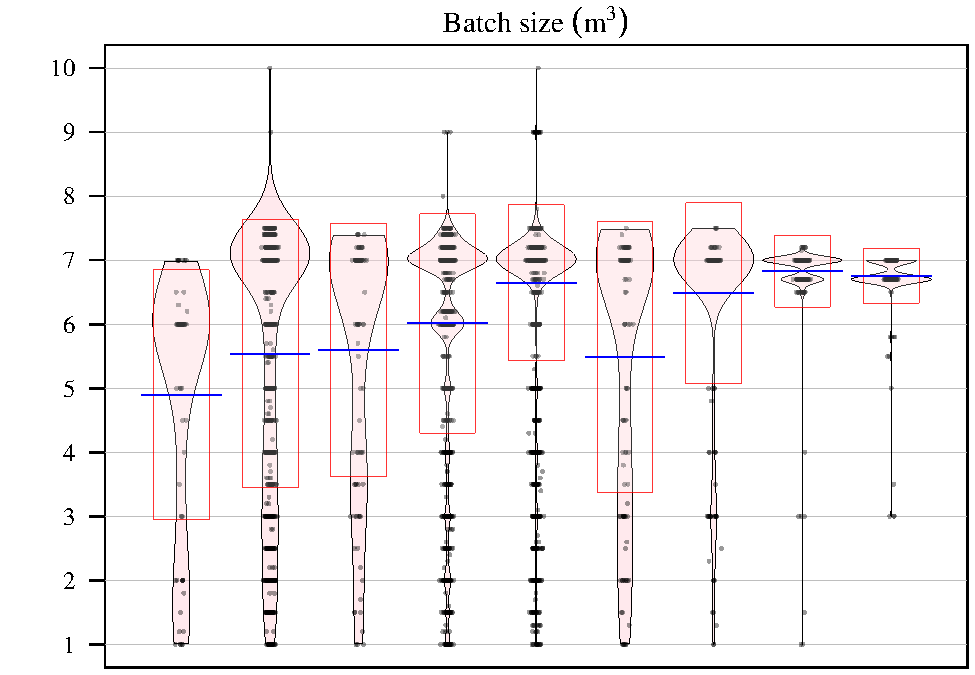
\includegraphics{sl-inf-cairs-2301_files/figure-latex/dataInsights-1} \end{center}

\begin{Shaded}
\begin{Highlighting}[]
\CommentTok{\# Cement}
\FunctionTok{CustPplot}\NormalTok{(}\AttributeTok{formula =}\NormalTok{ Cement}\SpecialCharTok{\textasciitilde{}}\NormalTok{Slump\_class, }\AttributeTok{main =} \FunctionTok{expression}\NormalTok{(Cement}\SpecialCharTok{\textasciitilde{}}\NormalTok{(kg)))}
\end{Highlighting}
\end{Shaded}

\begin{center}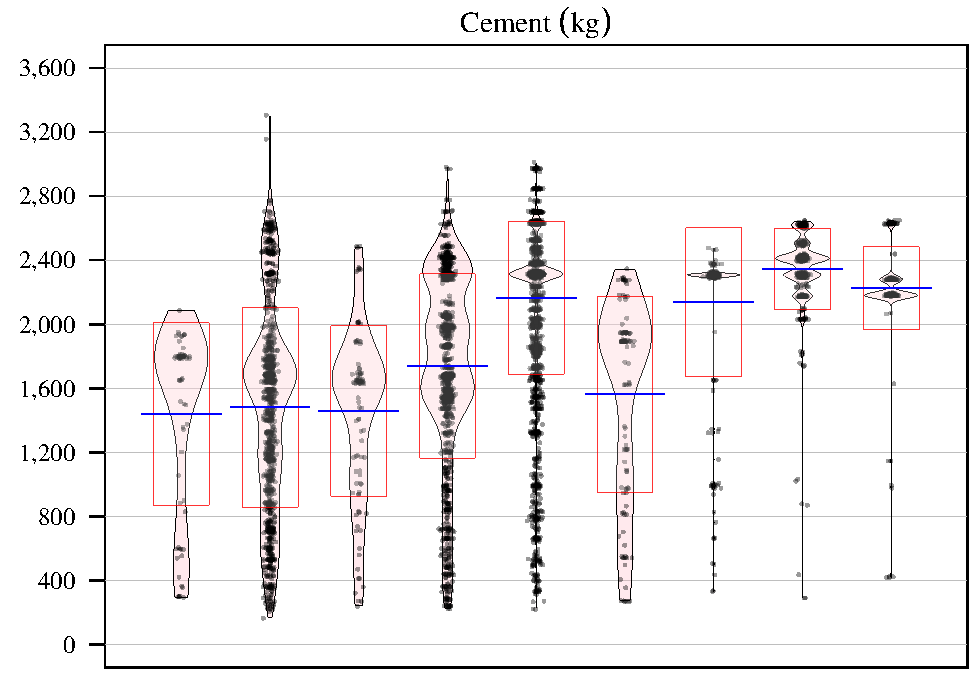
\includegraphics{sl-inf-cairs-2301_files/figure-latex/dataInsights-2} \end{center}

\begin{Shaded}
\begin{Highlighting}[]
\CommentTok{\# Water}
\FunctionTok{CustPplot}\NormalTok{(}\AttributeTok{formula =}\NormalTok{ Water}\SpecialCharTok{\textasciitilde{}}\NormalTok{Slump\_class, }\AttributeTok{main =} \FunctionTok{expression}\NormalTok{(Water}\SpecialCharTok{\textasciitilde{}}\NormalTok{(kg)))}
\end{Highlighting}
\end{Shaded}

\begin{center}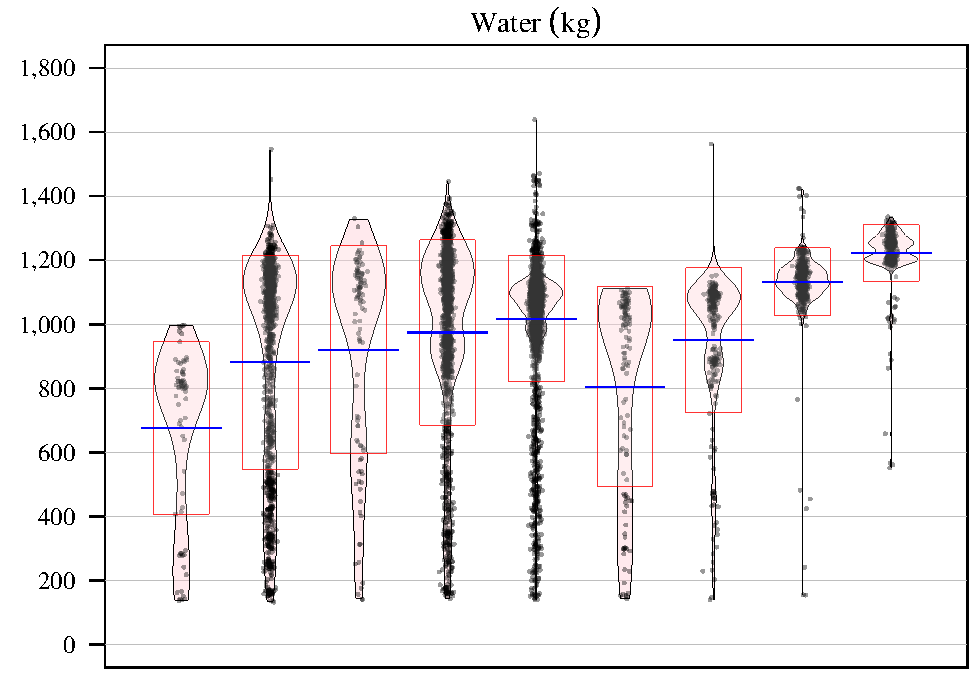
\includegraphics{sl-inf-cairs-2301_files/figure-latex/dataInsights-3} \end{center}

\begin{Shaded}
\begin{Highlighting}[]
\CommentTok{\# Fine aggregated}
\FunctionTok{CustPplot}\NormalTok{(}\AttributeTok{formula =}\NormalTok{ FAG}\SpecialCharTok{\textasciitilde{}}\NormalTok{Slump\_class, }\AttributeTok{main =} \FunctionTok{expression}\NormalTok{(Fine}\SpecialCharTok{\textasciitilde{}}\NormalTok{aggregate}\SpecialCharTok{\textasciitilde{}}\NormalTok{(kg)))}
\end{Highlighting}
\end{Shaded}

\begin{center}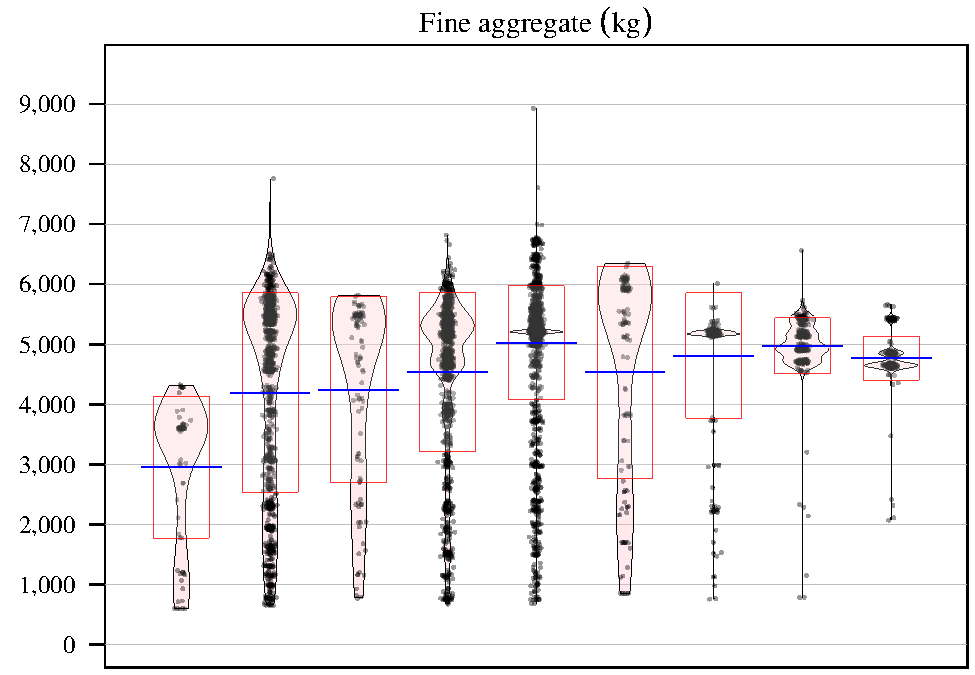
\includegraphics{sl-inf-cairs-2301_files/figure-latex/dataInsights-4} \end{center}

\begin{Shaded}
\begin{Highlighting}[]
\CommentTok{\# Coarse aggregate (10mm)}
\FunctionTok{CustPplot}\NormalTok{(}\AttributeTok{formula =}\NormalTok{ CAG\_10mm}\SpecialCharTok{\textasciitilde{}}\NormalTok{Slump\_class,}
          \AttributeTok{main =} \FunctionTok{expression}\NormalTok{(Coarse}\SpecialCharTok{\textasciitilde{}}\NormalTok{aggregate}\SpecialCharTok{{-}}\FunctionTok{paste}\NormalTok{(}\StringTok{"10mm"}\NormalTok{)))}
\end{Highlighting}
\end{Shaded}

\begin{center}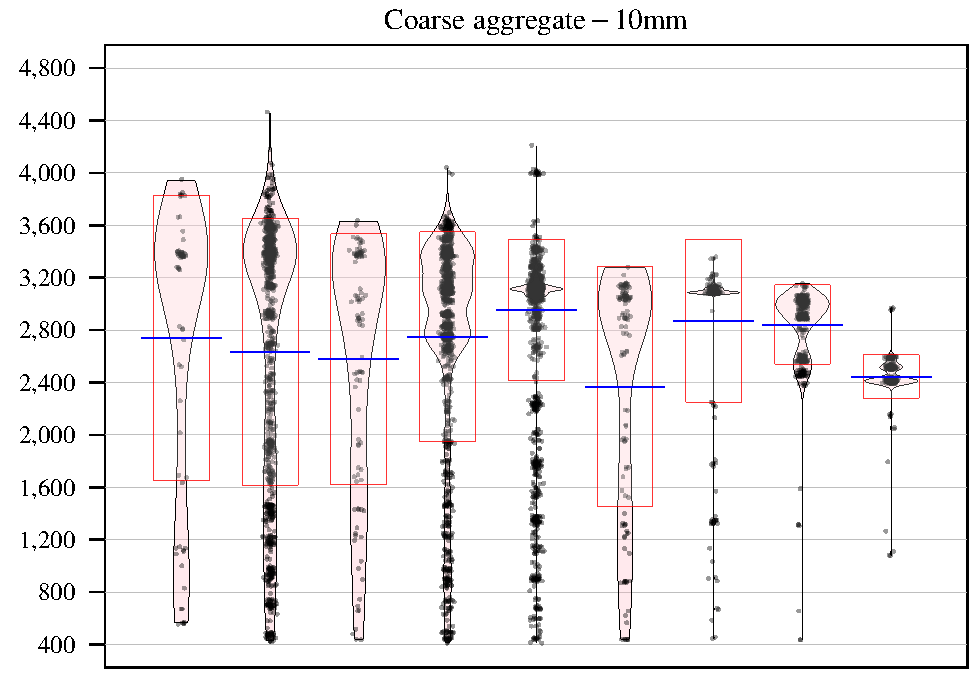
\includegraphics{sl-inf-cairs-2301_files/figure-latex/dataInsights-5} \end{center}

\begin{Shaded}
\begin{Highlighting}[]
\CommentTok{\# Coarse aggregate (20mm)}
\FunctionTok{CustPplot}\NormalTok{(}\AttributeTok{formula =}\NormalTok{ CAG\_20mm}\SpecialCharTok{\textasciitilde{}}\NormalTok{Slump\_class,}
          \AttributeTok{main =} \FunctionTok{expression}\NormalTok{(Coarse}\SpecialCharTok{\textasciitilde{}}\NormalTok{aggregate}\SpecialCharTok{{-}}\FunctionTok{paste}\NormalTok{(}\StringTok{"20mm"}\NormalTok{)}\SpecialCharTok{\textasciitilde{}}\NormalTok{(kg)))}
\end{Highlighting}
\end{Shaded}

\begin{center}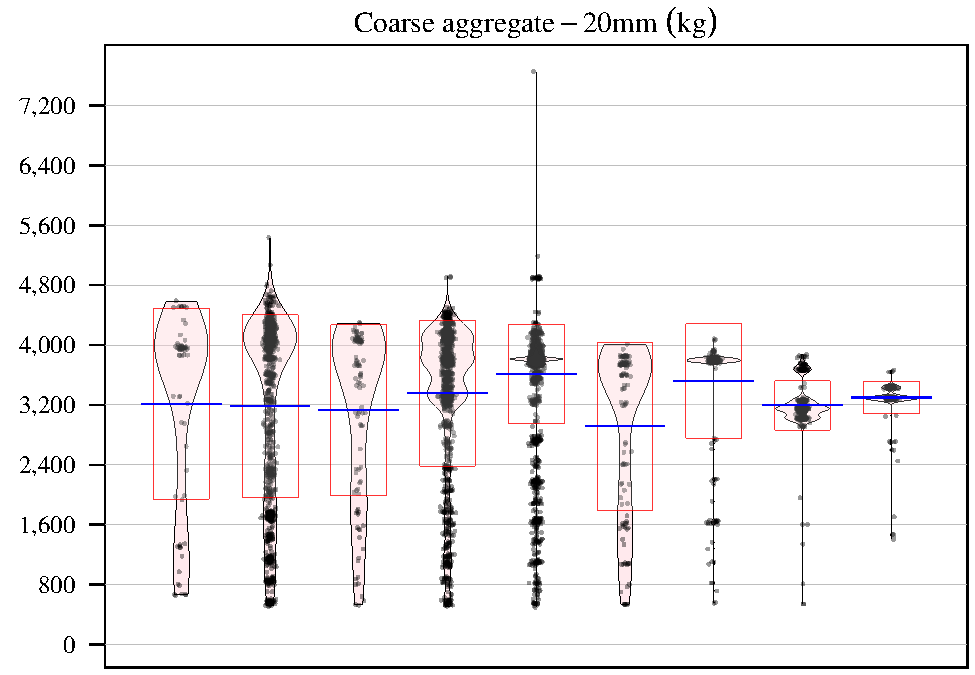
\includegraphics{sl-inf-cairs-2301_files/figure-latex/dataInsights-6} \end{center}

\begin{Shaded}
\begin{Highlighting}[]
\CommentTok{\# Fly ash}
\FunctionTok{CustPplot}\NormalTok{(}\AttributeTok{formula =}\NormalTok{PFA }\SpecialCharTok{\textasciitilde{}}\NormalTok{Slump\_class, }\AttributeTok{main =} \FunctionTok{expression}\NormalTok{(Fly}\SpecialCharTok{\textasciitilde{}}\NormalTok{ash}\SpecialCharTok{\textasciitilde{}}\NormalTok{(kg)))}
\end{Highlighting}
\end{Shaded}

\begin{center}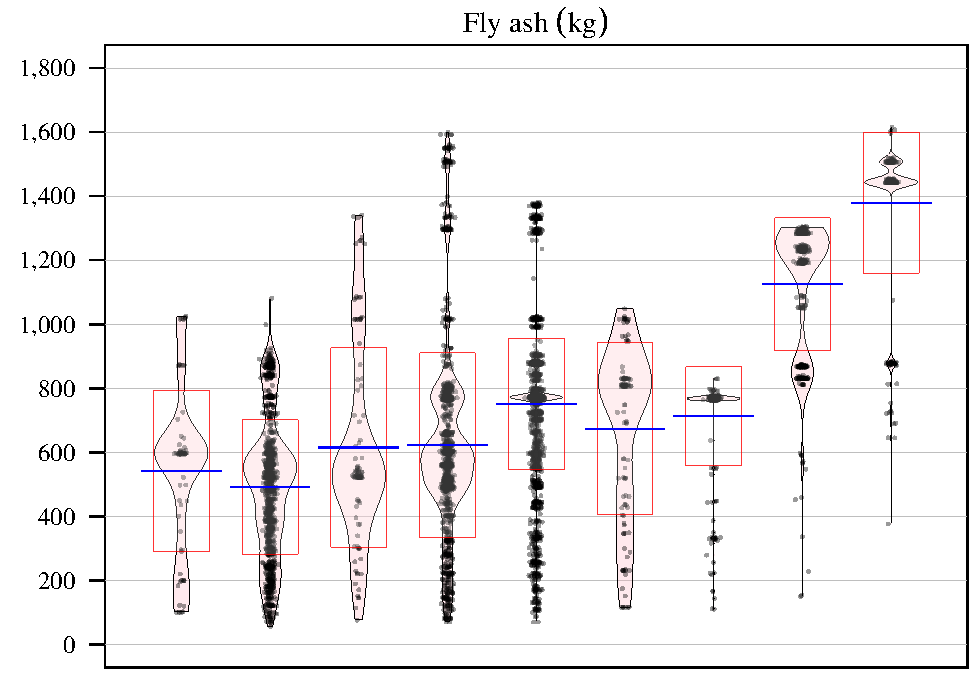
\includegraphics{sl-inf-cairs-2301_files/figure-latex/dataInsights-7} \end{center}

\begin{Shaded}
\begin{Highlighting}[]
\CommentTok{\# Water reducer}
\FunctionTok{CustPplot}\NormalTok{(}\AttributeTok{formula =}\NormalTok{ WRA\_KFDN100}\SpecialCharTok{\textasciitilde{}}\NormalTok{Slump\_class,}
          \AttributeTok{main =} \FunctionTok{expression}\NormalTok{(Water}\SpecialCharTok{\textasciitilde{}}\NormalTok{reducer}\SpecialCharTok{\textasciitilde{}}\NormalTok{(g)))}
\end{Highlighting}
\end{Shaded}

\begin{center}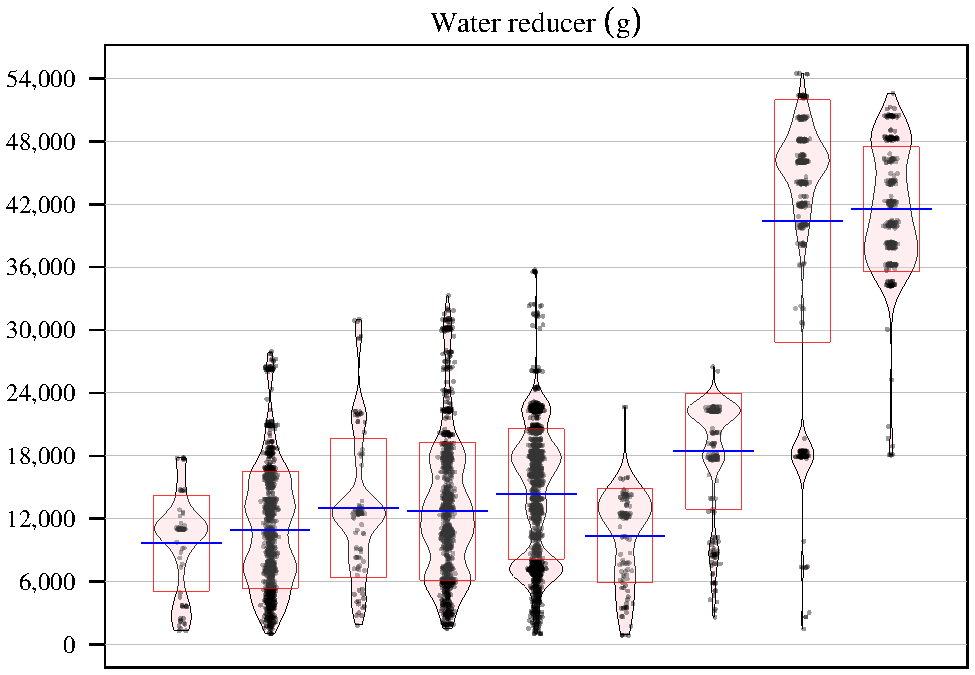
\includegraphics{sl-inf-cairs-2301_files/figure-latex/dataInsights-8} \end{center}

\begin{Shaded}
\begin{Highlighting}[]
\FunctionTok{par}\NormalTok{(}\AttributeTok{family =} \StringTok{"serif"}\NormalTok{, }\AttributeTok{font=}\DecValTok{1}\NormalTok{, }\AttributeTok{mai=}\FunctionTok{c}\NormalTok{(.}\DecValTok{4}\NormalTok{,.}\DecValTok{7}\NormalTok{,.}\DecValTok{3}\NormalTok{,}\FloatTok{0.05}\NormalTok{))}
\CommentTok{\# Superplastisizer1}
\FunctionTok{CustPplot}\NormalTok{(}\AttributeTok{formula =}\NormalTok{ SP1\_KFDNSP8G}\SpecialCharTok{\textasciitilde{}}\NormalTok{Slump\_class, }\AttributeTok{xaxt =} \ConstantTok{NULL}\NormalTok{,}
          \AttributeTok{main =} \FunctionTok{expression}\NormalTok{(Superplasticizer}\SpecialCharTok{{-}}\FunctionTok{paste}\NormalTok{(}\StringTok{"type1"}\NormalTok{)}\SpecialCharTok{\textasciitilde{}}\NormalTok{(g)))}
\end{Highlighting}
\end{Shaded}

\begin{center}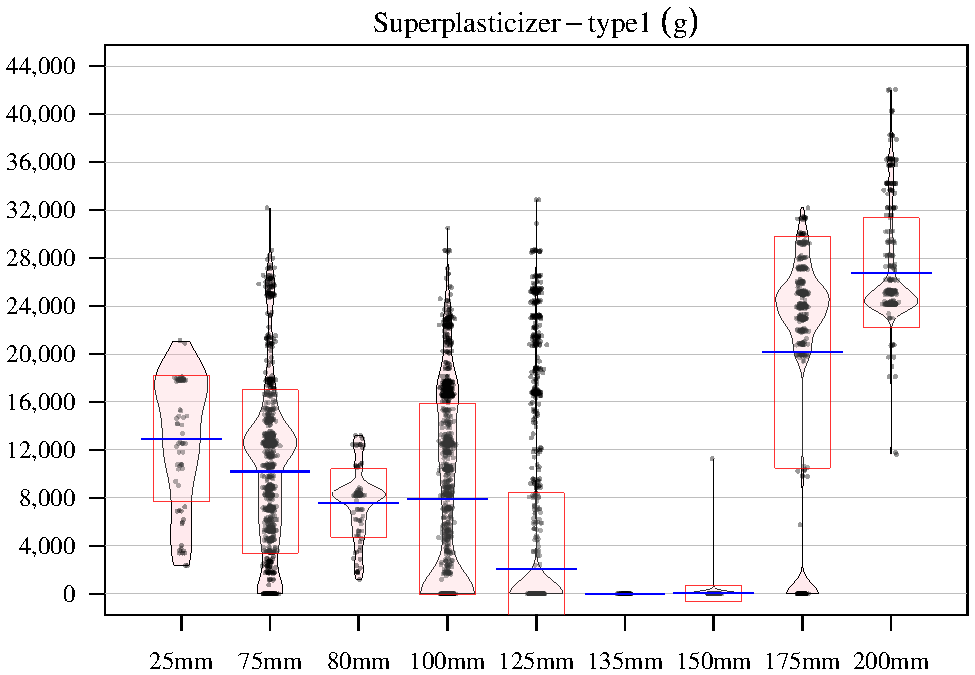
\includegraphics{sl-inf-cairs-2301_files/figure-latex/dataInsights-9} \end{center}

\begin{Shaded}
\begin{Highlighting}[]
\CommentTok{\# Superplastisizer2}
\FunctionTok{CustPplot}\NormalTok{(}\AttributeTok{formula =}\NormalTok{ SP2\_R1002}\SpecialCharTok{\textasciitilde{}}\NormalTok{Slump\_class, }\AttributeTok{xaxt =} \ConstantTok{NULL}\NormalTok{,}
          \AttributeTok{main =} \FunctionTok{expression}\NormalTok{(Superplasticizer}\SpecialCharTok{{-}}\FunctionTok{paste}\NormalTok{(}\StringTok{"type2"}\NormalTok{)}\SpecialCharTok{\textasciitilde{}}\NormalTok{(g)))}
\end{Highlighting}
\end{Shaded}

\begin{center}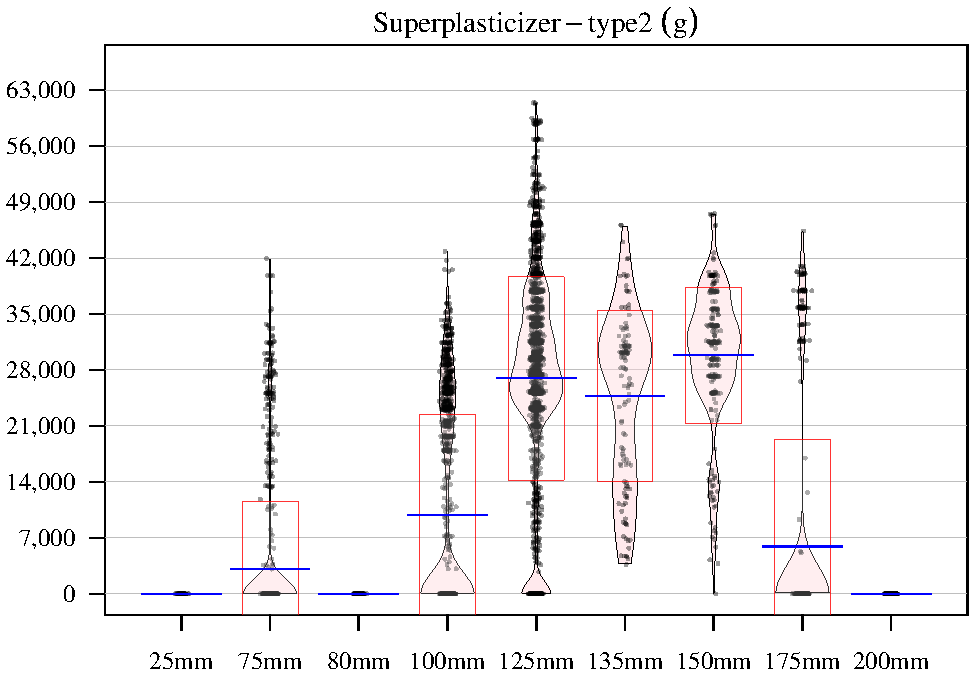
\includegraphics{sl-inf-cairs-2301_files/figure-latex/dataInsights-10} \end{center}

\hypertarget{data-partitioning}{%
\section{Data partitioning}\label{data-partitioning}}

\begin{Shaded}
\begin{Highlighting}[]
\FunctionTok{set.seed}\NormalTok{(}\DecValTok{1226}\NormalTok{) }\CommentTok{\# Setting the seeds to have consistency}
\CommentTok{\# Making index for training data set based on slump class}
\NormalTok{df\_index }\OtherTok{\textless{}{-}} \FunctionTok{createDataPartition}\NormalTok{(df}\SpecialCharTok{$}\NormalTok{Slump\_class, }\AttributeTok{p =} \FloatTok{0.8}\NormalTok{, }\AttributeTok{list=}\ConstantTok{FALSE}\NormalTok{)}
\NormalTok{df\_train }\OtherTok{\textless{}{-}}\NormalTok{ df[df\_index,] ; df\_test }\OtherTok{\textless{}{-}}\NormalTok{ df[}\SpecialCharTok{{-}}\NormalTok{df\_index,]}
\end{Highlighting}
\end{Shaded}

\hypertarget{ml-model-training-and-optimization}{%
\section{ML model training and
optimization}\label{ml-model-training-and-optimization}}

\begin{Shaded}
\begin{Highlighting}[]
\CommentTok{\# Setting the seeds to have consistency}
\FunctionTok{set.seed}\NormalTok{(}\DecValTok{1226}\NormalTok{); seeds }\OtherTok{\textless{}{-}} \FunctionTok{vector}\NormalTok{(}\AttributeTok{mode =} \StringTok{"list"}\NormalTok{, }\AttributeTok{length =} \DecValTok{51}\NormalTok{)}
\ControlFlowTok{for}\NormalTok{ (i }\ControlFlowTok{in} \DecValTok{1}\SpecialCharTok{:}\DecValTok{50}\NormalTok{) seeds[[i]] }\OtherTok{\textless{}{-}} \FunctionTok{sample.int}\NormalTok{(}\DecValTok{1000}\NormalTok{, }\DecValTok{243}\NormalTok{)}
\FunctionTok{set.seed}\NormalTok{(}\DecValTok{1226}\NormalTok{); seeds[[}\DecValTok{51}\NormalTok{]] }\OtherTok{\textless{}{-}} \FunctionTok{sample.int}\NormalTok{(}\DecValTok{1000}\NormalTok{, }\DecValTok{1}\NormalTok{)}
\CommentTok{\# Setting arugments of training}
\NormalTok{train\_Control}\OtherTok{\textless{}{-}}\FunctionTok{trainControl}\NormalTok{(}\StringTok{"repeatedcv"}\NormalTok{, }\AttributeTok{repeats=}\DecValTok{10}\NormalTok{, }\AttributeTok{num=}\DecValTok{5}\NormalTok{, }\AttributeTok{returnData=}\ConstantTok{TRUE}\NormalTok{,}
                            \AttributeTok{classProbs =} \ConstantTok{TRUE}\NormalTok{,  }\AttributeTok{savePredictions =} \StringTok{"all"}\NormalTok{,}
                            \AttributeTok{summaryFunction=}\NormalTok{multiClassSummary,}
                            \AttributeTok{returnResamp=}\StringTok{"all"}\NormalTok{, }\AttributeTok{seeds =}\NormalTok{ seeds)}
\CommentTok{\# Setting the metric for optimization}
\NormalTok{metric }\OtherTok{\textless{}{-}} \StringTok{"logLoss"}
\CommentTok{\# Setting inputs and outputs}
\NormalTok{Form }\OtherTok{\textless{}{-}} \FunctionTok{formula}\NormalTok{(}\StringTok{\textasciigrave{}}\AttributeTok{Slump\_class}\StringTok{\textasciigrave{}}\SpecialCharTok{\textasciitilde{}}\NormalTok{ Batch\_size}\SpecialCharTok{+}\NormalTok{ Cement}\SpecialCharTok{+}\NormalTok{ Water}\SpecialCharTok{+}\NormalTok{ PFA}\SpecialCharTok{+}\NormalTok{ FAG}\SpecialCharTok{+}\NormalTok{ CAG\_10mm}\SpecialCharTok{+}
\NormalTok{                  CAG\_20mm}\SpecialCharTok{+}\NormalTok{ WRA\_KFDN100}\SpecialCharTok{+}\NormalTok{ SP1\_KFDNSP8G}\SpecialCharTok{+}\NormalTok{ SP2\_R1002)}
\CommentTok{\# Setting preprocess method}
\NormalTok{pre\_process }\OtherTok{\textless{}{-}} \FunctionTok{c}\NormalTok{(}\StringTok{"center"}\NormalTok{, }\StringTok{"scale"}\NormalTok{)}
\CommentTok{\# Regularized logistic regression}
\FunctionTok{set.seed}\NormalTok{(}\DecValTok{1226}\NormalTok{)}
\NormalTok{fit\_01regLogistic }\OtherTok{\textless{}{-}} \FunctionTok{train}\NormalTok{(}\AttributeTok{form=}\NormalTok{Form, }\AttributeTok{data=}\NormalTok{df\_train, }\AttributeTok{metric=}\NormalTok{metric,}
                           \AttributeTok{trControl=}\NormalTok{train\_Control, }\AttributeTok{preProcess=}\NormalTok{pre\_process,}
                           \AttributeTok{method=}\StringTok{"regLogistic"}\NormalTok{)}
\CommentTok{\# Generalized linear model}
\FunctionTok{set.seed}\NormalTok{(}\DecValTok{1226}\NormalTok{)}
\NormalTok{fit\_02glmnet }\OtherTok{\textless{}{-}} \FunctionTok{train}\NormalTok{(}\AttributeTok{form=}\NormalTok{Form, }\AttributeTok{data=}\NormalTok{df\_train, }\AttributeTok{metric=}\NormalTok{metric,}
                      \AttributeTok{trControl=}\NormalTok{train\_Control, }\AttributeTok{preProcess=}\NormalTok{pre\_process,}
                      \AttributeTok{method=}\StringTok{"glmnet"}\NormalTok{)}

\CommentTok{\# Linear discriminant analysis: "lda"}
\FunctionTok{set.seed}\NormalTok{(}\DecValTok{1226}\NormalTok{)}
\NormalTok{fit\_03lda }\OtherTok{\textless{}{-}} \FunctionTok{train}\NormalTok{(}\AttributeTok{form=}\NormalTok{Form, }\AttributeTok{data=}\NormalTok{df\_train, }\AttributeTok{metric=}\NormalTok{metric,}
                   \AttributeTok{trControl=}\NormalTok{train\_Control, }\AttributeTok{preProcess=}\NormalTok{pre\_process,}
                   \AttributeTok{method=}\StringTok{"lda"}\NormalTok{)}
\CommentTok{\# Shrinkage discriminant analysis: "sda"}
\FunctionTok{set.seed}\NormalTok{(}\DecValTok{1226}\NormalTok{)}
\NormalTok{fit\_04sda }\OtherTok{\textless{}{-}} \FunctionTok{train}\NormalTok{(}\AttributeTok{form=}\NormalTok{Form,}\AttributeTok{data=}\NormalTok{df\_train, }\AttributeTok{metric=}\NormalTok{metric,}
                   \AttributeTok{trControl=}\NormalTok{train\_Control, }\AttributeTok{preProcess=}\NormalTok{pre\_process,}
                   \AttributeTok{method=}\StringTok{"sda"}\NormalTok{, }\AttributeTok{verbose=}\NormalTok{F)}
\CommentTok{\# Multi layer perceptron: "mlp"}
\FunctionTok{set.seed}\NormalTok{(}\DecValTok{1226}\NormalTok{)}
\NormalTok{fit\_05mlp }\OtherTok{\textless{}{-}} \FunctionTok{train}\NormalTok{(}\AttributeTok{form=}\NormalTok{Form,}\AttributeTok{data=}\NormalTok{df\_train, }\AttributeTok{metric=}\NormalTok{metric,}
                   \AttributeTok{trControl=}\NormalTok{train\_Control, }\AttributeTok{preProcess=}\NormalTok{pre\_process,}
                   \AttributeTok{method=}\StringTok{"mlp"}\NormalTok{)}
\CommentTok{\# Multi layer perceptron with weighted decay parameters: "mlpWeightDecay"}
\FunctionTok{set.seed}\NormalTok{(}\DecValTok{1226}\NormalTok{)}
\NormalTok{fit\_06mlpWD }\OtherTok{\textless{}{-}} \FunctionTok{train}\NormalTok{(}\AttributeTok{form=}\NormalTok{Form,}\AttributeTok{data=}\NormalTok{df\_train, }\AttributeTok{metric=}\NormalTok{metric,}
                     \AttributeTok{trControl=}\NormalTok{train\_Control, }\AttributeTok{preProcess=}\NormalTok{pre\_process,}
                     \AttributeTok{method=}\StringTok{"mlpWeightDecay"}\NormalTok{)}

\CommentTok{\# Multi layer perceptron network with dropout: "mlpKerasDropout"}
\FunctionTok{set.seed}\NormalTok{(}\DecValTok{1226}\NormalTok{)}
\NormalTok{fit\_07mlpKerasDropout }\OtherTok{\textless{}{-}} \FunctionTok{train}\NormalTok{(}\AttributeTok{form=}\NormalTok{Form,}\AttributeTok{data=}\NormalTok{df\_train,}\AttributeTok{trControl=}\NormalTok{train\_Control,}
                               \AttributeTok{metric=}\NormalTok{metric,}\AttributeTok{preProcess=}\NormalTok{pre\_process,}
                               \AttributeTok{method=}\StringTok{"mlpKerasDropout"}\NormalTok{,}\AttributeTok{verbose=}\NormalTok{F)}
\CommentTok{\# Support vector machines with linear kernel: "svmLinear"}
\FunctionTok{set.seed}\NormalTok{(}\DecValTok{1226}\NormalTok{)}
\NormalTok{fit\_08svml }\OtherTok{\textless{}{-}} \FunctionTok{train}\NormalTok{(}\AttributeTok{form=}\NormalTok{Form,}\AttributeTok{data=}\NormalTok{df\_train, }\AttributeTok{metric=}\NormalTok{metric,}
                    \AttributeTok{trControl=}\NormalTok{train\_Control, }\AttributeTok{preProcess=}\NormalTok{pre\_process,}
                    \AttributeTok{method=}\StringTok{"svmLinear"}\NormalTok{)}
\DocumentationTok{\#\# Support vector machines with polynomial kernel: "svmPoly"}
\FunctionTok{set.seed}\NormalTok{(}\DecValTok{1226}\NormalTok{)}
\NormalTok{fit\_09svmp }\OtherTok{\textless{}{-}} \FunctionTok{train}\NormalTok{(}\AttributeTok{form=}\NormalTok{Form, }\AttributeTok{data=}\NormalTok{df\_train, }\AttributeTok{metric=}\NormalTok{metric,}
                    \AttributeTok{trControl=}\NormalTok{train\_Control, }\AttributeTok{preProcess=}\NormalTok{pre\_process,}
                    \AttributeTok{method=}\StringTok{"svmPoly"}\NormalTok{)}
\CommentTok{\# Support vector machines with radial basis function kernel: "svmRadial"}
\FunctionTok{set.seed}\NormalTok{(}\DecValTok{1226}\NormalTok{)}
\NormalTok{fit\_10svmr }\OtherTok{\textless{}{-}} \FunctionTok{train}\NormalTok{(}\AttributeTok{form=}\NormalTok{Form, }\AttributeTok{data=}\NormalTok{df\_train, }\AttributeTok{metric=}\NormalTok{metric,}
                    \AttributeTok{trControl=}\NormalTok{train\_Control, }\AttributeTok{preProcess=}\NormalTok{pre\_process,}
                    \AttributeTok{method=}\StringTok{"svmRadial"}\NormalTok{)}
\CommentTok{\# Classification and regression tree: "rpart2"}
\FunctionTok{set.seed}\NormalTok{(}\DecValTok{1226}\NormalTok{)}
\NormalTok{fit\_11cart }\OtherTok{\textless{}{-}} \FunctionTok{train}\NormalTok{(}\AttributeTok{form=}\NormalTok{Form, }\AttributeTok{data=}\NormalTok{df\_train, }\AttributeTok{metric=}\NormalTok{metric,}
                    \AttributeTok{trControl=}\NormalTok{train\_Control, }\AttributeTok{preProcess=}\NormalTok{pre\_process,}
                    \AttributeTok{method=}\StringTok{"rpart2"}\NormalTok{)}
\CommentTok{\# C5.0 decesion trees: "C5.0"}
\FunctionTok{set.seed}\NormalTok{(}\DecValTok{1226}\NormalTok{)}
\NormalTok{fit\_12C5 }\OtherTok{\textless{}{-}} \FunctionTok{train}\NormalTok{(}\AttributeTok{form=}\NormalTok{Form, }\AttributeTok{data=}\NormalTok{df\_train, }\AttributeTok{metric=}\NormalTok{metric,}
                  \AttributeTok{trControl=}\NormalTok{train\_Control, }\AttributeTok{preProcess=}\NormalTok{pre\_process,}
                  \AttributeTok{method=}\StringTok{"C5.0Tree"}\NormalTok{)}
\CommentTok{\# Random forest: "rf"}
\FunctionTok{set.seed}\NormalTok{(}\DecValTok{1226}\NormalTok{)}
\NormalTok{fit\_13rf }\OtherTok{\textless{}{-}} \FunctionTok{train}\NormalTok{(}\AttributeTok{form=}\NormalTok{Form, }\AttributeTok{data=}\NormalTok{df\_train, }\AttributeTok{metric=}\NormalTok{metric,}
                  \AttributeTok{trControl=}\NormalTok{train\_Control, }\AttributeTok{preProcess=}\NormalTok{pre\_process,}
                  \AttributeTok{method=}\StringTok{"rf"}\NormalTok{)}
\CommentTok{\# Extreme gradient boosting: "xgbTree"}
\FunctionTok{set.seed}\NormalTok{(}\DecValTok{1226}\NormalTok{)}
\NormalTok{fit\_14xgb }\OtherTok{\textless{}{-}} \FunctionTok{train}\NormalTok{(}\AttributeTok{form=}\NormalTok{Form, }\AttributeTok{data=}\NormalTok{df\_train, }\AttributeTok{metric=}\NormalTok{metric,}
                   \AttributeTok{trControl=}\NormalTok{train\_Control, }\AttributeTok{preProcess=}\NormalTok{pre\_process,}
                   \AttributeTok{method=}\StringTok{"xgbTree"}\NormalTok{)}
\end{Highlighting}
\end{Shaded}

\hypertarget{training-performance}{%
\subsection{Training performance}\label{training-performance}}

\begin{Shaded}
\begin{Highlighting}[]
\NormalTok{Model\_list }\OtherTok{\textless{}{-}}
          \FunctionTok{list}\NormalTok{ (}\StringTok{"RLR"}\OtherTok{=}\NormalTok{fit\_01regLogistic,}
                \StringTok{"GLM"} \OtherTok{=}\NormalTok{fit\_02glmnet,}
                \StringTok{"LDA"}\OtherTok{=}\NormalTok{fit\_03lda,}
                \StringTok{"SDA"}\OtherTok{=}\NormalTok{fit\_04sda,}
                \StringTok{"SVM{-}L"}\OtherTok{=}\NormalTok{fit\_08svml,}
                \StringTok{"SVM{-}P"}\OtherTok{=}\NormalTok{fit\_09svmp,}
                \StringTok{"SVM{-}R"}\OtherTok{=}\NormalTok{fit\_10svmr,}
                \StringTok{"MLP"}\OtherTok{=}\NormalTok{fit\_05mlp,}
                \StringTok{"MLP{-}WD"}\OtherTok{=}\NormalTok{fit\_06mlpWD,}
                \StringTok{"MLP{-}D"}\OtherTok{=}\NormalTok{fit\_07mlpKerasDropout,}
                \StringTok{"CART"}\OtherTok{=}\NormalTok{fit\_11cart,}
                \StringTok{"C5.0"}\OtherTok{=}\NormalTok{fit\_12C5,}
                \StringTok{"RF"}\OtherTok{=}\NormalTok{fit\_13rf,}
                \StringTok{"XGBoost"}\OtherTok{=}\NormalTok{fit\_14xgb)}
\CommentTok{\# Getting training results}
\NormalTok{resamp\_list }\OtherTok{\textless{}{-}}\NormalTok{ caret}\SpecialCharTok{::}\FunctionTok{resamples}\NormalTok{(}\AttributeTok{x =}\NormalTok{ Model\_list)}
\CommentTok{\# bwplot(resamp\_list, metric=c("Accuracy","logLoss","Kappa"),}
\CommentTok{\#        layout = c(1,3))}
\CommentTok{\# bwplot(resamp\_list, metric=c("logLoss"))}
\CommentTok{\# bwplot(resamp\_list, metric=c("Kappa"))}
\NormalTok{df\_resamp\_results}\OtherTok{\textless{}{-}}\NormalTok{resamp\_list}\SpecialCharTok{$}\NormalTok{values}
\NormalTok{df\_resamp\_results}\OtherTok{\textless{}{-}}\NormalTok{df\_resamp\_results}\SpecialCharTok{\%\textgreater{}\%}
  \FunctionTok{select}\NormalTok{(.,}\FunctionTok{contains}\NormalTok{(}\AttributeTok{match =}\FunctionTok{c}\NormalTok{(}\StringTok{"\textasciitilde{}Accuracy"}\NormalTok{,}\StringTok{"\textasciitilde{}Kappa"}\NormalTok{,}\StringTok{"\textasciitilde{}logLoss"}\NormalTok{) ))}
\NormalTok{dfmelt}\OtherTok{\textless{}{-}}\FunctionTok{pivot\_longer}\NormalTok{(}\AttributeTok{data =}\NormalTok{ df\_resamp\_results,}\AttributeTok{cols =} \DecValTok{1}\SpecialCharTok{:}\DecValTok{42}\NormalTok{,}
                     \AttributeTok{names\_to =} \StringTok{"Model"}\NormalTok{,}
                     \AttributeTok{values\_to =}\StringTok{"Value"}\NormalTok{)}


\NormalTok{dfmelt[}\FunctionTok{grepl}\NormalTok{(}\AttributeTok{x =}\NormalTok{dfmelt}\SpecialCharTok{$}\NormalTok{Model,}\AttributeTok{pattern =} \StringTok{"\textasciitilde{}Accuracy"}\NormalTok{ ),}\StringTok{"Metric"}\NormalTok{]}\OtherTok{\textless{}{-}}\StringTok{"Accuracy"}
\NormalTok{dfmelt[}\FunctionTok{grepl}\NormalTok{(}\AttributeTok{x =}\NormalTok{dfmelt}\SpecialCharTok{$}\NormalTok{Model,}\AttributeTok{pattern =} \StringTok{"\textasciitilde{}Kappa"}\NormalTok{),}\StringTok{"Metric"}\NormalTok{]}\OtherTok{\textless{}{-}}\StringTok{"Kappa"}
\NormalTok{dfmelt[}\FunctionTok{grepl}\NormalTok{(}\AttributeTok{x =}\NormalTok{dfmelt}\SpecialCharTok{$}\NormalTok{Model,}\AttributeTok{pattern =} \StringTok{"\textasciitilde{}logLoss"}\NormalTok{),}\StringTok{"Metric"}\NormalTok{]}\OtherTok{\textless{}{-}}\StringTok{"logLoss"}
\NormalTok{dfmelt}\SpecialCharTok{$}\NormalTok{Model}\OtherTok{\textless{}{-}}\FunctionTok{gsub}\NormalTok{(}\AttributeTok{x=}\NormalTok{dfmelt}\SpecialCharTok{$}\NormalTok{Model,}\AttributeTok{pattern =} \StringTok{"\textasciitilde{}Accuracy"}\NormalTok{,}\AttributeTok{replacement =} \StringTok{""}\NormalTok{)}
\NormalTok{dfmelt}\SpecialCharTok{$}\NormalTok{Model}\OtherTok{\textless{}{-}}\FunctionTok{gsub}\NormalTok{(}\AttributeTok{x=}\NormalTok{dfmelt}\SpecialCharTok{$}\NormalTok{Model,}\AttributeTok{pattern =} \StringTok{"\textasciitilde{}Kappa"}\NormalTok{,}\AttributeTok{replacement =} \StringTok{""}\NormalTok{)}
\NormalTok{dfmelt}\SpecialCharTok{$}\NormalTok{Model}\OtherTok{\textless{}{-}}\FunctionTok{gsub}\NormalTok{(}\AttributeTok{x=}\NormalTok{dfmelt}\SpecialCharTok{$}\NormalTok{Model,}\AttributeTok{pattern =} \StringTok{"\textasciitilde{}logLoss"}\NormalTok{,}\AttributeTok{replacement =} \StringTok{""}\NormalTok{)}
\NormalTok{dfmelt}\SpecialCharTok{$}\NormalTok{Model}\OtherTok{\textless{}{-}}\FunctionTok{factor}\NormalTok{(dfmelt}\SpecialCharTok{$}\NormalTok{Model,}
                     \AttributeTok{levels =}\NormalTok{ dfmelt}\SpecialCharTok{$}\NormalTok{Model}\SpecialCharTok{\%\textgreater{}\%}\FunctionTok{unique}\NormalTok{())}
\NormalTok{df\_logLoss\_summary}\OtherTok{\textless{}{-}}\NormalTok{dfmelt}\SpecialCharTok{\%\textgreater{}\%}
            \FunctionTok{filter}\NormalTok{(.,Metric}\SpecialCharTok{==}\StringTok{"logLoss"}\NormalTok{)}\SpecialCharTok{\%\textgreater{}\%}
            \FunctionTok{group\_by}\NormalTok{(.,Model)}\SpecialCharTok{\%\textgreater{}\%}
            \FunctionTok{get\_summary\_stats}\NormalTok{(.,}
                              \AttributeTok{show =} \FunctionTok{c}\NormalTok{(}\StringTok{"min"}\NormalTok{,}\StringTok{"max"}\NormalTok{,}\StringTok{"mean"}\NormalTok{,}\StringTok{"median"}\NormalTok{,}\StringTok{"sd"}\NormalTok{,}\StringTok{"se"}\NormalTok{))}


\NormalTok{df\_logLoss\_summary}\SpecialCharTok{\%\textgreater{}\%}\FunctionTok{write.csv}\NormalTok{(}\StringTok{"results/df\_logLoss\_summary.csv"}\NormalTok{)}
\NormalTok{dfmelt}\SpecialCharTok{$}\NormalTok{Model}\OtherTok{\textless{}{-}}\FunctionTok{factor}\NormalTok{(dfmelt}\SpecialCharTok{$}\NormalTok{Model,}
                     \AttributeTok{levels =}\NormalTok{ dfmelt}\SpecialCharTok{$}\NormalTok{Model}\SpecialCharTok{\%\textgreater{}\%}\FunctionTok{unique}\NormalTok{()}\SpecialCharTok{\%\textgreater{}\%}\NormalTok{.[}\DecValTok{14}\SpecialCharTok{:}\DecValTok{1}\NormalTok{])}
\NormalTok{knitr}\SpecialCharTok{::}\FunctionTok{kable}\NormalTok{(df\_logLoss\_summary}\SpecialCharTok{\%\textgreater{}\%}\FunctionTok{select}\NormalTok{(}\SpecialCharTok{!}\FunctionTok{c}\NormalTok{(variable,n))}
\NormalTok{             ,}\AttributeTok{escape =}\NormalTok{ F,}\AttributeTok{digits =} \DecValTok{4}\NormalTok{,}\AttributeTok{format =} \StringTok{"simple"}\NormalTok{)}
\end{Highlighting}
\end{Shaded}

\begin{longtable}[]{@{}lrrrrrr@{}}
\toprule()
Model & min & max & mean & median & sd & se \\
\midrule()
\endhead
RLR & 0.724 & 0.803 & 0.763 & 0.764 & 0.015 & 0.002 \\
GLM & 0.704 & 0.788 & 0.755 & 0.760 & 0.017 & 0.002 \\
LDA & 0.912 & 1.241 & 1.058 & 1.058 & 0.071 & 0.010 \\
SDA & 0.938 & 1.321 & 1.118 & 1.118 & 0.089 & 0.013 \\
SVM-L & 1.165 & 1.242 & 1.199 & 1.196 & 0.016 & 0.002 \\
SVM-P & 1.136 & 1.209 & 1.167 & 1.168 & 0.019 & 0.003 \\
SVM-R & 1.053 & 1.148 & 1.093 & 1.093 & 0.020 & 0.003 \\
MLP & 0.735 & 1.173 & 0.931 & 0.927 & 0.120 & 0.017 \\
MLP-WD & 0.738 & 0.783 & 0.759 & 0.760 & 0.011 & 0.002 \\
MLP-D & 1.916 & 2.602 & 2.248 & 2.243 & 0.127 & 0.018 \\
CART & 0.932 & 1.069 & 0.995 & 0.999 & 0.031 & 0.004 \\
C5.0 & 0.464 & 0.592 & 0.541 & 0.544 & 0.031 & 0.004 \\
RF & 0.284 & 0.457 & 0.360 & 0.349 & 0.045 & 0.006 \\
XGBoost & 0.316 & 0.450 & 0.367 & 0.364 & 0.028 & 0.004 \\
\bottomrule()
\end{longtable}

\begin{Shaded}
\begin{Highlighting}[]
\CommentTok{\# Boxplots}
\NormalTok{bp\_train\_results}\OtherTok{\textless{}{-}}\FunctionTok{ggplot}\NormalTok{(}\AttributeTok{data=}\NormalTok{dfmelt}\SpecialCharTok{\%\textgreater{}\%}\FunctionTok{filter}\NormalTok{(.,Metric}\SpecialCharTok{==}\StringTok{"logLoss"}\NormalTok{),}
                         \FunctionTok{aes}\NormalTok{(}\AttributeTok{x=}\NormalTok{Value, }\AttributeTok{y=}\NormalTok{Model}
                             \CommentTok{\# color=Metric,fill=Metric}
\NormalTok{                             )) }\SpecialCharTok{+}
  \FunctionTok{geom\_boxplot}\NormalTok{(}\AttributeTok{varwidth =} \ConstantTok{TRUE}\NormalTok{,}\AttributeTok{color=}\StringTok{"blue"}\NormalTok{,}
               \AttributeTok{outlier.size =} \DecValTok{0}\NormalTok{,}
               \AttributeTok{outlier.colour =} \ConstantTok{NA}\NormalTok{)}\SpecialCharTok{+}
  \CommentTok{\# facet\_wrap(facets = "Metric",scales="free\_x",nrow = 3)+}
  \FunctionTok{theme\_classic}\NormalTok{()}\SpecialCharTok{+}\FunctionTok{labs}\NormalTok{(}\AttributeTok{x=}\StringTok{"logLoss variation"}\NormalTok{,}\AttributeTok{y=}\StringTok{""}\NormalTok{)}\SpecialCharTok{+}
  \FunctionTok{theme}\NormalTok{(}\AttributeTok{axis.text.y =} \FunctionTok{element\_text}\NormalTok{(}\AttributeTok{colour =} \StringTok{"black"}\NormalTok{,}\AttributeTok{size=}\DecValTok{12}\NormalTok{,}
                                   \AttributeTok{margin =}\FunctionTok{margin}\NormalTok{(}\AttributeTok{t =} \DecValTok{5}\NormalTok{, }\AttributeTok{r =} \DecValTok{1}\NormalTok{, }\AttributeTok{b =} \DecValTok{5}\NormalTok{, }\AttributeTok{l =} \DecValTok{1}\NormalTok{,}
                                                  \AttributeTok{unit =} \StringTok{"pt"}\NormalTok{)),}
                \AttributeTok{axis.text =} \FunctionTok{element\_text}\NormalTok{(}\AttributeTok{colour =} \StringTok{"black"}\NormalTok{,}\AttributeTok{size=}\DecValTok{11}\NormalTok{),}
        \AttributeTok{axis.title =} \FunctionTok{element\_text}\NormalTok{(}\AttributeTok{colour =} \StringTok{"black"}\NormalTok{,}\AttributeTok{size=}\DecValTok{12}\NormalTok{),}
        \AttributeTok{legend.title =} \FunctionTok{element\_blank}\NormalTok{(),}
        \AttributeTok{legend.position=}\StringTok{"none"}\NormalTok{,}
        \CommentTok{\# \# strip.text = element\_text("logLoss variation",size = 12),}
        \CommentTok{\# \# strip.background = element\_rect(fill = "White"),}
        \CommentTok{\# \# panel.spacing = unit(1, "lines"),}
        \CommentTok{\# axis.line.x.bottom = element\_line(colour = "black"),}
        \CommentTok{\# \# plot.margin = margin(t = 10, r = 15, b = 10, l = 5, unit = "pt")}
\NormalTok{        )}\SpecialCharTok{+}
  \CommentTok{\# scale\_colour\_manual(values = rainbow(3))+}
  \FunctionTok{scale\_x\_continuous}\NormalTok{(}\AttributeTok{breaks =} \FunctionTok{seq}\NormalTok{(}\FloatTok{0.5}\NormalTok{,}\FloatTok{2.5}\NormalTok{,}\FloatTok{0.5}\NormalTok{))}
\NormalTok{bp\_train\_results}
\end{Highlighting}
\end{Shaded}

\begin{center}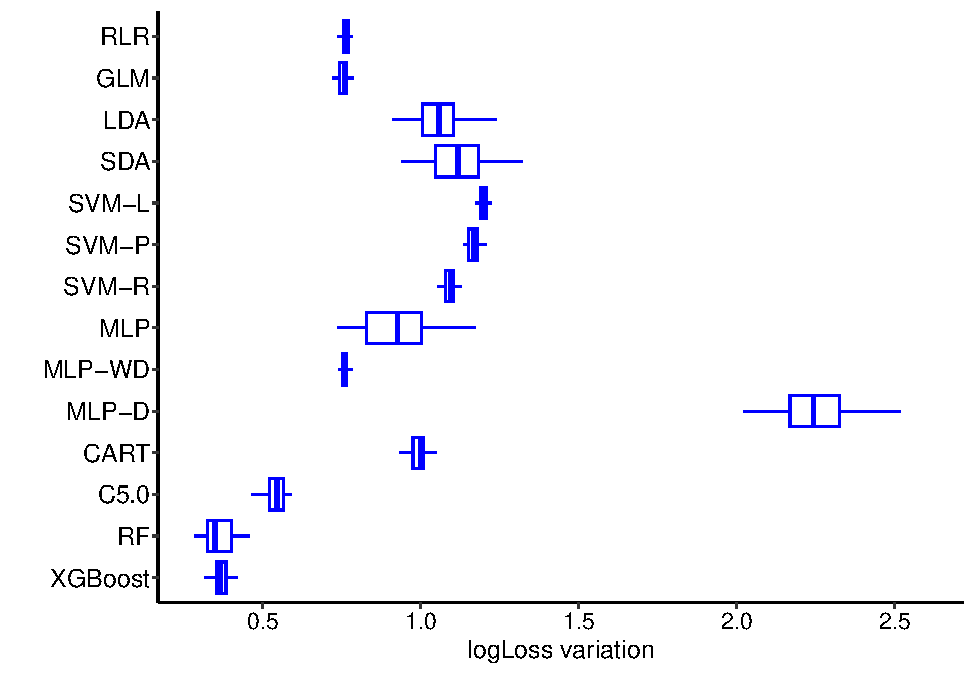
\includegraphics{sl-inf-cairs-2301_files/figure-latex/trainResults-1} \end{center}

\begin{Shaded}
\begin{Highlighting}[]
\CommentTok{\# http://127.0.0.1:20991/graphics/plot\_zoom\_png?width=718\&height=404}
\FunctionTok{ggsave}\NormalTok{(}\AttributeTok{plot =} \FunctionTok{last\_plot}\NormalTok{(),}\AttributeTok{filename =} \StringTok{"results/bp\_train.jpeg"}\NormalTok{,}\AttributeTok{device =} \StringTok{"jpeg"}\NormalTok{,}\AttributeTok{dpi=}\DecValTok{600}\NormalTok{,}
       \AttributeTok{height =} \DecValTok{404}\SpecialCharTok{/}\DecValTok{96}\NormalTok{,}\AttributeTok{width =} \DecValTok{718}\SpecialCharTok{/}\DecValTok{96}\NormalTok{)}
\end{Highlighting}
\end{Shaded}

\begin{quote}
\hypertarget{optimization-hyperparameter-tunning-results}{%
\subsubsection{Optimization (Hyperparameter tunning)
results}\label{optimization-hyperparameter-tunning-results}}
\end{quote}

\begin{Shaded}
\begin{Highlighting}[]
\NormalTok{df\_hp\_rlr}\OtherTok{\textless{}{-}}\NormalTok{fit\_01regLogistic}\SpecialCharTok{$}\NormalTok{results}
\NormalTok{df\_hp\_rlr}\SpecialCharTok{$}\NormalTok{loss}\OtherTok{\textless{}{-}}\FunctionTok{as.factor}\NormalTok{(df\_hp\_rlr}\SpecialCharTok{$}\NormalTok{loss)}
\NormalTok{plt\_rlr}\OtherTok{\textless{}{-}}\FunctionTok{ggplot}\NormalTok{(}\AttributeTok{data=}\NormalTok{df\_hp\_rlr, }\FunctionTok{aes}\NormalTok{(}\AttributeTok{y =}\NormalTok{ logLoss, }\AttributeTok{x =}\NormalTok{ cost, }\AttributeTok{color=}\NormalTok{loss)) }\SpecialCharTok{+}
  \FunctionTok{geom\_point}\NormalTok{() }\SpecialCharTok{+} \FunctionTok{geom\_line}\NormalTok{() }\SpecialCharTok{+} \FunctionTok{theme\_classic}\NormalTok{()}\SpecialCharTok{+}
  \FunctionTok{facet\_wrap}\NormalTok{(. }\SpecialCharTok{\textasciitilde{}}\NormalTok{epsilon, }\AttributeTok{ncol =} \DecValTok{3}\NormalTok{,}\AttributeTok{labeller =}\NormalTok{label\_both)}\SpecialCharTok{+}
  \FunctionTok{labs}\NormalTok{(}\AttributeTok{color=}\StringTok{"loss"}\NormalTok{,}\AttributeTok{x=}\FunctionTok{expression}\NormalTok{(cost),}\AttributeTok{y=}\StringTok{""}\NormalTok{)}\SpecialCharTok{+}
  \FunctionTok{ggtitle}\NormalTok{(}\StringTok{"RLR"}\NormalTok{)}\SpecialCharTok{+}
  \FunctionTok{theme}\NormalTok{(}\AttributeTok{legend.position =} \StringTok{"right"}\NormalTok{,}
        \AttributeTok{axis.title =} \FunctionTok{element\_text}\NormalTok{(}\AttributeTok{face =} \StringTok{"plain"}\NormalTok{,}\AttributeTok{size =} \DecValTok{11}\NormalTok{,}\AttributeTok{color =} \StringTok{"black"}\NormalTok{),}
        \AttributeTok{axis.text =} \FunctionTok{element\_text}\NormalTok{(}\AttributeTok{face =} \StringTok{"plain"}\NormalTok{,}\AttributeTok{size =} \DecValTok{11}\NormalTok{,}\AttributeTok{color =} \StringTok{"black"}\NormalTok{),}
        \AttributeTok{strip.text =} \FunctionTok{element\_text}\NormalTok{(}\AttributeTok{face =} \StringTok{"plain"}\NormalTok{,}\AttributeTok{size =} \DecValTok{11}\NormalTok{),}
        \AttributeTok{legend.title =} \FunctionTok{element\_text}\NormalTok{(}\AttributeTok{face =} \StringTok{"plain"}\NormalTok{,}\AttributeTok{size =} \DecValTok{11}\NormalTok{),}
        \AttributeTok{legend.text =} \FunctionTok{element\_text}\NormalTok{(}\AttributeTok{face =} \StringTok{"plain"}\NormalTok{,}\AttributeTok{size =} \DecValTok{11}\NormalTok{),}
        \AttributeTok{panel.spacing =} \FunctionTok{unit}\NormalTok{(}\DecValTok{1}\NormalTok{, }\StringTok{"lines"}\NormalTok{))}\SpecialCharTok{+}
  \FunctionTok{scale\_x\_continuous}\NormalTok{(}\AttributeTok{breaks =} \FunctionTok{c}\NormalTok{(}\FloatTok{0.5}\NormalTok{,}\FloatTok{1.0}\NormalTok{,}\FloatTok{2.0}\NormalTok{))}\SpecialCharTok{+}
  \FunctionTok{scale\_y\_continuous}\NormalTok{(}\AttributeTok{breaks =} \FunctionTok{round}\NormalTok{(}\FunctionTok{seq}\NormalTok{(}\FloatTok{0.76}\NormalTok{,}\FloatTok{0.872}\NormalTok{,}\AttributeTok{length.out=}\DecValTok{5}\NormalTok{),}\DecValTok{3}\NormalTok{),}
                     \AttributeTok{limits =} \FunctionTok{c}\NormalTok{(}\FloatTok{0.76}\NormalTok{,.}\DecValTok{872}\NormalTok{))}
\NormalTok{plt\_rlr}
\end{Highlighting}
\end{Shaded}

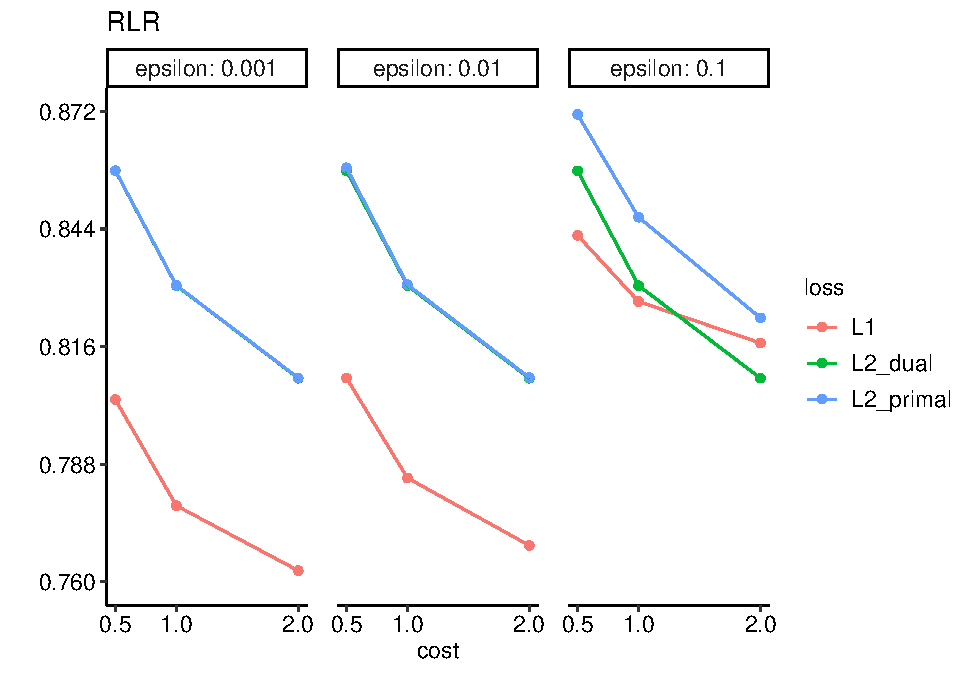
\includegraphics{sl-inf-cairs-2301_files/figure-latex/optResults-1.pdf}

\begin{Shaded}
\begin{Highlighting}[]
\NormalTok{df\_hp\_glm}\OtherTok{\textless{}{-}}\NormalTok{fit\_02glmnet}\SpecialCharTok{$}\NormalTok{results}
\NormalTok{df\_hp\_glm}\SpecialCharTok{$}\NormalTok{lambda}\OtherTok{\textless{}{-}}\FunctionTok{signif}\NormalTok{(df\_hp\_glm}\SpecialCharTok{$}\NormalTok{lambda,}\DecValTok{1}\NormalTok{)}
\NormalTok{df\_hp\_glm}\SpecialCharTok{$}\NormalTok{lambda}\OtherTok{\textless{}{-}}\FunctionTok{sprintf}\NormalTok{(}\StringTok{"\%.4f"}\NormalTok{,df\_hp\_glm}\SpecialCharTok{$}\NormalTok{lambda)}
\NormalTok{plt\_glm}\OtherTok{\textless{}{-}}\FunctionTok{ggplot}\NormalTok{(}\AttributeTok{data=}\NormalTok{df\_hp\_glm, }\FunctionTok{aes}\NormalTok{(}\AttributeTok{y =}\NormalTok{ logLoss, }\AttributeTok{x =}\NormalTok{ alpha,}\AttributeTok{color=}\NormalTok{lambda)) }\SpecialCharTok{+}
  \FunctionTok{geom\_point}\NormalTok{() }\SpecialCharTok{+} \FunctionTok{geom\_line}\NormalTok{() }\SpecialCharTok{+} \FunctionTok{theme\_classic}\NormalTok{()}\SpecialCharTok{+}
  \CommentTok{\# facet\_wrap(. \textasciitilde{}epsilon, ncol = 3,labeller =label\_both)+}
  \FunctionTok{labs}\NormalTok{(}\AttributeTok{color=}\FunctionTok{expression}\NormalTok{(lambda),}\AttributeTok{x=}\FunctionTok{expression}\NormalTok{(alpha),}\AttributeTok{y=}\StringTok{""}\NormalTok{) }\SpecialCharTok{+}
  \FunctionTok{ggtitle}\NormalTok{(}\StringTok{"GLM"}\NormalTok{)}\SpecialCharTok{+}
  \FunctionTok{theme}\NormalTok{(}\AttributeTok{legend.position =} \StringTok{"right"}\NormalTok{,}
        \AttributeTok{axis.title =} \FunctionTok{element\_text}\NormalTok{(}\AttributeTok{face =} \StringTok{"plain"}\NormalTok{,}\AttributeTok{size =} \DecValTok{11}\NormalTok{,}\AttributeTok{color =} \StringTok{"black"}\NormalTok{),}
        \AttributeTok{axis.text =} \FunctionTok{element\_text}\NormalTok{(}\AttributeTok{face =} \StringTok{"plain"}\NormalTok{,}\AttributeTok{size =} \DecValTok{11}\NormalTok{,}\AttributeTok{color =} \StringTok{"black"}\NormalTok{),}
        \AttributeTok{strip.text =} \FunctionTok{element\_text}\NormalTok{(}\AttributeTok{face =} \StringTok{"plain"}\NormalTok{,}\AttributeTok{size =} \DecValTok{11}\NormalTok{),}
        \AttributeTok{legend.title =} \FunctionTok{element\_text}\NormalTok{(}\AttributeTok{face =} \StringTok{"plain"}\NormalTok{,}\AttributeTok{size =} \DecValTok{11}\NormalTok{),}
        \AttributeTok{legend.text =} \FunctionTok{element\_text}\NormalTok{(}\AttributeTok{face =} \StringTok{"plain"}\NormalTok{,}\AttributeTok{size =} \DecValTok{11}\NormalTok{),}
        \AttributeTok{panel.spacing =} \FunctionTok{unit}\NormalTok{(}\DecValTok{1}\NormalTok{, }\StringTok{"lines"}\NormalTok{))}\SpecialCharTok{+}
  \FunctionTok{scale\_x\_continuous}\NormalTok{(}\AttributeTok{breaks =} \FunctionTok{c}\NormalTok{(}\FloatTok{0.1}\NormalTok{,.}\DecValTok{55}\NormalTok{,}\FloatTok{1.0}\NormalTok{))}\SpecialCharTok{+}
  \FunctionTok{scale\_y\_continuous}\NormalTok{(}\AttributeTok{breaks =} \FunctionTok{round}\NormalTok{(}\FunctionTok{seq}\NormalTok{(}\FloatTok{0.75}\NormalTok{,}\FloatTok{1.25}\NormalTok{,}\AttributeTok{length.out=}\DecValTok{5}\NormalTok{),}\DecValTok{3}\NormalTok{)}
\NormalTok{                     ,}\AttributeTok{limits =} \FunctionTok{c}\NormalTok{(}\FloatTok{0.75}\NormalTok{,}\FloatTok{1.24}\NormalTok{))}
\NormalTok{plt\_glm}
\end{Highlighting}
\end{Shaded}

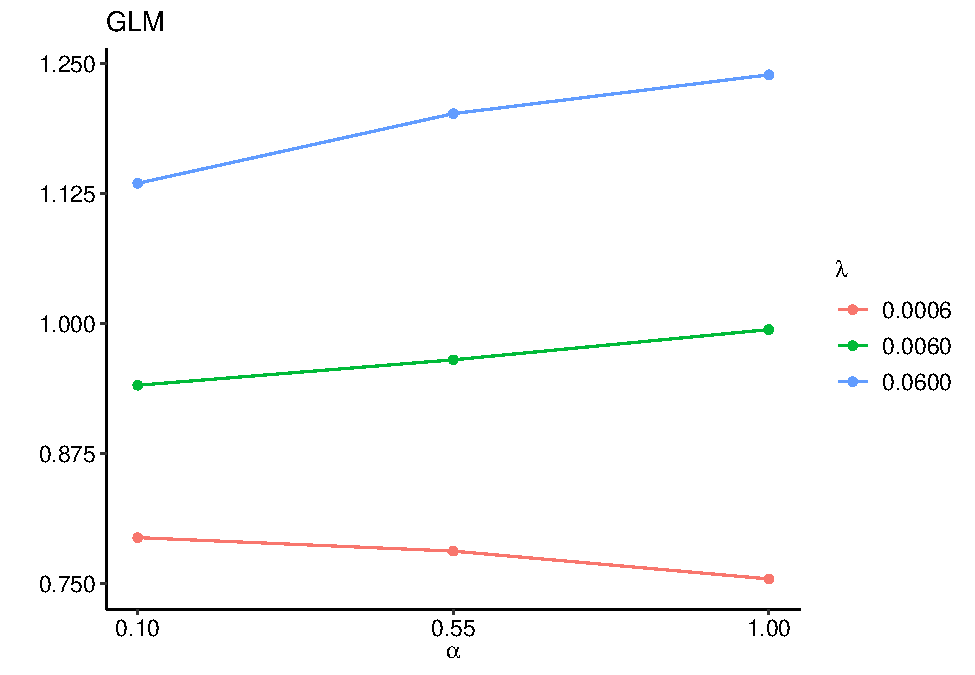
\includegraphics{sl-inf-cairs-2301_files/figure-latex/optResults-2.pdf}

\begin{Shaded}
\begin{Highlighting}[]
\CommentTok{\# df\_hp\_glm\textless{}{-}fit\_02glmnet$results}
\CommentTok{\# df\_hp\_glm$lambda\textless{}{-}signif(df\_hp\_glm$lambda,1)}
\CommentTok{\# df\_hp\_glm$lambda\textless{}{-}as.factor(df\_hp\_glm$lambda)}
\NormalTok{plt\_sda}\OtherTok{\textless{}{-}}\FunctionTok{ggplot}\NormalTok{(}\AttributeTok{data=}\NormalTok{fit\_04sda}\SpecialCharTok{$}\NormalTok{results,}
                \FunctionTok{aes}\NormalTok{(}\AttributeTok{y =}\NormalTok{ logLoss, }\AttributeTok{x =}\NormalTok{ lambda)) }\SpecialCharTok{+}
  \FunctionTok{geom\_point}\NormalTok{() }\SpecialCharTok{+} \FunctionTok{geom\_line}\NormalTok{() }\SpecialCharTok{+} \FunctionTok{theme\_classic}\NormalTok{()}\SpecialCharTok{+}
  \CommentTok{\# facet\_wrap(. \textasciitilde{}epsilon, ncol = 3,labeller =label\_both)+}
  \FunctionTok{labs}\NormalTok{(}\AttributeTok{color=}\StringTok{"loss function"}\NormalTok{,}\AttributeTok{x=}\FunctionTok{expression}\NormalTok{(lambda),}\AttributeTok{y=}\StringTok{""}\NormalTok{) }\SpecialCharTok{+}
  \FunctionTok{ggtitle}\NormalTok{(}\StringTok{"SDA"}\NormalTok{)}\SpecialCharTok{+}
  \FunctionTok{theme}\NormalTok{(}\AttributeTok{legend.position =} \StringTok{"right"}\NormalTok{,}
        \AttributeTok{axis.title =} \FunctionTok{element\_text}\NormalTok{(}\AttributeTok{face =} \StringTok{"plain"}\NormalTok{,}\AttributeTok{size =} \DecValTok{11}\NormalTok{,}\AttributeTok{color =} \StringTok{"black"}\NormalTok{),}
        \AttributeTok{axis.text =} \FunctionTok{element\_text}\NormalTok{(}\AttributeTok{face =} \StringTok{"plain"}\NormalTok{,}\AttributeTok{size =} \DecValTok{11}\NormalTok{,}\AttributeTok{color =} \StringTok{"black"}\NormalTok{),}
        \AttributeTok{strip.text =} \FunctionTok{element\_text}\NormalTok{(}\AttributeTok{face =} \StringTok{"plain"}\NormalTok{,}\AttributeTok{size =} \DecValTok{11}\NormalTok{),}
        \AttributeTok{legend.title =} \FunctionTok{element\_text}\NormalTok{(}\AttributeTok{face =} \StringTok{"plain"}\NormalTok{,}\AttributeTok{size =} \DecValTok{11}\NormalTok{),}
        \AttributeTok{legend.text =} \FunctionTok{element\_text}\NormalTok{(}\AttributeTok{face =} \StringTok{"plain"}\NormalTok{,}\AttributeTok{size =} \DecValTok{11}\NormalTok{),}
        \AttributeTok{panel.spacing =} \FunctionTok{unit}\NormalTok{(}\DecValTok{1}\NormalTok{, }\StringTok{"lines"}\NormalTok{))}\SpecialCharTok{+}
  \FunctionTok{scale\_x\_continuous}\NormalTok{(}\AttributeTok{breaks =} \FunctionTok{c}\NormalTok{(}\DecValTok{0}\NormalTok{,.}\DecValTok{5}\NormalTok{,}\FloatTok{1.0}\NormalTok{))}\SpecialCharTok{+}
  \FunctionTok{scale\_y\_continuous}\NormalTok{(}\AttributeTok{breaks =} \FunctionTok{round}\NormalTok{(}\FunctionTok{seq}\NormalTok{(}\FloatTok{1.111}\NormalTok{,}\FloatTok{2.270}\NormalTok{,}\AttributeTok{length.out=}\DecValTok{5}\NormalTok{),}\DecValTok{3}\NormalTok{),}
                     \AttributeTok{limits =} \FunctionTok{c}\NormalTok{(}\FloatTok{1.111}\NormalTok{,}\FloatTok{2.27}\NormalTok{))}
\NormalTok{plt\_sda}
\end{Highlighting}
\end{Shaded}

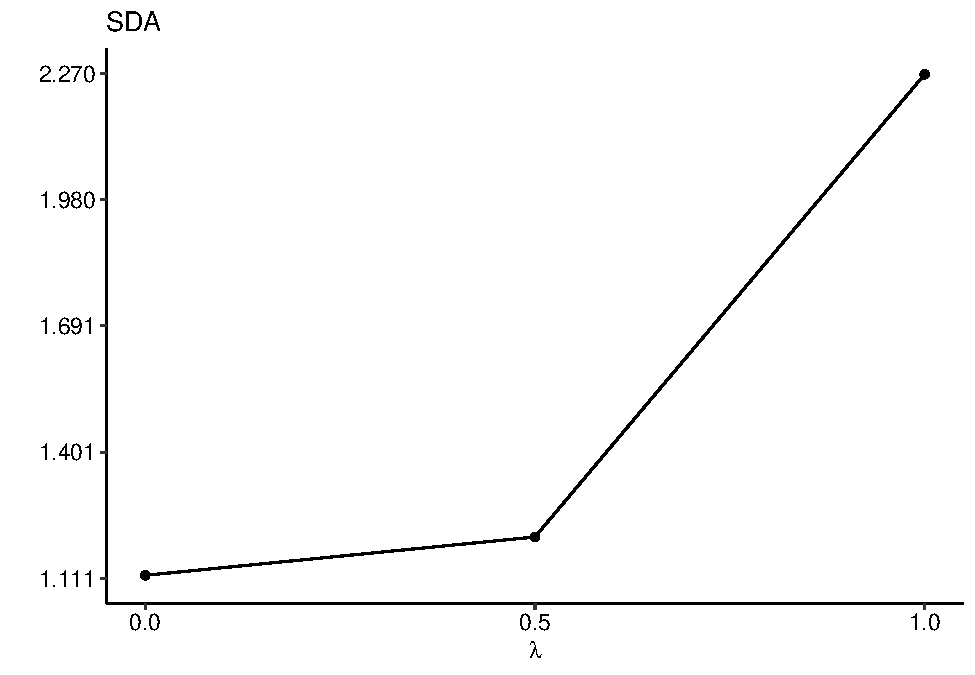
\includegraphics{sl-inf-cairs-2301_files/figure-latex/optResults-3.pdf}

\begin{Shaded}
\begin{Highlighting}[]
\NormalTok{plt\_mlp}\OtherTok{\textless{}{-}}\FunctionTok{ggplot}\NormalTok{(}\AttributeTok{data=}\NormalTok{fit\_05mlp}\SpecialCharTok{$}\NormalTok{results,}
                \FunctionTok{aes}\NormalTok{(}\AttributeTok{y =}\NormalTok{ logLoss, }\AttributeTok{x =}\NormalTok{ size)) }\SpecialCharTok{+}
  \FunctionTok{geom\_point}\NormalTok{() }\SpecialCharTok{+} \FunctionTok{geom\_line}\NormalTok{() }\SpecialCharTok{+} \FunctionTok{theme\_classic}\NormalTok{()}\SpecialCharTok{+}
  \CommentTok{\# facet\_wrap(. \textasciitilde{}epsilon, ncol = 3,labeller =label\_both)+}
  \FunctionTok{labs}\NormalTok{(}\AttributeTok{color=}\StringTok{"loss function"}\NormalTok{,}\AttributeTok{x=}\StringTok{"size"}\NormalTok{,}\AttributeTok{y=}\StringTok{""}\NormalTok{) }\SpecialCharTok{+}
  \FunctionTok{ggtitle}\NormalTok{(}\StringTok{"MLP"}\NormalTok{)}\SpecialCharTok{+}
  \FunctionTok{theme}\NormalTok{(}\AttributeTok{legend.position =} \StringTok{"right"}\NormalTok{,}
        \AttributeTok{axis.title =} \FunctionTok{element\_text}\NormalTok{(}\AttributeTok{face =} \StringTok{"plain"}\NormalTok{,}\AttributeTok{size =} \DecValTok{11}\NormalTok{,}\AttributeTok{color =} \StringTok{"black"}\NormalTok{),}
        \AttributeTok{axis.text =} \FunctionTok{element\_text}\NormalTok{(}\AttributeTok{face =} \StringTok{"plain"}\NormalTok{,}\AttributeTok{size =} \DecValTok{11}\NormalTok{,}\AttributeTok{color =} \StringTok{"black"}\NormalTok{),}
        \AttributeTok{strip.text =} \FunctionTok{element\_text}\NormalTok{(}\AttributeTok{face =} \StringTok{"plain"}\NormalTok{,}\AttributeTok{size =} \DecValTok{11}\NormalTok{),}
        \AttributeTok{legend.title =} \FunctionTok{element\_text}\NormalTok{(}\AttributeTok{face =} \StringTok{"plain"}\NormalTok{,}\AttributeTok{size =} \DecValTok{11}\NormalTok{),}
        \AttributeTok{legend.text =} \FunctionTok{element\_text}\NormalTok{(}\AttributeTok{face =} \StringTok{"plain"}\NormalTok{,}\AttributeTok{size =} \DecValTok{11}\NormalTok{),}
        \AttributeTok{panel.spacing =} \FunctionTok{unit}\NormalTok{(}\DecValTok{1}\NormalTok{, }\StringTok{"lines"}\NormalTok{))}\SpecialCharTok{+}
  \FunctionTok{scale\_x\_continuous}\NormalTok{(}\AttributeTok{breaks =} \FunctionTok{c}\NormalTok{(}\DecValTok{1}\NormalTok{,}\DecValTok{3}\NormalTok{,}\FloatTok{5.0}\NormalTok{))}\SpecialCharTok{+}
  \FunctionTok{scale\_y\_continuous}\NormalTok{(}\AttributeTok{breaks =} \FunctionTok{round}\NormalTok{(}\FunctionTok{seq}\NormalTok{(}\FloatTok{0.93}\NormalTok{,}\FloatTok{1.54}\NormalTok{,}\AttributeTok{length.out=}\DecValTok{5}\NormalTok{),}\DecValTok{3}\NormalTok{)}
\NormalTok{                     ,}\AttributeTok{limits =} \FunctionTok{c}\NormalTok{(}\FloatTok{0.93}\NormalTok{,}\FloatTok{1.54}\NormalTok{))}
\NormalTok{plt\_mlp}
\end{Highlighting}
\end{Shaded}

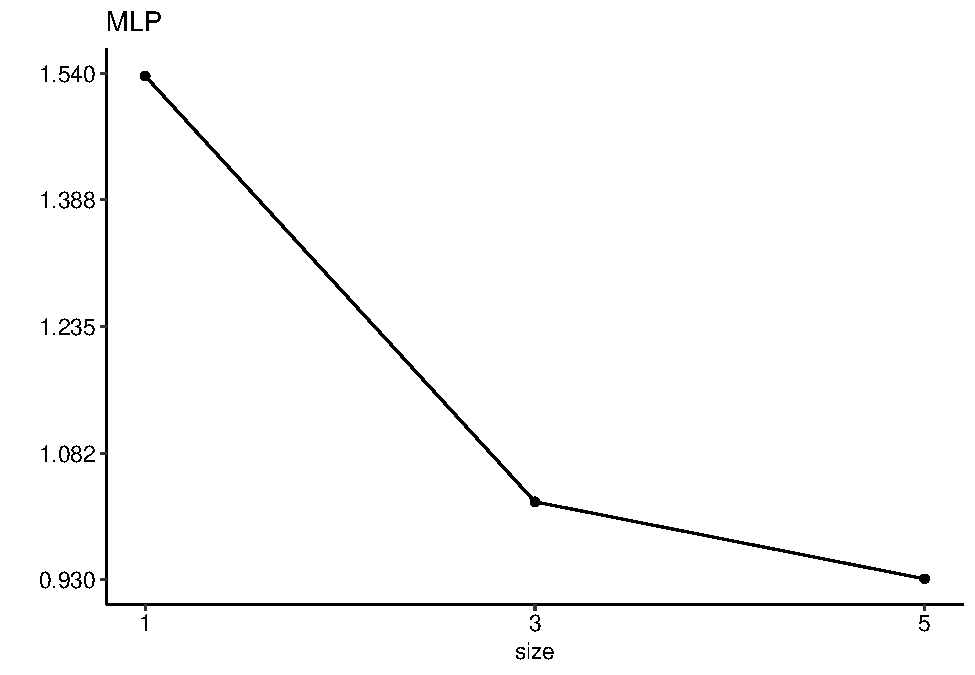
\includegraphics{sl-inf-cairs-2301_files/figure-latex/optResults-4.pdf}

\begin{Shaded}
\begin{Highlighting}[]
\NormalTok{df\_hp\_mlpwd}\OtherTok{\textless{}{-}}\NormalTok{fit\_06mlpWD}\SpecialCharTok{$}\NormalTok{results}
\NormalTok{df\_hp\_mlpwd}\SpecialCharTok{$}\NormalTok{decay}\OtherTok{\textless{}{-}}\FunctionTok{sprintf}\NormalTok{(}\StringTok{"\%.4f"}\NormalTok{,df\_hp\_mlpwd}\SpecialCharTok{$}\NormalTok{decay)}
\NormalTok{plt\_mlpwd}\OtherTok{\textless{}{-}}\FunctionTok{ggplot}\NormalTok{(}\AttributeTok{data=}\NormalTok{df\_hp\_mlpwd,}
                \FunctionTok{aes}\NormalTok{(}\AttributeTok{y =}\NormalTok{ logLoss, }\AttributeTok{x =}\NormalTok{ size,}\AttributeTok{color=}\NormalTok{decay)) }\SpecialCharTok{+}
  \FunctionTok{geom\_point}\NormalTok{() }\SpecialCharTok{+} \FunctionTok{geom\_line}\NormalTok{() }\SpecialCharTok{+} \FunctionTok{theme\_classic}\NormalTok{()}\SpecialCharTok{+}
  \CommentTok{\# facet\_wrap(. \textasciitilde{}epsilon, ncol = 3,labeller =label\_both)+}
  \FunctionTok{labs}\NormalTok{(}\AttributeTok{color=}\StringTok{"decay"}\NormalTok{,}\AttributeTok{x=}\StringTok{"size"}\NormalTok{,}\AttributeTok{y=}\StringTok{""}\NormalTok{) }\SpecialCharTok{+}
  \FunctionTok{ggtitle}\NormalTok{(}\StringTok{"MLP{-}WD"}\NormalTok{)}\SpecialCharTok{+}
  \FunctionTok{theme}\NormalTok{(}\AttributeTok{legend.position =} \StringTok{"right"}\NormalTok{,}
        \AttributeTok{axis.title =} \FunctionTok{element\_text}\NormalTok{(}\AttributeTok{face =} \StringTok{"plain"}\NormalTok{,}\AttributeTok{size =} \DecValTok{11}\NormalTok{,}\AttributeTok{color =} \StringTok{"black"}\NormalTok{),}
        \AttributeTok{axis.text =} \FunctionTok{element\_text}\NormalTok{(}\AttributeTok{face =} \StringTok{"plain"}\NormalTok{,}\AttributeTok{size =} \DecValTok{11}\NormalTok{,}\AttributeTok{color =} \StringTok{"black"}\NormalTok{),}
        \AttributeTok{strip.text =} \FunctionTok{element\_text}\NormalTok{(}\AttributeTok{face =} \StringTok{"plain"}\NormalTok{,}\AttributeTok{size =} \DecValTok{11}\NormalTok{),}
        \AttributeTok{legend.title =} \FunctionTok{element\_text}\NormalTok{(}\AttributeTok{face =} \StringTok{"plain"}\NormalTok{,}\AttributeTok{size =} \DecValTok{11}\NormalTok{),}
        \AttributeTok{legend.text =} \FunctionTok{element\_text}\NormalTok{(}\AttributeTok{face =} \StringTok{"plain"}\NormalTok{,}\AttributeTok{size =} \DecValTok{11}\NormalTok{),}
        \AttributeTok{panel.spacing =} \FunctionTok{unit}\NormalTok{(}\DecValTok{1}\NormalTok{, }\StringTok{"lines"}\NormalTok{))}\SpecialCharTok{+}
  \FunctionTok{scale\_x\_continuous}\NormalTok{(}\AttributeTok{breaks =} \FunctionTok{c}\NormalTok{(}\DecValTok{1}\NormalTok{,}\DecValTok{3}\NormalTok{,}\FloatTok{5.0}\NormalTok{))}\SpecialCharTok{+}
  \FunctionTok{scale\_y\_continuous}\NormalTok{(}\AttributeTok{breaks =} \FunctionTok{round}\NormalTok{(}\FunctionTok{seq}\NormalTok{(}\FloatTok{0.75}\NormalTok{,}\FloatTok{1.54}\NormalTok{,}\AttributeTok{length.out=}\DecValTok{5}\NormalTok{),}\DecValTok{3}\NormalTok{)}
\NormalTok{                     ,}\AttributeTok{limits =} \FunctionTok{c}\NormalTok{(}\FloatTok{0.75}\NormalTok{,}\FloatTok{1.54}\NormalTok{))}
\NormalTok{plt\_mlpwd}
\end{Highlighting}
\end{Shaded}

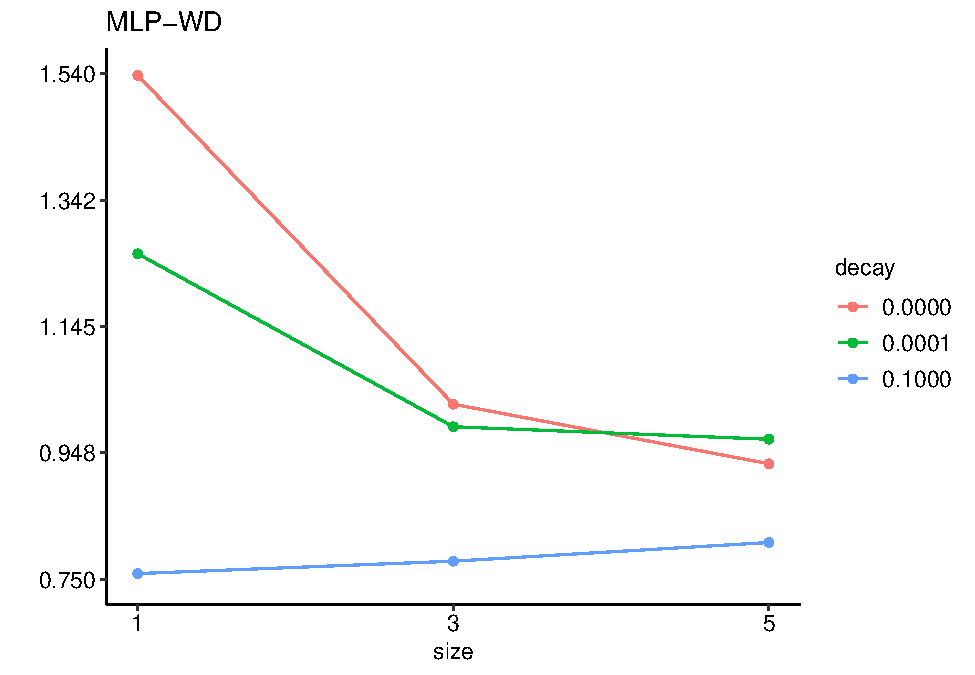
\includegraphics{sl-inf-cairs-2301_files/figure-latex/optResults-5.pdf}

\begin{Shaded}
\begin{Highlighting}[]
\NormalTok{df\_hp\_mlpD}\OtherTok{\textless{}{-}}\NormalTok{fit\_07mlpKerasDropout}\SpecialCharTok{$}\NormalTok{results}
\NormalTok{df\_hp\_mlpD}\SpecialCharTok{$}\NormalTok{dropout}\OtherTok{\textless{}{-}}\FunctionTok{sprintf}\NormalTok{(}\StringTok{"\%.2f"}\NormalTok{,df\_hp\_mlpD}\SpecialCharTok{$}\NormalTok{dropout)}
\NormalTok{plt\_mlpD}\OtherTok{\textless{}{-}}\FunctionTok{ggplot}\NormalTok{(}\AttributeTok{data=}\NormalTok{df\_hp\_mlpD,}
                \FunctionTok{aes}\NormalTok{(}\AttributeTok{y =}\NormalTok{ logLoss, }\AttributeTok{x =}\NormalTok{ size,}\AttributeTok{color=}\NormalTok{dropout)) }\SpecialCharTok{+}
  \FunctionTok{geom\_point}\NormalTok{() }\SpecialCharTok{+} \FunctionTok{geom\_line}\NormalTok{() }\SpecialCharTok{+} \FunctionTok{theme\_classic}\NormalTok{()}\SpecialCharTok{+}
  \CommentTok{\# facet\_wrap(. \textasciitilde{}epsilon, ncol = 3,labeller =label\_both)+}
  \FunctionTok{labs}\NormalTok{(}\AttributeTok{color=}\StringTok{"dropout"}\NormalTok{,}\AttributeTok{x=}\StringTok{"size"}\NormalTok{,}\AttributeTok{y=}\StringTok{""}\NormalTok{) }\SpecialCharTok{+}
  \FunctionTok{ggtitle}\NormalTok{(}\StringTok{"MLP{-}D"}\NormalTok{)}\SpecialCharTok{+}
  \FunctionTok{theme}\NormalTok{(}\AttributeTok{legend.position =} \StringTok{"right"}\NormalTok{,}
        \AttributeTok{axis.title =} \FunctionTok{element\_text}\NormalTok{(}\AttributeTok{face =} \StringTok{"plain"}\NormalTok{,}\AttributeTok{size =} \DecValTok{11}\NormalTok{,}\AttributeTok{color =} \StringTok{"black"}\NormalTok{),}
        \AttributeTok{axis.text =} \FunctionTok{element\_text}\NormalTok{(}\AttributeTok{face =} \StringTok{"plain"}\NormalTok{,}\AttributeTok{size =} \DecValTok{11}\NormalTok{,}\AttributeTok{color =} \StringTok{"black"}\NormalTok{),}
        \AttributeTok{strip.text =} \FunctionTok{element\_text}\NormalTok{(}\AttributeTok{face =} \StringTok{"plain"}\NormalTok{,}\AttributeTok{size =} \DecValTok{11}\NormalTok{),}
        \AttributeTok{legend.title =} \FunctionTok{element\_text}\NormalTok{(}\AttributeTok{face =} \StringTok{"plain"}\NormalTok{,}\AttributeTok{size =} \DecValTok{11}\NormalTok{),}
        \AttributeTok{legend.text =} \FunctionTok{element\_text}\NormalTok{(}\AttributeTok{face =} \StringTok{"plain"}\NormalTok{,}\AttributeTok{size =} \DecValTok{11}\NormalTok{),}
        \AttributeTok{panel.spacing =} \FunctionTok{unit}\NormalTok{(}\DecValTok{1}\NormalTok{, }\StringTok{"lines"}\NormalTok{))}\SpecialCharTok{+}
  \FunctionTok{scale\_x\_continuous}\NormalTok{(}\AttributeTok{breaks =} \FunctionTok{c}\NormalTok{(}\DecValTok{1}\NormalTok{,}\DecValTok{3}\NormalTok{,}\DecValTok{5}\NormalTok{))}\SpecialCharTok{+}
  \FunctionTok{scale\_y\_continuous}\NormalTok{(}\AttributeTok{breaks =} \FunctionTok{round}\NormalTok{(}\FunctionTok{seq}\NormalTok{(}\FloatTok{2.235}\NormalTok{,}\FloatTok{2.41}\NormalTok{,}\AttributeTok{length.out=}\DecValTok{5}\NormalTok{),}\DecValTok{3}\NormalTok{),}
                     \AttributeTok{limits =} \FunctionTok{c}\NormalTok{(}\FloatTok{2.235}\NormalTok{,}\FloatTok{2.41}\NormalTok{))}
\NormalTok{plt\_mlpD}
\end{Highlighting}
\end{Shaded}

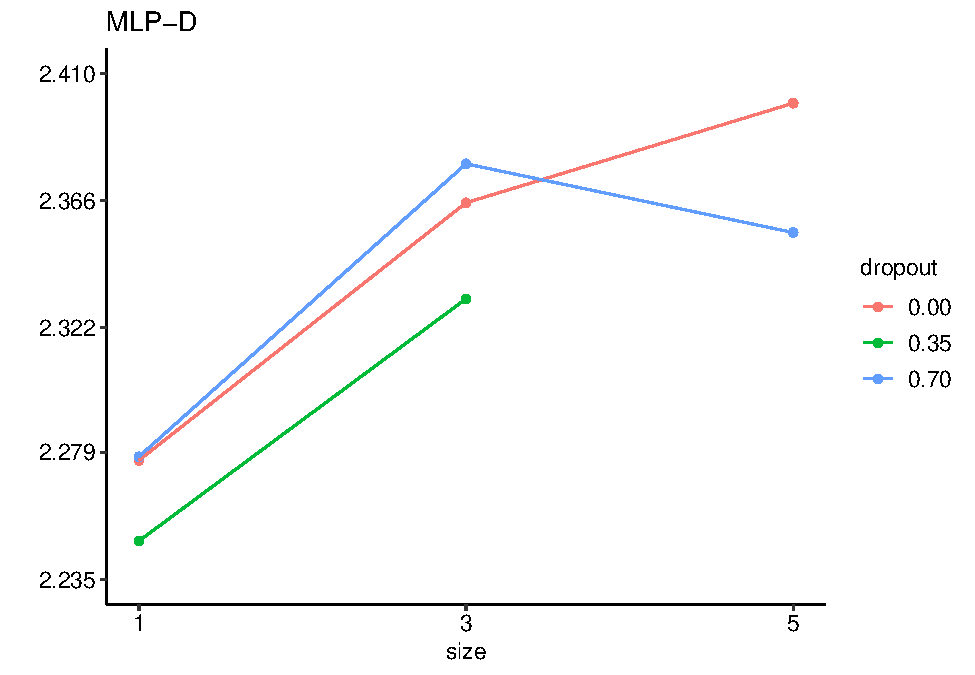
\includegraphics{sl-inf-cairs-2301_files/figure-latex/optResults-6.pdf}

\begin{Shaded}
\begin{Highlighting}[]
\NormalTok{df\_hp\_svmp}\OtherTok{\textless{}{-}}\NormalTok{fit\_09svmp}\SpecialCharTok{$}\NormalTok{results}
\NormalTok{df\_hp\_svmp}\SpecialCharTok{$}\NormalTok{scale}\OtherTok{\textless{}{-}}\FunctionTok{sprintf}\NormalTok{(}\StringTok{"\%.3f"}\NormalTok{,df\_hp\_svmp}\SpecialCharTok{$}\NormalTok{scale)}
\NormalTok{plt\_svmp}\OtherTok{\textless{}{-}}\FunctionTok{ggplot}\NormalTok{(}\AttributeTok{data=}\NormalTok{df\_hp\_svmp,}
                \FunctionTok{aes}\NormalTok{(}\AttributeTok{y =}\NormalTok{ logLoss, }\AttributeTok{x =}\NormalTok{ degree,}\AttributeTok{color=}\NormalTok{scale)) }\SpecialCharTok{+}
  \FunctionTok{geom\_point}\NormalTok{() }\SpecialCharTok{+} \FunctionTok{geom\_line}\NormalTok{() }\SpecialCharTok{+} \FunctionTok{theme\_classic}\NormalTok{()}\SpecialCharTok{+}
  \FunctionTok{facet\_wrap}\NormalTok{(. }\SpecialCharTok{\textasciitilde{}}\NormalTok{C, }\AttributeTok{ncol =} \DecValTok{3}\NormalTok{,}\AttributeTok{labeller =}\NormalTok{label\_both,}\AttributeTok{scales =} \StringTok{"fixed"}\NormalTok{)}\SpecialCharTok{+}
  \FunctionTok{labs}\NormalTok{(}\AttributeTok{color=}\StringTok{"scale"}\NormalTok{,}\AttributeTok{x=}\StringTok{"Polynomial degree"}\NormalTok{,}\AttributeTok{y=}\StringTok{""}\NormalTok{) }\SpecialCharTok{+}
  \FunctionTok{ggtitle}\NormalTok{(}\StringTok{"SVM{-}P"}\NormalTok{)}\SpecialCharTok{+}
  \FunctionTok{theme}\NormalTok{(}\AttributeTok{legend.position =} \StringTok{"right"}\NormalTok{,}
        \AttributeTok{axis.title =} \FunctionTok{element\_text}\NormalTok{(}\AttributeTok{face =} \StringTok{"plain"}\NormalTok{,}\AttributeTok{size =} \DecValTok{11}\NormalTok{,}\AttributeTok{color =} \StringTok{"black"}\NormalTok{),}
        \AttributeTok{axis.text =} \FunctionTok{element\_text}\NormalTok{(}\AttributeTok{face =} \StringTok{"plain"}\NormalTok{,}\AttributeTok{size =} \DecValTok{11}\NormalTok{,}\AttributeTok{color =} \StringTok{"black"}\NormalTok{),}
        \AttributeTok{strip.text =} \FunctionTok{element\_text}\NormalTok{(}\AttributeTok{face =} \StringTok{"plain"}\NormalTok{,}\AttributeTok{size =} \DecValTok{11}\NormalTok{),}
        \AttributeTok{legend.title =} \FunctionTok{element\_text}\NormalTok{(}\AttributeTok{face =} \StringTok{"plain"}\NormalTok{,}\AttributeTok{size =} \DecValTok{11}\NormalTok{),}
        \AttributeTok{legend.text =} \FunctionTok{element\_text}\NormalTok{(}\AttributeTok{face =} \StringTok{"plain"}\NormalTok{,}\AttributeTok{size =} \DecValTok{11}\NormalTok{),}
        \AttributeTok{panel.spacing =} \FunctionTok{unit}\NormalTok{(}\DecValTok{1}\NormalTok{, }\StringTok{"lines"}\NormalTok{))}\SpecialCharTok{+}
  \FunctionTok{scale\_x\_continuous}\NormalTok{(}\AttributeTok{breaks =} \FunctionTok{c}\NormalTok{(}\DecValTok{1}\NormalTok{,}\DecValTok{2}\NormalTok{,}\DecValTok{3}\NormalTok{))}\SpecialCharTok{+}
  \FunctionTok{scale\_y\_continuous}\NormalTok{(}\AttributeTok{breaks =} \FunctionTok{round}\NormalTok{(}\FunctionTok{seq}\NormalTok{(}\FloatTok{1.166}\NormalTok{,}\FloatTok{1.379}\NormalTok{,}\AttributeTok{length.out=}\DecValTok{5}\NormalTok{),}\DecValTok{3}\NormalTok{),}
                     \AttributeTok{limits =} \FunctionTok{c}\NormalTok{(}\FloatTok{1.166}\NormalTok{,}\FloatTok{1.379}\NormalTok{))}
\NormalTok{plt\_svmp}
\end{Highlighting}
\end{Shaded}

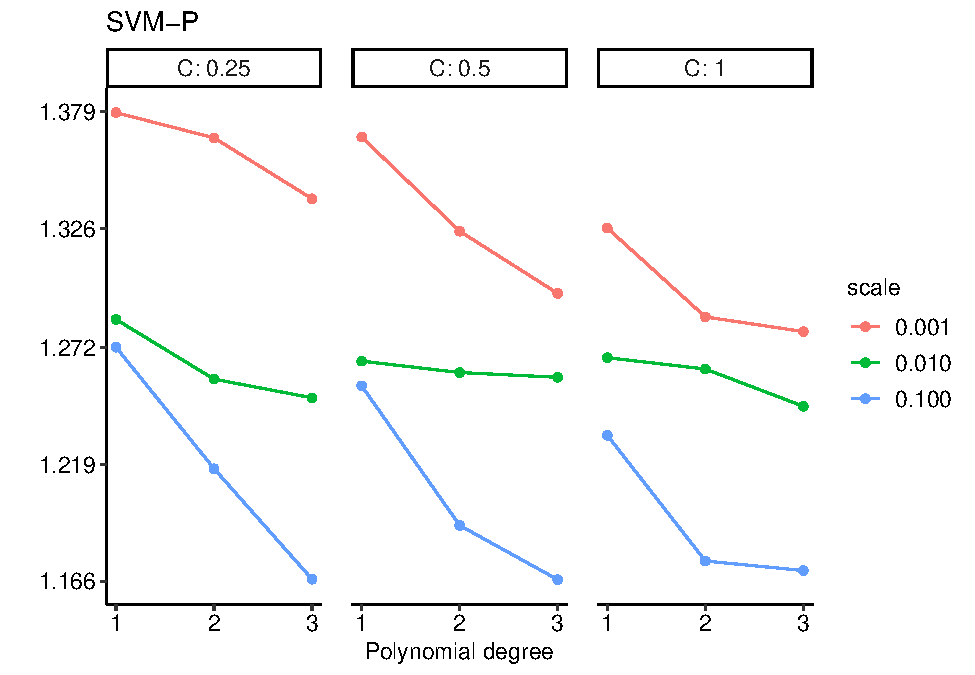
\includegraphics{sl-inf-cairs-2301_files/figure-latex/optResults-7.pdf}

\begin{Shaded}
\begin{Highlighting}[]
\CommentTok{\# df\_hp\_svmr\textless{}{-}fit\_10svmr$results}
\CommentTok{\# df\_hp\_svmr$C\textless{}{-}factor(sprintf("\%.2f",df\_hp\_svmr$C))}
\NormalTok{plt\_svmr}\OtherTok{\textless{}{-}}\FunctionTok{ggplot}\NormalTok{(}\AttributeTok{data=}\NormalTok{fit\_10svmr}\SpecialCharTok{$}\NormalTok{results,}
                \FunctionTok{aes}\NormalTok{(}\AttributeTok{y =}\NormalTok{ logLoss, }\AttributeTok{x =}\NormalTok{ C)) }\SpecialCharTok{+}
  \FunctionTok{geom\_point}\NormalTok{() }\SpecialCharTok{+} \FunctionTok{geom\_line}\NormalTok{() }\SpecialCharTok{+} \FunctionTok{theme\_classic}\NormalTok{()}\SpecialCharTok{+}
  \CommentTok{\# facet\_wrap(. \textasciitilde{}degree, ncol = 3,labeller =label\_both)+}
  \FunctionTok{labs}\NormalTok{(}\AttributeTok{color=}\StringTok{""}\NormalTok{,}\AttributeTok{x=}\StringTok{"cost"}\NormalTok{,}\AttributeTok{y=}\StringTok{""}\NormalTok{) }\SpecialCharTok{+}
  \FunctionTok{ggtitle}\NormalTok{(}\StringTok{"SVM{-}R"}\NormalTok{)}\SpecialCharTok{+}
  \FunctionTok{theme}\NormalTok{(}\AttributeTok{legend.position =} \StringTok{"right"}\NormalTok{,}
        \AttributeTok{axis.title =} \FunctionTok{element\_text}\NormalTok{(}\AttributeTok{face =} \StringTok{"plain"}\NormalTok{,}\AttributeTok{size =} \DecValTok{11}\NormalTok{,}\AttributeTok{color =} \StringTok{"black"}\NormalTok{),}
        \AttributeTok{axis.text =} \FunctionTok{element\_text}\NormalTok{(}\AttributeTok{face =} \StringTok{"plain"}\NormalTok{,}\AttributeTok{size =} \DecValTok{11}\NormalTok{,}\AttributeTok{color =} \StringTok{"black"}\NormalTok{),}
        \AttributeTok{strip.text =} \FunctionTok{element\_text}\NormalTok{(}\AttributeTok{face =} \StringTok{"plain"}\NormalTok{,}\AttributeTok{size =} \DecValTok{11}\NormalTok{),}
        \AttributeTok{legend.title =} \FunctionTok{element\_text}\NormalTok{(}\AttributeTok{face =} \StringTok{"plain"}\NormalTok{,}\AttributeTok{size =} \DecValTok{11}\NormalTok{),}
        \AttributeTok{legend.text =} \FunctionTok{element\_text}\NormalTok{(}\AttributeTok{face =} \StringTok{"plain"}\NormalTok{,}\AttributeTok{size =} \DecValTok{11}\NormalTok{),}
        \AttributeTok{panel.spacing =} \FunctionTok{unit}\NormalTok{(}\DecValTok{1}\NormalTok{, }\StringTok{"lines"}\NormalTok{))}\SpecialCharTok{+}
  \FunctionTok{scale\_x\_continuous}\NormalTok{(}\AttributeTok{breaks =} \FunctionTok{c}\NormalTok{(.}\DecValTok{25}\NormalTok{,.}\DecValTok{5}\NormalTok{,}\DecValTok{1}\NormalTok{))}\SpecialCharTok{+}
  \FunctionTok{scale\_y\_continuous}\NormalTok{(}\AttributeTok{breaks =} \FunctionTok{round}\NormalTok{(}\FunctionTok{seq}\NormalTok{(}\FloatTok{1.0930}\NormalTok{,}\FloatTok{1.1051}\NormalTok{,}\AttributeTok{length.out=}\DecValTok{5}\NormalTok{),}\DecValTok{3}\NormalTok{),}
                     \AttributeTok{limits =} \FunctionTok{c}\NormalTok{(}\FloatTok{1.0930}\NormalTok{,}\FloatTok{1.1051}\NormalTok{))}
\NormalTok{plt\_svmr}
\end{Highlighting}
\end{Shaded}

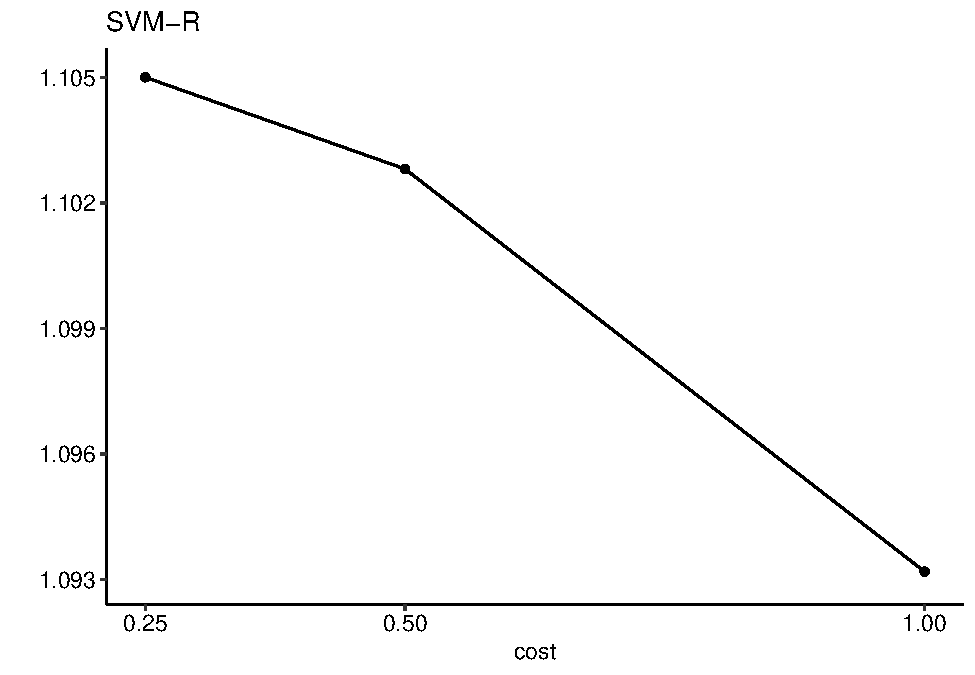
\includegraphics{sl-inf-cairs-2301_files/figure-latex/optResults-8.pdf}

\begin{Shaded}
\begin{Highlighting}[]
\CommentTok{\# df\_hp\_svmr\textless{}{-}fit\_10svmr$results}
\CommentTok{\# df\_hp\_svmr$C\textless{}{-}factor(sprintf("\%.2f",df\_hp\_svmr$C))}
\NormalTok{plt\_cart}\OtherTok{\textless{}{-}}\FunctionTok{ggplot}\NormalTok{(}\AttributeTok{data=}\NormalTok{fit\_11cart}\SpecialCharTok{$}\NormalTok{results,}
                \FunctionTok{aes}\NormalTok{(}\AttributeTok{y =}\NormalTok{ logLoss, }\AttributeTok{x =}\NormalTok{ maxdepth)) }\SpecialCharTok{+}
  \FunctionTok{geom\_point}\NormalTok{() }\SpecialCharTok{+} \FunctionTok{geom\_line}\NormalTok{() }\SpecialCharTok{+} \FunctionTok{theme\_classic}\NormalTok{()}\SpecialCharTok{+}
  \CommentTok{\# facet\_wrap(. \textasciitilde{}degree, ncol = 3,labeller =label\_both)+}
  \FunctionTok{labs}\NormalTok{(}\AttributeTok{color=}\StringTok{""}\NormalTok{,}\AttributeTok{x=}\StringTok{"maxdepth"}\NormalTok{,}\AttributeTok{y=}\StringTok{""}\NormalTok{) }\SpecialCharTok{+}
  \FunctionTok{ggtitle}\NormalTok{(}\StringTok{"CART"}\NormalTok{)}\SpecialCharTok{+}
  \FunctionTok{theme}\NormalTok{(}\AttributeTok{legend.position =} \StringTok{"right"}\NormalTok{,}
        \AttributeTok{axis.title =} \FunctionTok{element\_text}\NormalTok{(}\AttributeTok{face =} \StringTok{"plain"}\NormalTok{,}\AttributeTok{size =} \DecValTok{11}\NormalTok{,}\AttributeTok{color =} \StringTok{"black"}\NormalTok{),}
        \AttributeTok{axis.text =} \FunctionTok{element\_text}\NormalTok{(}\AttributeTok{face =} \StringTok{"plain"}\NormalTok{,}\AttributeTok{size =} \DecValTok{11}\NormalTok{,}\AttributeTok{color =} \StringTok{"black"}\NormalTok{),}
        \AttributeTok{strip.text =} \FunctionTok{element\_text}\NormalTok{(}\AttributeTok{face =} \StringTok{"plain"}\NormalTok{,}\AttributeTok{size =} \DecValTok{11}\NormalTok{),}
        \AttributeTok{legend.title =} \FunctionTok{element\_text}\NormalTok{(}\AttributeTok{face =} \StringTok{"plain"}\NormalTok{,}\AttributeTok{size =} \DecValTok{11}\NormalTok{),}
        \AttributeTok{legend.text =} \FunctionTok{element\_text}\NormalTok{(}\AttributeTok{face =} \StringTok{"plain"}\NormalTok{,}\AttributeTok{size =} \DecValTok{11}\NormalTok{),}
        \AttributeTok{panel.spacing =} \FunctionTok{unit}\NormalTok{(}\DecValTok{1}\NormalTok{, }\StringTok{"lines"}\NormalTok{))}\SpecialCharTok{+}
  \FunctionTok{scale\_x\_continuous}\NormalTok{(}\AttributeTok{breaks =} \FunctionTok{c}\NormalTok{(}\DecValTok{1}\NormalTok{,}\DecValTok{2}\NormalTok{,}\DecValTok{3}\NormalTok{))}\SpecialCharTok{+}
  \FunctionTok{scale\_y\_continuous}\NormalTok{(}\AttributeTok{breaks =} \FunctionTok{round}\NormalTok{(}\FunctionTok{seq}\NormalTok{(.}\DecValTok{995}\NormalTok{,}\FloatTok{1.35}\NormalTok{,}\AttributeTok{length.out=}\DecValTok{5}\NormalTok{),}\DecValTok{3}\NormalTok{)}
\NormalTok{                     ,}\AttributeTok{limits =} \FunctionTok{c}\NormalTok{(}\FloatTok{0.995}\NormalTok{,}\FloatTok{1.35}\NormalTok{))}
\NormalTok{plt\_cart}
\end{Highlighting}
\end{Shaded}

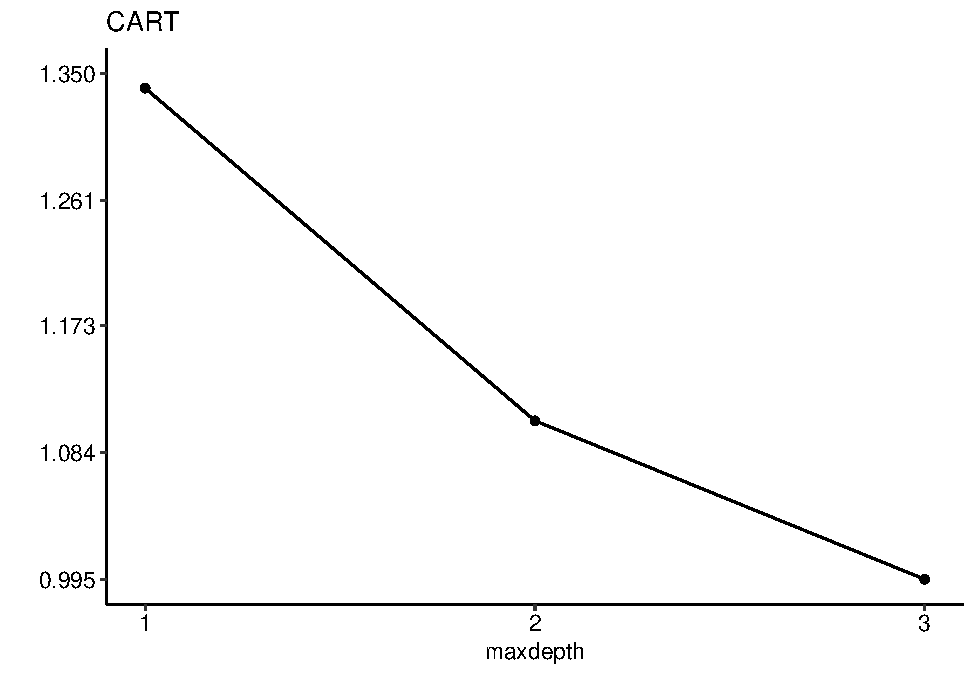
\includegraphics{sl-inf-cairs-2301_files/figure-latex/optResults-9.pdf}

\begin{Shaded}
\begin{Highlighting}[]
\CommentTok{\# df\_hp\_svmr\textless{}{-}fit\_10svmr$results}
\CommentTok{\# df\_hp\_svmr$C\textless{}{-}factor(sprintf("\%.2f",df\_hp\_svmr$C))}
\NormalTok{plt\_rf}\OtherTok{\textless{}{-}}\FunctionTok{ggplot}\NormalTok{(}\AttributeTok{data=}\NormalTok{fit\_13rf}\SpecialCharTok{$}\NormalTok{results,}
                \FunctionTok{aes}\NormalTok{(}\AttributeTok{y =}\NormalTok{ logLoss, }\AttributeTok{x =}\NormalTok{ mtry)) }\SpecialCharTok{+}
  \FunctionTok{geom\_point}\NormalTok{() }\SpecialCharTok{+} \FunctionTok{geom\_line}\NormalTok{() }\SpecialCharTok{+} \FunctionTok{theme\_classic}\NormalTok{()}\SpecialCharTok{+}
  \CommentTok{\# facet\_wrap(. \textasciitilde{}degree, ncol = 3,labeller =label\_both)+}
  \FunctionTok{labs}\NormalTok{(}\AttributeTok{color=}\StringTok{""}\NormalTok{,}\AttributeTok{x=}\StringTok{"mtry"}\NormalTok{,}\AttributeTok{y=}\StringTok{""}\NormalTok{) }\SpecialCharTok{+}
  \FunctionTok{ggtitle}\NormalTok{(}\StringTok{"RF"}\NormalTok{)}\SpecialCharTok{+}
  \FunctionTok{theme}\NormalTok{(}\AttributeTok{legend.position =} \StringTok{"right"}\NormalTok{,}
        \AttributeTok{axis.title =} \FunctionTok{element\_text}\NormalTok{(}\AttributeTok{face =} \StringTok{"plain"}\NormalTok{,}\AttributeTok{size =} \DecValTok{11}\NormalTok{,}\AttributeTok{color =} \StringTok{"black"}\NormalTok{),}
        \AttributeTok{axis.text =} \FunctionTok{element\_text}\NormalTok{(}\AttributeTok{face =} \StringTok{"plain"}\NormalTok{,}\AttributeTok{size =} \DecValTok{11}\NormalTok{,}\AttributeTok{color =} \StringTok{"black"}\NormalTok{),}
        \AttributeTok{strip.text =} \FunctionTok{element\_text}\NormalTok{(}\AttributeTok{face =} \StringTok{"plain"}\NormalTok{,}\AttributeTok{size =} \DecValTok{11}\NormalTok{),}
        \AttributeTok{legend.title =} \FunctionTok{element\_text}\NormalTok{(}\AttributeTok{face =} \StringTok{"plain"}\NormalTok{,}\AttributeTok{size =} \DecValTok{11}\NormalTok{),}
        \AttributeTok{legend.text =} \FunctionTok{element\_text}\NormalTok{(}\AttributeTok{face =} \StringTok{"plain"}\NormalTok{,}\AttributeTok{size =} \DecValTok{11}\NormalTok{),}
        \AttributeTok{panel.spacing =} \FunctionTok{unit}\NormalTok{(}\DecValTok{1}\NormalTok{, }\StringTok{"lines"}\NormalTok{))}\SpecialCharTok{+}
  \FunctionTok{scale\_x\_continuous}\NormalTok{(}\AttributeTok{breaks =} \FunctionTok{c}\NormalTok{(}\DecValTok{2}\NormalTok{,}\DecValTok{6}\NormalTok{,}\DecValTok{10}\NormalTok{))}\SpecialCharTok{+}
  \FunctionTok{scale\_y\_continuous}\NormalTok{(}\AttributeTok{breaks =} \FunctionTok{round}\NormalTok{(}\FunctionTok{seq}\NormalTok{(}\FloatTok{0.360}\NormalTok{,.}\DecValTok{387}\NormalTok{,}\AttributeTok{length.out=}\DecValTok{5}\NormalTok{),}\DecValTok{3}\NormalTok{),}
                     \AttributeTok{limits =} \FunctionTok{c}\NormalTok{(}\FloatTok{0.360}\NormalTok{,.}\DecValTok{387}\NormalTok{))}
\NormalTok{plt\_rf}
\end{Highlighting}
\end{Shaded}

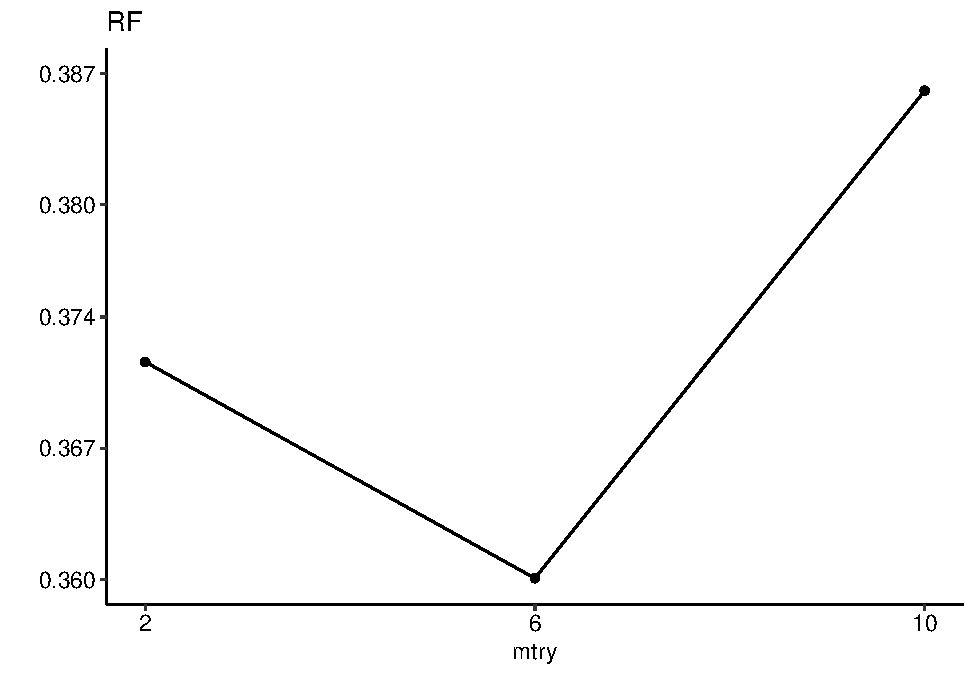
\includegraphics{sl-inf-cairs-2301_files/figure-latex/optResults-10.pdf}

\begin{Shaded}
\begin{Highlighting}[]
\NormalTok{plt\_layout\_matrix }\OtherTok{=} \FunctionTok{rbind}\NormalTok{(}\FunctionTok{c}\NormalTok{(}\DecValTok{3}\NormalTok{,}\DecValTok{2}\NormalTok{,}\DecValTok{2}\NormalTok{,}\DecValTok{1}\NormalTok{,}\DecValTok{1}\NormalTok{,}\DecValTok{1}\NormalTok{),}\FunctionTok{c}\NormalTok{(}\DecValTok{4}\NormalTok{,}\DecValTok{5}\NormalTok{,}\DecValTok{5}\NormalTok{,}\DecValTok{9}\NormalTok{,}\DecValTok{9}\NormalTok{,}\DecValTok{9}\NormalTok{),}
                          \FunctionTok{c}\NormalTok{(}\DecValTok{7}\NormalTok{,}\DecValTok{8}\NormalTok{,}\DecValTok{10}\NormalTok{,}\DecValTok{6}\NormalTok{,}\DecValTok{6}\NormalTok{,}\DecValTok{6}\NormalTok{))}
\NormalTok{plt\_hp\_all}\OtherTok{\textless{}{-}}\FunctionTok{arrangeGrob}\NormalTok{(}\AttributeTok{grobs=}\FunctionTok{list}\NormalTok{(plt\_rlr,plt\_glm,plt\_sda,plt\_mlp,}
\NormalTok{                        plt\_mlpD,plt\_mlpwd,plt\_cart,plt\_rf,}
\NormalTok{                        plt\_svmp,plt\_svmr),}\AttributeTok{nrow =}\DecValTok{3}\NormalTok{,}\AttributeTok{ncol=}\DecValTok{6}\NormalTok{,}
                        \AttributeTok{layout\_matrix =}\NormalTok{plt\_layout\_matrix)}
\NormalTok{plt\_hp\_all}\OtherTok{\textless{}{-}}\FunctionTok{grid.arrange}\NormalTok{(plt\_hp\_all)}
\end{Highlighting}
\end{Shaded}

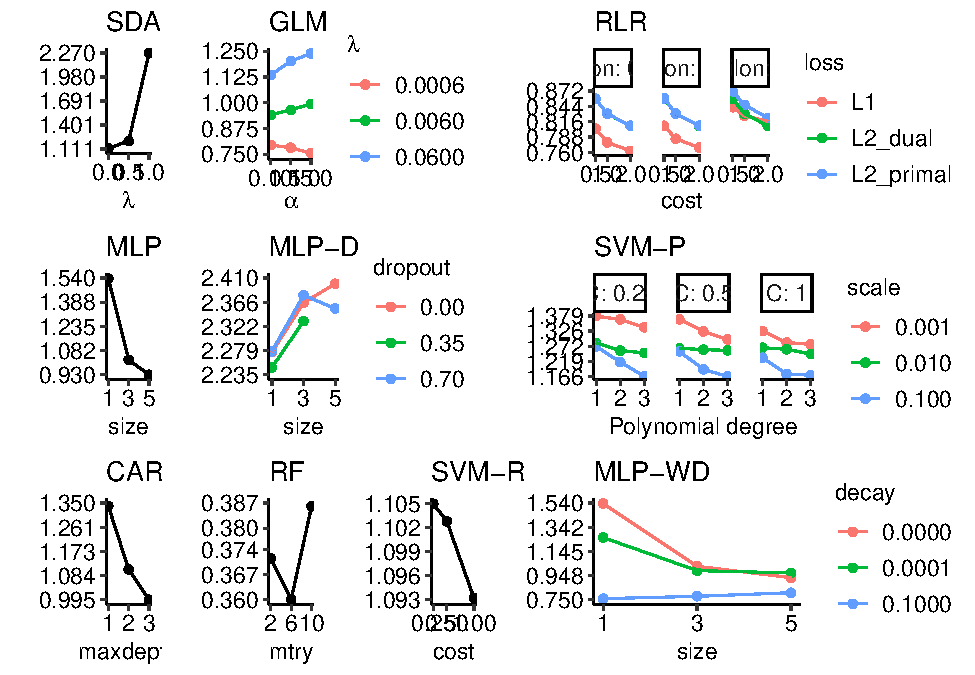
\includegraphics{sl-inf-cairs-2301_files/figure-latex/optResults-11.pdf}

\begin{Shaded}
\begin{Highlighting}[]
\NormalTok{plt\_hp\_all}\OtherTok{\textless{}{-}}\FunctionTok{annotate\_figure}\NormalTok{(}\AttributeTok{p =}\NormalTok{ plt\_hp\_all,}
                            \AttributeTok{left =} \FunctionTok{text\_grob}\NormalTok{(}\StringTok{"logLoss"}\NormalTok{, }\AttributeTok{face =} \StringTok{"plain"}\NormalTok{,}
                                             \AttributeTok{rot =} \DecValTok{90}\NormalTok{, }\AttributeTok{vjust =} \FloatTok{0.85}\NormalTok{),}
                            \AttributeTok{bottom =} \FunctionTok{text\_grob}\NormalTok{(}\StringTok{"Model hyperparameters"}\NormalTok{,}
                                               \AttributeTok{face =} \StringTok{"plain"}\NormalTok{, }\AttributeTok{vjust =} \FloatTok{0.45}\NormalTok{))}
\NormalTok{plt\_hp\_all}\OtherTok{\textless{}{-}}\NormalTok{ plt\_hp\_all}\SpecialCharTok{+}
  \FunctionTok{geom\_segment}\NormalTok{(}\FunctionTok{aes}\NormalTok{(}\AttributeTok{x =}\NormalTok{ .}\DecValTok{025}\NormalTok{, }\AttributeTok{y=}\FloatTok{0.03}\NormalTok{, }\AttributeTok{xend=}\FloatTok{0.025}\NormalTok{, }\AttributeTok{yend =}\NormalTok{ .}\DecValTok{98}\NormalTok{), }\AttributeTok{size =}\NormalTok{.}\DecValTok{6}\NormalTok{,}
               \AttributeTok{arrow =} \FunctionTok{arrow}\NormalTok{(}\AttributeTok{length =} \FunctionTok{unit}\NormalTok{(}\FloatTok{0.3}\NormalTok{, }\StringTok{"cm"}\NormalTok{))) }\SpecialCharTok{+}
  \FunctionTok{geom\_segment}\NormalTok{(}\FunctionTok{aes}\NormalTok{(}\AttributeTok{x =}\NormalTok{ .}\DecValTok{025}\NormalTok{, }\AttributeTok{y=}\FloatTok{0.03}\NormalTok{, }\AttributeTok{xend=}\FloatTok{0.98}\NormalTok{, }\AttributeTok{yend =}\NormalTok{ .}\DecValTok{03}\NormalTok{), }\AttributeTok{size =}\NormalTok{.}\DecValTok{6}\NormalTok{,}
               \AttributeTok{arrow =} \FunctionTok{arrow}\NormalTok{(}\AttributeTok{length =} \FunctionTok{unit}\NormalTok{(}\FloatTok{0.3}\NormalTok{, }\StringTok{"cm"}\NormalTok{)))}
\CommentTok{\# \#http://127.0.0.1:21067/graphics/plot\_zoom\_png?width=1257\&height=796}
\FunctionTok{ggsave}\NormalTok{(}\AttributeTok{filename =} \StringTok{"results/plt\_hp\_all.jpeg"}\NormalTok{,}\AttributeTok{plot =} \FunctionTok{last\_plot}\NormalTok{(),}
       \AttributeTok{device =} \StringTok{"jpeg"}\NormalTok{,}\AttributeTok{width =} \DecValTok{1257}\SpecialCharTok{/}\DecValTok{96}\NormalTok{,}\AttributeTok{height =} \DecValTok{796}\SpecialCharTok{/}\DecValTok{96}\NormalTok{,}\AttributeTok{dpi =} \DecValTok{600}\NormalTok{)}

\NormalTok{fit\_14xgb}\SpecialCharTok{$}\NormalTok{results}\SpecialCharTok{$}\NormalTok{max\_depth}\OtherTok{\textless{}{-}}\FunctionTok{as.factor}\NormalTok{(fit\_14xgb}\SpecialCharTok{$}\NormalTok{results}\SpecialCharTok{$}\NormalTok{max\_depth)}
\NormalTok{plt\_xgb}\OtherTok{\textless{}{-}}\FunctionTok{ggplot}\NormalTok{(}\AttributeTok{data=}\NormalTok{fit\_14xgb}\SpecialCharTok{$}\NormalTok{results,}
                \FunctionTok{aes}\NormalTok{(}\AttributeTok{y =}\NormalTok{ logLoss, }\AttributeTok{x =}\NormalTok{ nrounds, }\AttributeTok{color=}\NormalTok{max\_depth),}
                \AttributeTok{fill=}\NormalTok{max\_depth) }\SpecialCharTok{+}
  \FunctionTok{geom\_point}\NormalTok{(}\FunctionTok{aes}\NormalTok{(}\AttributeTok{colour =}\NormalTok{ max\_depth)) }\SpecialCharTok{+} \FunctionTok{geom\_line}\NormalTok{() }\SpecialCharTok{+}
  \FunctionTok{labs}\NormalTok{(}\AttributeTok{y=}\StringTok{""}\NormalTok{,}\AttributeTok{x=}\StringTok{""}\NormalTok{)}\SpecialCharTok{+}
  \FunctionTok{ggtitle}\NormalTok{(}\StringTok{"XGBoost"}\NormalTok{)}\SpecialCharTok{+}
  \FunctionTok{theme\_classic}\NormalTok{() }\SpecialCharTok{+}
  \FunctionTok{facet\_wrap}\NormalTok{(. }\SpecialCharTok{\textasciitilde{}}\NormalTok{colsample\_bytree}\SpecialCharTok{*}\NormalTok{eta}\SpecialCharTok{*}\NormalTok{subsample,}
             \AttributeTok{ncol =} \DecValTok{4}\NormalTok{,}\AttributeTok{labeller =}\NormalTok{label\_both )}\SpecialCharTok{+}
  \FunctionTok{theme}\NormalTok{(}\AttributeTok{legend.position =} \StringTok{"right"}\NormalTok{,}
        \AttributeTok{axis.title =} \FunctionTok{element\_text}\NormalTok{(}\AttributeTok{face =} \StringTok{"plain"}\NormalTok{,}\AttributeTok{size =} \DecValTok{11}\NormalTok{,}\AttributeTok{color =} \StringTok{"black"}\NormalTok{),}
        \AttributeTok{axis.text =} \FunctionTok{element\_text}\NormalTok{(}\AttributeTok{face =} \StringTok{"plain"}\NormalTok{,}\AttributeTok{size =} \DecValTok{11}\NormalTok{,}\AttributeTok{color =} \StringTok{"black"}\NormalTok{),}
        \AttributeTok{strip.text =} \FunctionTok{element\_text}\NormalTok{(}\AttributeTok{face =} \StringTok{"plain"}\NormalTok{,}\AttributeTok{size =} \DecValTok{11}\NormalTok{),}
        \AttributeTok{legend.title =} \FunctionTok{element\_text}\NormalTok{(}\AttributeTok{face =} \StringTok{"plain"}\NormalTok{,}\AttributeTok{size =} \DecValTok{11}\NormalTok{),}
        \AttributeTok{legend.text =} \FunctionTok{element\_text}\NormalTok{(}\AttributeTok{face =} \StringTok{"plain"}\NormalTok{,}\AttributeTok{size =} \DecValTok{11}\NormalTok{),}
        \AttributeTok{panel.spacing.x =} \FunctionTok{unit}\NormalTok{(}\DecValTok{1}\NormalTok{, }\StringTok{"lines"}\NormalTok{))}\SpecialCharTok{+}
  \FunctionTok{scale\_x\_continuous}\NormalTok{(}\AttributeTok{breaks =} \FunctionTok{c}\NormalTok{(}\DecValTok{50}\NormalTok{,}\DecValTok{100}\NormalTok{,}\DecValTok{150}\NormalTok{))}\SpecialCharTok{+}
  \FunctionTok{scale\_y\_continuous}\NormalTok{(}\AttributeTok{breaks =}\FunctionTok{round}\NormalTok{(}\FunctionTok{seq}\NormalTok{(}\FloatTok{0.360}\NormalTok{,}\FloatTok{0.756}\NormalTok{,}\AttributeTok{length.out=}\DecValTok{5}\NormalTok{),}\DecValTok{3}\NormalTok{),}
                     \AttributeTok{limits =} \FunctionTok{c}\NormalTok{(}\FloatTok{0.360}\NormalTok{,}\FloatTok{0.756}\NormalTok{))}
\NormalTok{plt\_xgb}
\end{Highlighting}
\end{Shaded}

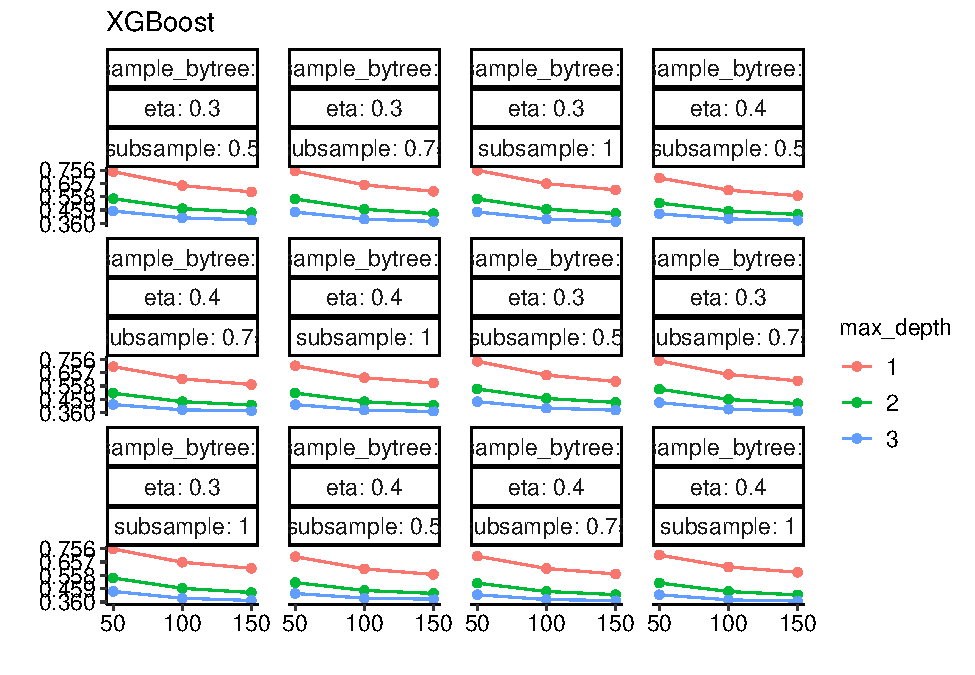
\includegraphics{sl-inf-cairs-2301_files/figure-latex/optResults-12.pdf}

\begin{Shaded}
\begin{Highlighting}[]
\NormalTok{plt\_xgb}\OtherTok{\textless{}{-}}\FunctionTok{annotate\_figure}\NormalTok{(}\AttributeTok{p =}\NormalTok{ plt\_xgb,}
                            \AttributeTok{left =} \FunctionTok{text\_grob}\NormalTok{(}\StringTok{"logLoss"}\NormalTok{, }\AttributeTok{face =} \StringTok{"plain"}\NormalTok{,}
                                             \AttributeTok{rot =} \DecValTok{90}\NormalTok{, }\AttributeTok{vjust =} \FloatTok{0.85}\NormalTok{),}
                            \AttributeTok{bottom =} \FunctionTok{text\_grob}\NormalTok{(}\StringTok{"nrounds"}\NormalTok{,}
                                               \AttributeTok{face =} \StringTok{"plain"}\NormalTok{, }\AttributeTok{vjust =} \FloatTok{0.45}\NormalTok{))}
\NormalTok{plt\_xgb}\OtherTok{\textless{}{-}}\NormalTok{ plt\_xgb}\SpecialCharTok{+}
  \FunctionTok{geom\_segment}\NormalTok{(}\FunctionTok{aes}\NormalTok{(}\AttributeTok{x =}\NormalTok{ .}\DecValTok{025}\NormalTok{, }\AttributeTok{y=}\FloatTok{0.03}\NormalTok{, }\AttributeTok{xend=}\FloatTok{0.025}\NormalTok{, }\AttributeTok{yend =}\NormalTok{ .}\DecValTok{98}\NormalTok{), }\AttributeTok{size =}\NormalTok{.}\DecValTok{6}\NormalTok{,}
               \AttributeTok{arrow =} \FunctionTok{arrow}\NormalTok{(}\AttributeTok{length =} \FunctionTok{unit}\NormalTok{(}\FloatTok{0.3}\NormalTok{, }\StringTok{"cm"}\NormalTok{))) }\SpecialCharTok{+}
  \FunctionTok{geom\_segment}\NormalTok{(}\FunctionTok{aes}\NormalTok{(}\AttributeTok{x =}\NormalTok{ .}\DecValTok{025}\NormalTok{, }\AttributeTok{y=}\FloatTok{0.03}\NormalTok{, }\AttributeTok{xend=}\FloatTok{0.98}\NormalTok{, }\AttributeTok{yend =}\NormalTok{ .}\DecValTok{03}\NormalTok{), }\AttributeTok{size =}\NormalTok{.}\DecValTok{6}\NormalTok{,}
               \AttributeTok{arrow =} \FunctionTok{arrow}\NormalTok{(}\AttributeTok{length =} \FunctionTok{unit}\NormalTok{(}\FloatTok{0.3}\NormalTok{, }\StringTok{"cm"}\NormalTok{)))}
\CommentTok{\# \#http://127.0.0.1:21067/graphics/plot\_zoom\_png?width=1257\&height=796}
\FunctionTok{ggsave}\NormalTok{(}\AttributeTok{filename =} \StringTok{"results/plt\_hp\_xgb.jpeg"}\NormalTok{,}\AttributeTok{plot =} \FunctionTok{last\_plot}\NormalTok{(),}
       \AttributeTok{device =} \StringTok{"jpeg"}\NormalTok{,}\AttributeTok{width =} \DecValTok{1257}\SpecialCharTok{/}\DecValTok{96}\NormalTok{,}\AttributeTok{height =} \DecValTok{796}\SpecialCharTok{/}\DecValTok{96}\NormalTok{,}\AttributeTok{dpi =} \DecValTok{600}\NormalTok{)}
\end{Highlighting}
\end{Shaded}

\begin{quote}
\hypertarget{nd-arrangement-of-hp-plots}{%
\subsubsection{2nd arrangement of hp
plots}\label{nd-arrangement-of-hp-plots}}
\end{quote}

\begin{Shaded}
\begin{Highlighting}[]
\NormalTok{plt\_layout\_matrix4 }\OtherTok{=} \FunctionTok{rbind}\NormalTok{(}\FunctionTok{c}\NormalTok{(}\DecValTok{1}\NormalTok{),}\FunctionTok{c}\NormalTok{(}\DecValTok{2}\NormalTok{,}\DecValTok{2}\NormalTok{,}\DecValTok{2}\NormalTok{,}\DecValTok{3}\NormalTok{,}\DecValTok{3}\NormalTok{),}\FunctionTok{c}\NormalTok{(}\DecValTok{4}\NormalTok{))}
\NormalTok{plt\_hp\_4}\OtherTok{\textless{}{-}}\FunctionTok{arrangeGrob}\NormalTok{(}
  \AttributeTok{grobs=} \FunctionTok{list}\NormalTok{(plt\_rlr,plt\_glm,plt\_sda,plt\_svmp),}
                         \AttributeTok{nrow =}\DecValTok{3}\NormalTok{,}\AttributeTok{ncol=}\DecValTok{4}\NormalTok{,}\AttributeTok{layout\_matrix =}\NormalTok{plt\_layout\_matrix4)}
\NormalTok{plt\_hp\_4}\OtherTok{\textless{}{-}}\FunctionTok{annotate\_figure}\NormalTok{(}\AttributeTok{p =}\NormalTok{ plt\_hp\_4,}
                            \AttributeTok{left =} \FunctionTok{text\_grob}\NormalTok{(}\StringTok{"logLoss"}\NormalTok{, }\AttributeTok{face =} \StringTok{"plain"}\NormalTok{,}
                                             \AttributeTok{rot =} \DecValTok{90}\NormalTok{, }\AttributeTok{vjust =} \FloatTok{0.25}\NormalTok{),}
                            \AttributeTok{bottom =} \FunctionTok{text\_grob}\NormalTok{(}\StringTok{"Model hyperparameters"}\NormalTok{,}
                                               \AttributeTok{face =} \StringTok{"plain"}\NormalTok{, }\AttributeTok{vjust =} \FloatTok{0.25}\NormalTok{))}
\NormalTok{plt\_hp\_4}\OtherTok{\textless{}{-}}\NormalTok{ plt\_hp\_4}\SpecialCharTok{+}
  \FunctionTok{geom\_segment}\NormalTok{(}\FunctionTok{aes}\NormalTok{(}\AttributeTok{x =}\NormalTok{ .}\DecValTok{04}\NormalTok{, }\AttributeTok{y=}\FloatTok{0.045}\NormalTok{, }\AttributeTok{xend=}\FloatTok{0.04}\NormalTok{, }\AttributeTok{yend =}\NormalTok{ .}\DecValTok{98}\NormalTok{), }\AttributeTok{size =}\NormalTok{.}\DecValTok{6}\NormalTok{,}
               \AttributeTok{arrow =} \FunctionTok{arrow}\NormalTok{(}\AttributeTok{length =} \FunctionTok{unit}\NormalTok{(}\FloatTok{0.3}\NormalTok{, }\StringTok{"cm"}\NormalTok{))) }\SpecialCharTok{+}
  \FunctionTok{geom\_segment}\NormalTok{(}\FunctionTok{aes}\NormalTok{(}\AttributeTok{x =}\NormalTok{ .}\DecValTok{04}\NormalTok{, }\AttributeTok{y=}\FloatTok{0.045}\NormalTok{, }\AttributeTok{xend=}\FloatTok{0.98}\NormalTok{, }\AttributeTok{yend =}\NormalTok{ .}\DecValTok{045}\NormalTok{), }\AttributeTok{size =}\NormalTok{.}\DecValTok{6}\NormalTok{,}
               \AttributeTok{arrow =} \FunctionTok{arrow}\NormalTok{(}\AttributeTok{length =} \FunctionTok{unit}\NormalTok{(}\FloatTok{0.3}\NormalTok{, }\StringTok{"cm"}\NormalTok{)))}
\NormalTok{plt\_hp\_4}\OtherTok{\textless{}{-}}\FunctionTok{grid.arrange}\NormalTok{(plt\_hp\_4)}
\end{Highlighting}
\end{Shaded}

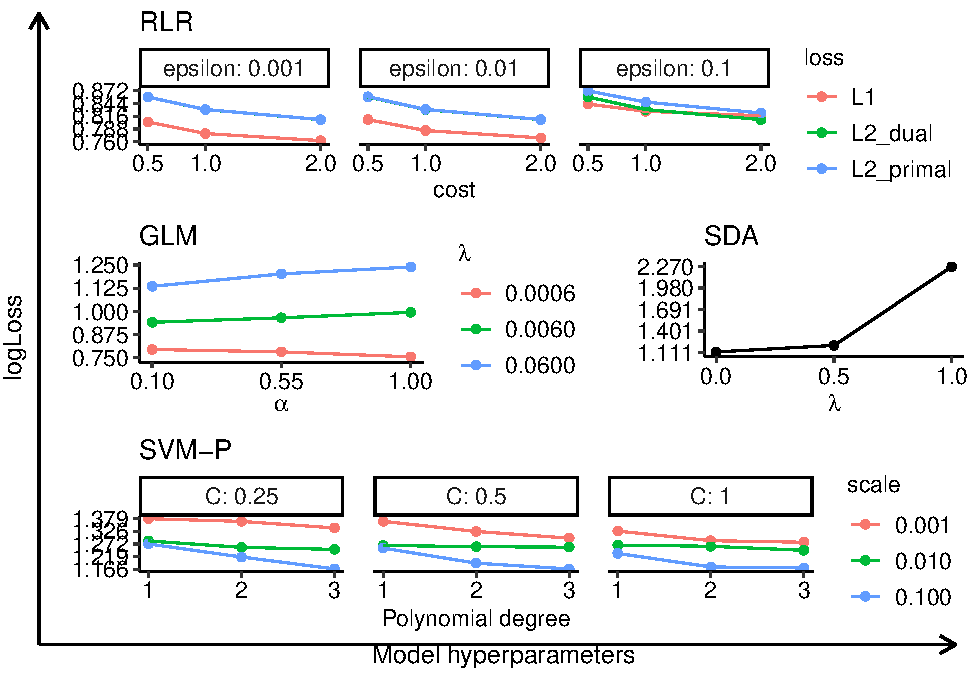
\includegraphics{sl-inf-cairs-2301_files/figure-latex/optResults2-1.pdf}

\begin{Shaded}
\begin{Highlighting}[]
\CommentTok{\# http://127.0.0.1:21067/graphics/plot\_zoom\_png?width=786\&height=605}
\FunctionTok{ggsave}\NormalTok{(}\AttributeTok{filename =} \StringTok{"results/plt\_hp\_4.jpeg"}\NormalTok{,}\AttributeTok{plot =} \FunctionTok{last\_plot}\NormalTok{(),}
       \AttributeTok{device =} \StringTok{"jpeg"}\NormalTok{,}\AttributeTok{height =} \DecValTok{605}\SpecialCharTok{/}\DecValTok{96}\NormalTok{,}\AttributeTok{width =} \DecValTok{786}\SpecialCharTok{/}\DecValTok{96}\NormalTok{,}\AttributeTok{dpi =} \DecValTok{600}\NormalTok{)}

\NormalTok{plt\_layout\_matrix5 }\OtherTok{=} \FunctionTok{rbind}\NormalTok{(}\FunctionTok{c}\NormalTok{(}\DecValTok{1}\NormalTok{,}\DecValTok{2}\NormalTok{),}\FunctionTok{c}\NormalTok{(}\DecValTok{3}\NormalTok{),}\FunctionTok{c}\NormalTok{(}\DecValTok{4}\NormalTok{),}\FunctionTok{c}\NormalTok{(}\DecValTok{5}\NormalTok{,}\DecValTok{6}\NormalTok{))}
\NormalTok{plt\_hp\_5}\OtherTok{\textless{}{-}}\FunctionTok{arrangeGrob}\NormalTok{(}
  \AttributeTok{grobs=} \FunctionTok{list}\NormalTok{(plt\_svmr,plt\_mlp,plt\_mlpwd,plt\_mlpD,plt\_cart,plt\_rf),}
                         \AttributeTok{nrow =}\DecValTok{4}\NormalTok{,}\AttributeTok{ncol=}\DecValTok{2}\NormalTok{,}\AttributeTok{layout\_matrix =}\NormalTok{plt\_layout\_matrix5)}
\NormalTok{plt\_hp\_5}\OtherTok{\textless{}{-}}\FunctionTok{annotate\_figure}\NormalTok{(}\AttributeTok{p =}\NormalTok{ plt\_hp\_5,}
                            \AttributeTok{left =} \FunctionTok{text\_grob}\NormalTok{(}\StringTok{"logLoss"}\NormalTok{, }\AttributeTok{face =} \StringTok{"plain"}\NormalTok{,}
                                             \AttributeTok{rot =} \DecValTok{90}\NormalTok{, }\AttributeTok{vjust =} \FloatTok{0.25}\NormalTok{),}
                            \AttributeTok{bottom =} \FunctionTok{text\_grob}\NormalTok{(}\StringTok{"Model hyperparameters"}\NormalTok{,}
                                               \AttributeTok{face =} \StringTok{"plain"}\NormalTok{, }\AttributeTok{vjust =} \FloatTok{0.25}\NormalTok{))}
\NormalTok{plt\_hp\_5}\OtherTok{\textless{}{-}}\NormalTok{ plt\_hp\_5}\SpecialCharTok{+}
  \FunctionTok{geom\_segment}\NormalTok{(}\FunctionTok{aes}\NormalTok{(}\AttributeTok{x =}\NormalTok{ .}\DecValTok{045}\NormalTok{, }\AttributeTok{y=}\FloatTok{0.040}\NormalTok{, }\AttributeTok{xend=}\FloatTok{0.045}\NormalTok{, }\AttributeTok{yend =}\NormalTok{ .}\DecValTok{98}\NormalTok{), }\AttributeTok{size =}\NormalTok{.}\DecValTok{6}\NormalTok{,}
               \AttributeTok{arrow =} \FunctionTok{arrow}\NormalTok{(}\AttributeTok{length =} \FunctionTok{unit}\NormalTok{(}\FloatTok{0.3}\NormalTok{, }\StringTok{"cm"}\NormalTok{))) }\SpecialCharTok{+}
  \FunctionTok{geom\_segment}\NormalTok{(}\FunctionTok{aes}\NormalTok{(}\AttributeTok{x =}\NormalTok{ .}\DecValTok{045}\NormalTok{, }\AttributeTok{y=}\FloatTok{0.040}\NormalTok{, }\AttributeTok{xend=}\FloatTok{0.98}\NormalTok{, }\AttributeTok{yend =}\NormalTok{ .}\DecValTok{040}\NormalTok{), }\AttributeTok{size =}\NormalTok{.}\DecValTok{6}\NormalTok{,}
               \AttributeTok{arrow =} \FunctionTok{arrow}\NormalTok{(}\AttributeTok{length =} \FunctionTok{unit}\NormalTok{(}\FloatTok{0.3}\NormalTok{, }\StringTok{"cm"}\NormalTok{)))}

\NormalTok{plt\_hp\_5}\OtherTok{\textless{}{-}}\FunctionTok{grid.arrange}\NormalTok{(plt\_hp\_5)}
\end{Highlighting}
\end{Shaded}

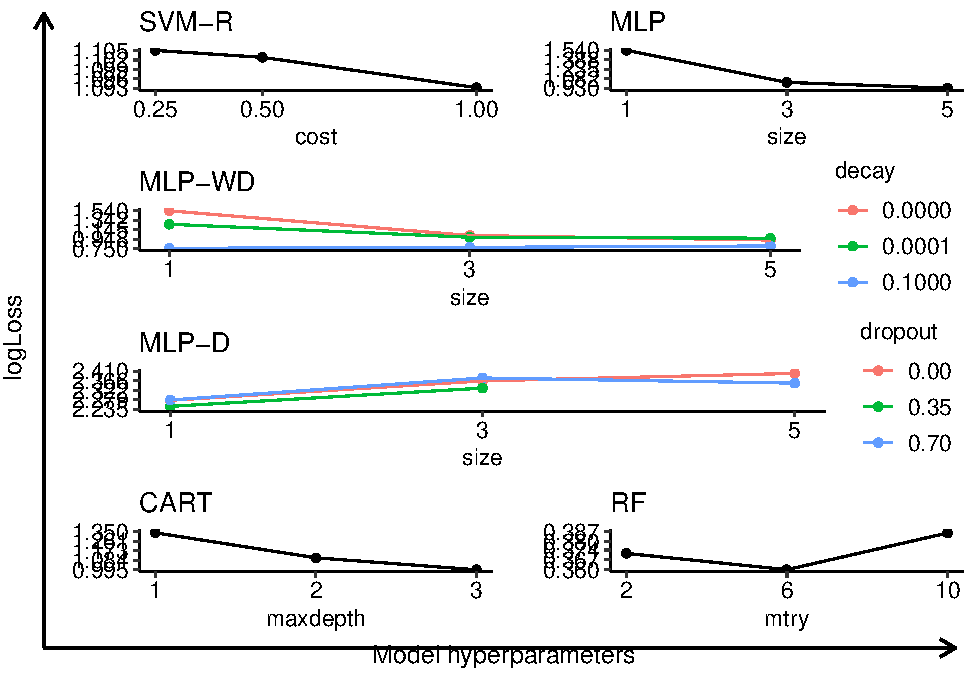
\includegraphics{sl-inf-cairs-2301_files/figure-latex/optResults2-2.pdf}

\begin{Shaded}
\begin{Highlighting}[]
\CommentTok{\#http://127.0.0.1:21067/graphics/plot\_zoom\_png?width=674\&height=678}
\FunctionTok{ggsave}\NormalTok{(}\AttributeTok{filename =} \StringTok{"results/plt\_hp\_5.jpeg"}\NormalTok{,}\AttributeTok{plot =} \FunctionTok{last\_plot}\NormalTok{(),}
       \AttributeTok{device =} \StringTok{"jpeg"}\NormalTok{,}\AttributeTok{height =} \DecValTok{678}\SpecialCharTok{/}\DecValTok{96}\NormalTok{,}\AttributeTok{width =} \DecValTok{674}\SpecialCharTok{/}\DecValTok{96}\NormalTok{,}\AttributeTok{dpi =} \DecValTok{600}\NormalTok{)}
\end{Highlighting}
\end{Shaded}

\hypertarget{validation-of-ml-models-on-test-data}{%
\section{Validation of ML models on test
data}\label{validation-of-ml-models-on-test-data}}

\begin{quote}
\hypertarget{getting-the-results-of-accuracy-kappa-and-logloss}{%
\subsubsection{Getting the results of Accuracy, Kappa and
logLoss}\label{getting-the-results-of-accuracy-kappa-and-logloss}}
\end{quote}

\begin{Shaded}
\begin{Highlighting}[]
\FunctionTok{set.seed}\NormalTok{(}\DecValTok{1226}\NormalTok{); test\_pred\_data}\OtherTok{\textless{}{-}}\FunctionTok{data.frame}\NormalTok{(}\AttributeTok{c=}\DecValTok{1}\SpecialCharTok{:}\DecValTok{1495}\NormalTok{)}
\FunctionTok{set.seed}\NormalTok{(}\DecValTok{1226}\NormalTok{)}
\NormalTok{Test\_result}\OtherTok{\textless{}{-}}\FunctionTok{data.frame}\NormalTok{(}\StringTok{"Accuracy"}\OtherTok{=}\DecValTok{1}\SpecialCharTok{:}\DecValTok{14}\NormalTok{, }\StringTok{"logLoss"}\OtherTok{=}\DecValTok{1}\SpecialCharTok{:}\DecValTok{14}\NormalTok{,}
                        \StringTok{"kappa"}\OtherTok{=}\DecValTok{1}\SpecialCharTok{:}\DecValTok{14}\NormalTok{,}\StringTok{"MCC"}\OtherTok{=}\DecValTok{1}\SpecialCharTok{:}\DecValTok{14}\NormalTok{,}
                        \AttributeTok{row.names=}\FunctionTok{names}\NormalTok{(Model\_list))}
\NormalTok{df\_test1}\OtherTok{\textless{}{-}}\FunctionTok{as\_tibble}\NormalTok{(df\_test)}
\CommentTok{\# Estimation of Accuracy of models  \#}
\FunctionTok{set.seed}\NormalTok{(}\DecValTok{1226}\NormalTok{)}
\NormalTok{Multi\_logloss }\OtherTok{\textless{}{-}} \ControlFlowTok{function}\NormalTok{(model, }\AttributeTok{df=}\NormalTok{df\_test1)\{}
  \FunctionTok{set.seed}\NormalTok{(}\DecValTok{1226}\NormalTok{)}
\NormalTok{  pred }\OtherTok{\textless{}{-}} \FunctionTok{predict}\NormalTok{(}\AttributeTok{object=}\NormalTok{model, df, }\AttributeTok{type =} \StringTok{\textquotesingle{}prob\textquotesingle{}}\NormalTok{,}\AttributeTok{verbose=}\NormalTok{F)}
\NormalTok{  logloss }\OtherTok{\textless{}{-}}\NormalTok{ MLmetrics}\SpecialCharTok{::}\FunctionTok{MultiLogLoss}\NormalTok{(}\AttributeTok{y\_true =}\NormalTok{ df}\SpecialCharTok{$}\NormalTok{Slump\_class,}
                                     \AttributeTok{y\_pred =} \FunctionTok{as.matrix}\NormalTok{(pred))}
  \FunctionTok{return}\NormalTok{(logloss)}
\NormalTok{\}}
\FunctionTok{set.seed}\NormalTok{(}\DecValTok{1226}\NormalTok{)}
\ControlFlowTok{for}\NormalTok{ (i }\ControlFlowTok{in} \FunctionTok{names}\NormalTok{(Model\_list)) \{}
  \FunctionTok{set.seed}\NormalTok{(}\DecValTok{1226}\NormalTok{)}
\NormalTok{  df\_test1[i] }\OtherTok{\textless{}{-}} \FunctionTok{predict}\NormalTok{(Model\_list[i],df\_test,}\AttributeTok{verbose=}\NormalTok{F)}
\NormalTok{  Test\_result[i,}\StringTok{"Accuracy"}\NormalTok{] }\OtherTok{\textless{}{-}} \FunctionTok{Accuracy}\NormalTok{(}\AttributeTok{y\_pred =} \FunctionTok{predict}\NormalTok{(Model\_list[[i]],}
                                                         \AttributeTok{newdata =}\NormalTok{ df\_test1),}
                                        \AttributeTok{y\_true =}\NormalTok{ df\_test}\SpecialCharTok{$}\NormalTok{Slump\_class)}

\NormalTok{  Test\_result[i,}\StringTok{"kappa"}\NormalTok{] }\OtherTok{\textless{}{-}} \FunctionTok{kappam.fleiss}\NormalTok{(}\FunctionTok{data.frame}\NormalTok{(df\_test1[,}\StringTok{"Slump\_class"}\NormalTok{],}
    \FunctionTok{predict}\NormalTok{(Model\_list[[i]], }\AttributeTok{newdata =}\NormalTok{ df\_test1)))}\SpecialCharTok{$}\NormalTok{value}
\NormalTok{  Test\_result[i,}\StringTok{"MCC"}\NormalTok{] }\OtherTok{\textless{}{-}} \FunctionTok{mcc}\NormalTok{(df\_test1}\SpecialCharTok{$}\NormalTok{Slump\_class,}
                              \FunctionTok{as.character}\NormalTok{(}\FunctionTok{predict}\NormalTok{(Model\_list[[i]],}
                                                   \AttributeTok{newdata =}\NormalTok{ df\_test1)))}
\NormalTok{  Test\_result[i,}\StringTok{"logLoss"}\NormalTok{] }\OtherTok{\textless{}{-}} \FunctionTok{Multi\_logloss}\NormalTok{(}\AttributeTok{model =}\NormalTok{ Model\_list[[i]],}
                                            \AttributeTok{df =}\NormalTok{ df\_test1)}
\NormalTok{\}}
\end{Highlighting}
\end{Shaded}

\begin{verbatim}
## Prediction uses 10 features.
## Prediction uses 10 features.
## Prediction uses 10 features.
## Prediction uses 10 features.
## Prediction uses 10 features.
\end{verbatim}

\begin{Shaded}
\begin{Highlighting}[]
\NormalTok{knitr}\SpecialCharTok{::}\FunctionTok{kable}\NormalTok{(Test\_result,}
             \AttributeTok{escape =}\NormalTok{ F,}
             \AttributeTok{col.names =} \FunctionTok{c}\NormalTok{(}\StringTok{"Accuracy"}\NormalTok{,}
                           \StringTok{"logLoss"}\NormalTok{,}\StringTok{"kappa"}\NormalTok{, }\StringTok{"MCC"}\NormalTok{),}
             \AttributeTok{digits =} \DecValTok{4}\NormalTok{,}
             \AttributeTok{format =} \StringTok{"simple"}\NormalTok{)}
\end{Highlighting}
\end{Shaded}

\begin{longtable}[]{@{}lrrrr@{}}
\toprule()
& Accuracy & logLoss & kappa & MCC \\
\midrule()
\endhead
RLR & 0.7070 & 0.7669 & 0.5727 & 0.5911 \\
GLM & 0.7191 & 0.7545 & 0.5892 & 0.6099 \\
LDA & 0.6615 & 1.0517 & 0.5232 & 0.5341 \\
SDA & 0.6615 & 1.0810 & 0.5232 & 0.5341 \\
SVM-L & 0.5532 & 1.1931 & 0.3135 & 0.3521 \\
SVM-P & 0.5953 & 1.1698 & 0.3835 & 0.4262 \\
SVM-R & 0.6140 & 1.0798 & 0.4167 & 0.4566 \\
MLP & 0.7472 & 0.9307 & 0.6419 & 0.6448 \\
MLP-WD & 0.4368 & 0.7619 & -0.2123 & 0.0000 \\
MLP-D & 0.2415 & 2.1836 & -0.1163 & -0.0187 \\
CART & 0.6361 & 0.9565 & 0.4794 & 0.5247 \\
C5.0 & 0.8682 & 0.4550 & 0.8188 & 0.8190 \\
RF & 0.8910 & 0.3374 & 0.8500 & 0.8511 \\
XGBoost & 0.8689 & 0.3553 & 0.8183 & 0.8196 \\
\bottomrule()
\end{longtable}

\begin{Shaded}
\begin{Highlighting}[]
\NormalTok{Test\_result}\SpecialCharTok{\%\textgreater{}\%}\FunctionTok{write.csv}\NormalTok{(}\StringTok{"results/test\_Results.csv"}\NormalTok{)}
\end{Highlighting}
\end{Shaded}

\begin{quote}
\hypertarget{defining-the-function-for-auc-for-roc-and-pr-curves}{%
\subsubsection{Defining the function for AUC for ROC and PR
curves}\label{defining-the-function-for-auc-for-roc-and-pr-curves}}
\end{quote}

\begin{Shaded}
\begin{Highlighting}[]
\NormalTok{df\_AUC\_curv}\OtherTok{\textless{}{-}}\NormalTok{df\_test1}
\ControlFlowTok{for}\NormalTok{ (i }\ControlFlowTok{in} \FunctionTok{names}\NormalTok{(df\_AUC\_curv[,}\DecValTok{20}\SpecialCharTok{:}\FunctionTok{length}\NormalTok{(df\_test1)])) \{}
\NormalTok{  df\_AUC\_curv[,i]}\OtherTok{\textless{}{-}}\FunctionTok{gsub}\NormalTok{(}\AttributeTok{pattern =} \StringTok{"sl\_"}\NormalTok{,}\AttributeTok{replacement =} \StringTok{""}\NormalTok{,}
                        \AttributeTok{x =} \FunctionTok{unlist}\NormalTok{(df\_AUC\_curv[,i]))}
\NormalTok{  df\_AUC\_curv[,i]}\OtherTok{\textless{}{-}}\FunctionTok{factor}\NormalTok{(}\AttributeTok{x =} \FunctionTok{unlist}\NormalTok{(df\_AUC\_curv[,i]),}
                          \AttributeTok{levels =} \FunctionTok{c}\NormalTok{(}\StringTok{"25mm"}\NormalTok{,}\StringTok{"75mm"}\NormalTok{, }\StringTok{"80mm"}\NormalTok{,}\StringTok{"100mm"}\NormalTok{,}
                                     \StringTok{"125mm"}\NormalTok{,}\StringTok{"135mm"}\NormalTok{,}\StringTok{"150mm"}\NormalTok{,}
                                     \StringTok{"175mm"}\NormalTok{,}\StringTok{"200mm"}\NormalTok{))}
\NormalTok{  \}}

\NormalTok{AUC}\OtherTok{\textless{}{-}}\ControlFlowTok{function}\NormalTok{(}\AttributeTok{model=}\NormalTok{fit\_01regLogistic,}\AttributeTok{df=}\NormalTok{df\_AUC\_curv, }\AttributeTok{ggtitle=}\FunctionTok{ggtitle}\NormalTok{(}\StringTok{"RLR"}\NormalTok{),}
              \AttributeTok{method=}\StringTok{"\_pred\_fit\_rlr"}\NormalTok{, }\AttributeTok{un=}\FunctionTok{c}\NormalTok{(}\FloatTok{0.0}\NormalTok{,}\FloatTok{0.2}\NormalTok{,}\DecValTok{0}\NormalTok{,}\DecValTok{0}\NormalTok{),}
              \AttributeTok{x.text=}\FunctionTok{element\_text}\NormalTok{()) \{}
\NormalTok{    x.text}\OtherTok{=}\NormalTok{x.text}
\NormalTok{    un}\OtherTok{=}\NormalTok{un}
\NormalTok{    levels }\OtherTok{=} \FunctionTok{c}\NormalTok{(}\StringTok{"25mm"}\NormalTok{,}\StringTok{"75mm"}\NormalTok{, }\StringTok{"80mm"}\NormalTok{,}\StringTok{"100mm"}\NormalTok{,}\StringTok{"125mm"}\NormalTok{,}\StringTok{"135mm"}\NormalTok{,}\StringTok{"150mm"}\NormalTok{,}
               \StringTok{"175mm"}\NormalTok{,}\StringTok{"200mm"}\NormalTok{,}\StringTok{"Macro"}\NormalTok{,}\StringTok{"Micro"}\NormalTok{)}
\NormalTok{    colorLevels }\OtherTok{=} \FunctionTok{c}\NormalTok{(}\StringTok{"\#EEDFCC"}\NormalTok{,}\StringTok{"\#66CDAA"}\NormalTok{,}\StringTok{"\#C1CDCD"}\NormalTok{,}\StringTok{"\#0000CD"}\NormalTok{,}\StringTok{"\#000000"}\NormalTok{,}
                    \StringTok{"\#CD3333"}\NormalTok{,}\StringTok{"\#FFFF00"}\NormalTok{,}\StringTok{"\#66CD00"}\NormalTok{,}\StringTok{"\#FF7F00"}\NormalTok{,}\StringTok{"\#008B00"}\NormalTok{,}\StringTok{"\#003B00"}\NormalTok{)}
    \FunctionTok{set.seed}\NormalTok{(}\DecValTok{1226}\NormalTok{)}
\NormalTok{    pred }\OtherTok{=} \FunctionTok{data.frame}\NormalTok{(}\FunctionTok{predict}\NormalTok{(model, df, }\AttributeTok{type =} \StringTok{\textquotesingle{}prob\textquotesingle{}}\NormalTok{))}
    \FunctionTok{colnames}\NormalTok{(pred)}\OtherTok{=}\FunctionTok{paste}\NormalTok{(}\FunctionTok{gsub}\NormalTok{(}\StringTok{"sl\_"}\NormalTok{, }\StringTok{""}\NormalTok{, }\FunctionTok{colnames}\NormalTok{(pred)))}
    \FunctionTok{colnames}\NormalTok{(pred)}\OtherTok{=}\FunctionTok{paste}\NormalTok{(}\FunctionTok{colnames}\NormalTok{(pred), method,}\AttributeTok{sep =} \StringTok{""}\NormalTok{)}
\NormalTok{    true\_label }\OtherTok{=} \FunctionTok{data.frame}\NormalTok{(dummy}\SpecialCharTok{::}\FunctionTok{dummy}\NormalTok{(df\_AUC\_curv[}\StringTok{\textquotesingle{}Slump\_class\textquotesingle{}}\NormalTok{]))}
\NormalTok{    cnames}\OtherTok{=}\NormalTok{levels[}\DecValTok{1}\SpecialCharTok{:}\DecValTok{9}\NormalTok{]}
    \FunctionTok{colnames}\NormalTok{(true\_label) }\OtherTok{=}\NormalTok{ cnames}
    \FunctionTok{colnames}\NormalTok{(true\_label) }\OtherTok{=} \FunctionTok{paste}\NormalTok{(}\FunctionTok{colnames}\NormalTok{(true\_label), }\StringTok{"\_true"}\NormalTok{,}\AttributeTok{sep =} \StringTok{""}\NormalTok{)}
    \FunctionTok{set.seed}\NormalTok{(}\DecValTok{1226}\NormalTok{)}
\NormalTok{    AUC\_df }\OtherTok{=} \FunctionTok{cbind}\NormalTok{(true\_label, pred)}
    \FunctionTok{set.seed}\NormalTok{(}\DecValTok{1226}\NormalTok{)}
    \CommentTok{\# ROC Estimation}
\NormalTok{    AUC\_SS }\OtherTok{=} \FunctionTok{multi\_roc}\NormalTok{(AUC\_df)}
\NormalTok{    Plot\_AUC\_SS }\OtherTok{=} \FunctionTok{plot\_roc\_data}\NormalTok{(AUC\_SS)}
\NormalTok{    Plot\_AUC\_SS}\SpecialCharTok{$}\NormalTok{Group}\SpecialCharTok{\%\textgreater{}\%}\FunctionTok{unique}\NormalTok{()}
\NormalTok{    Plot\_AUC\_SS}\SpecialCharTok{$}\NormalTok{Group }\OtherTok{=} \FunctionTok{factor}\NormalTok{(Plot\_AUC\_SS}\SpecialCharTok{$}\NormalTok{Group,}\AttributeTok{levels =}\NormalTok{ levels)}
\NormalTok{    Plot\_AUC\_SS}\SpecialCharTok{$}\NormalTok{gmean}\OtherTok{=}\FunctionTok{sqrt}\NormalTok{(Plot\_AUC\_SS}\SpecialCharTok{$}\NormalTok{Sensitivity}\SpecialCharTok{*}\NormalTok{Plot\_AUC\_SS}\SpecialCharTok{$}\NormalTok{Specificity)}
\NormalTok{    ss}\OtherTok{\textless{}{-}} \FunctionTok{ggplot}\NormalTok{(Plot\_AUC\_SS, }\FunctionTok{aes}\NormalTok{(}\AttributeTok{x =} \DecValTok{1}\SpecialCharTok{{-}}\NormalTok{Specificity, }\AttributeTok{y=}\NormalTok{Sensitivity)) }\SpecialCharTok{+}
      \FunctionTok{geom\_path}\NormalTok{(}\FunctionTok{aes}\NormalTok{(}\AttributeTok{color =}\NormalTok{ Group), }\AttributeTok{size=}\FloatTok{0.50}\NormalTok{) }\SpecialCharTok{+}
      \FunctionTok{geom\_segment}\NormalTok{(}\FunctionTok{aes}\NormalTok{(}\AttributeTok{x =} \DecValTok{0}\NormalTok{, }\AttributeTok{y =} \DecValTok{0}\NormalTok{, }\AttributeTok{xend =} \DecValTok{1}\NormalTok{, }\AttributeTok{yend =} \DecValTok{1}\NormalTok{),}
                   \AttributeTok{colour=}\StringTok{\textquotesingle{}grey\textquotesingle{}}\NormalTok{, }\AttributeTok{linetype =} \StringTok{\textquotesingle{}dotdash\textquotesingle{}}\NormalTok{) }\SpecialCharTok{+}
\NormalTok{      ggtitle }\SpecialCharTok{+} \FunctionTok{theme\_classic}\NormalTok{() }\SpecialCharTok{+} \FunctionTok{labs}\NormalTok{ (}\AttributeTok{x=}\StringTok{""}\NormalTok{,}\AttributeTok{y=}\StringTok{""}\NormalTok{) }\SpecialCharTok{+}
      \FunctionTok{theme}\NormalTok{(}
        \CommentTok{\# axis.title = element\_text(face = "bold"),}
        \AttributeTok{axis.text =} \FunctionTok{element\_text}\NormalTok{(}\AttributeTok{size =} \DecValTok{12}\NormalTok{,}\AttributeTok{color =} \StringTok{"black"}\NormalTok{),}
        \CommentTok{\# axis.text.x = x.text,}
        \AttributeTok{plot.title =} \FunctionTok{element\_text}\NormalTok{(}\AttributeTok{size =} \DecValTok{12}\NormalTok{,}\AttributeTok{face =} \StringTok{"plain"}\NormalTok{,}
                                      \AttributeTok{colour =} \StringTok{"\#04456b"}\NormalTok{),}
        \AttributeTok{plot.margin =} \FunctionTok{unit}\NormalTok{(un,}\StringTok{"cm"}\NormalTok{),}
        \AttributeTok{legend.title =} \FunctionTok{element\_blank}\NormalTok{(),}
        \AttributeTok{legend.position=}\StringTok{"bottom"}\NormalTok{,}\AttributeTok{legend.direction =} \StringTok{"horizontal"}\NormalTok{,}
        \AttributeTok{legend.background =} \FunctionTok{element\_rect}\NormalTok{(}\AttributeTok{fill=}\ConstantTok{NULL}\NormalTok{, }\AttributeTok{size=}\FloatTok{0.5}\NormalTok{,}
                                         \AttributeTok{linetype=}\StringTok{"dotted"}\NormalTok{,}\AttributeTok{colour =}\StringTok{"black"}\NormalTok{)) }\SpecialCharTok{+}
      \FunctionTok{scale\_colour\_manual}\NormalTok{(}\AttributeTok{values =}\NormalTok{ colorLevels)}
\NormalTok{    legend\_ROC}\OtherTok{\textless{}{-}} \FunctionTok{get\_legend}\NormalTok{(ss)}
\NormalTok{    ss }\OtherTok{\textless{}{-}}\NormalTok{ ss}\SpecialCharTok{+}\FunctionTok{theme}\NormalTok{(}\AttributeTok{legend.position =} \StringTok{"none"}\NormalTok{)}
  
    \CommentTok{\# PR estimation}
    \FunctionTok{set.seed}\NormalTok{(}\DecValTok{1226}\NormalTok{)}
\NormalTok{    AUC\_PR }\OtherTok{=} \FunctionTok{multi\_pr}\NormalTok{(AUC\_df)}
\NormalTok{    Plot\_AUC\_PR }\OtherTok{=} \FunctionTok{plot\_pr\_data}\NormalTok{(AUC\_PR)}
\NormalTok{    Plot\_AUC\_PR}\SpecialCharTok{$}\NormalTok{Group }\OtherTok{=} \FunctionTok{factor}\NormalTok{(Plot\_AUC\_PR}\SpecialCharTok{$}\NormalTok{Group,}\AttributeTok{levels =}\NormalTok{ levels)}
\NormalTok{    Plot\_AUC\_PR}\SpecialCharTok{$}\NormalTok{fscore }\OtherTok{=}\NormalTok{ (}\DecValTok{2}\SpecialCharTok{*}\NormalTok{Plot\_AUC\_PR}\SpecialCharTok{$}\NormalTok{Precision}\SpecialCharTok{*}\NormalTok{Plot\_AUC\_PR}\SpecialCharTok{$}\NormalTok{Recall)}\SpecialCharTok{/}
\NormalTok{      (Plot\_AUC\_PR}\SpecialCharTok{$}\NormalTok{Precision }\SpecialCharTok{+}\NormalTok{ Plot\_AUC\_PR}\SpecialCharTok{$}\NormalTok{Recall)}
\NormalTok{    pr}\OtherTok{\textless{}{-}} \FunctionTok{ggplot}\NormalTok{(Plot\_AUC\_PR, }\FunctionTok{aes}\NormalTok{(}\AttributeTok{x=}\NormalTok{Recall, }\AttributeTok{y=}\NormalTok{Precision)) }\SpecialCharTok{+}
      \FunctionTok{geom\_path}\NormalTok{(}\FunctionTok{aes}\NormalTok{(}\AttributeTok{color =}\NormalTok{ Group), }\AttributeTok{size=}\FloatTok{0.5}\NormalTok{) }\SpecialCharTok{+}
      \FunctionTok{geom\_segment}\NormalTok{(}\FunctionTok{aes}\NormalTok{(}\AttributeTok{x =} \DecValTok{0}\NormalTok{, }\AttributeTok{y =} \DecValTok{1}\NormalTok{, }\AttributeTok{xend =} \DecValTok{1}\NormalTok{, }\AttributeTok{yend =} \DecValTok{0}\NormalTok{),}
                   \AttributeTok{colour=}\StringTok{\textquotesingle{}grey\textquotesingle{}}\NormalTok{, }\AttributeTok{linetype =} \StringTok{\textquotesingle{}dotdash\textquotesingle{}}\NormalTok{) }\SpecialCharTok{+}
\NormalTok{      ggtitle }\SpecialCharTok{+} \FunctionTok{theme\_classic}\NormalTok{() }\SpecialCharTok{+} \FunctionTok{labs}\NormalTok{ (}\AttributeTok{x=}\StringTok{""}\NormalTok{,}\AttributeTok{y=}\StringTok{""}\NormalTok{) }\SpecialCharTok{+}
      \FunctionTok{theme}\NormalTok{(}
        \CommentTok{\# axis.text.x = x.text,}
        \AttributeTok{axis.text =} \FunctionTok{element\_text}\NormalTok{(}\AttributeTok{size =} \DecValTok{12}\NormalTok{,}\AttributeTok{color =} \StringTok{"black"}\NormalTok{),}
        \AttributeTok{plot.title =} \FunctionTok{element\_text}\NormalTok{(}\AttributeTok{size =} \DecValTok{12}\NormalTok{,}\AttributeTok{face =} \StringTok{"plain"}\NormalTok{,}\AttributeTok{colour =} \StringTok{"\#04456b"}\NormalTok{),}
        \AttributeTok{plot.margin =} \FunctionTok{unit}\NormalTok{(un,}\StringTok{"cm"}\NormalTok{),}
        \AttributeTok{legend.title=}\FunctionTok{element\_blank}\NormalTok{(),}
        \AttributeTok{legend.position=}\StringTok{"bottom"}\NormalTok{,}\AttributeTok{legend.direction =} \StringTok{"horizontal"}\NormalTok{,}
\NormalTok{        legend.background}
        \OtherTok{=} \FunctionTok{element\_rect}\NormalTok{(}\AttributeTok{fill=}\ConstantTok{NULL}\NormalTok{, }\AttributeTok{size=}\FloatTok{0.5}\NormalTok{,}
                                         \AttributeTok{linetype=}\StringTok{"dotted"}\NormalTok{, }\AttributeTok{colour =}\StringTok{"black"}\NormalTok{))}\SpecialCharTok{+}
    \CommentTok{\# scale\_colour\_manual(values = rainbow(10))+}
    \FunctionTok{scale\_colour\_manual}\NormalTok{(}\AttributeTok{values =}\NormalTok{  colorLevels)}
\NormalTok{    legend\_pr}\OtherTok{\textless{}{-}} \FunctionTok{get\_legend}\NormalTok{(pr)}
\NormalTok{    pr }\OtherTok{\textless{}{-}}\NormalTok{ pr}\SpecialCharTok{+}\FunctionTok{theme}\NormalTok{(}\AttributeTok{legend.position =} \StringTok{"none"}\NormalTok{)}
    \FunctionTok{return}\NormalTok{(}\FunctionTok{list}\NormalTok{(}\StringTok{"ss"}\OtherTok{=}\NormalTok{ss,}\StringTok{"pr"}\OtherTok{=}\NormalTok{pr,}\StringTok{"ROC"}\OtherTok{=}\NormalTok{AUC\_SS,}\StringTok{"PR"}\OtherTok{=}\NormalTok{AUC\_PR,}\StringTok{"df\_roc"}\OtherTok{=}\NormalTok{Plot\_AUC\_SS,}
                \StringTok{"df\_pr"}\OtherTok{=}\NormalTok{Plot\_AUC\_PR,}\StringTok{"leg\_ss"}\OtherTok{=}\NormalTok{legend\_ROC,}\StringTok{"leg\_pr"}\OtherTok{=}\NormalTok{legend\_pr))}
\NormalTok{\}}
\end{Highlighting}
\end{Shaded}

\begin{quote}
\hypertarget{getting-and-drawing-the-results-of-auc}{%
\subsubsection{Getting and Drawing the results of
AUC}\label{getting-and-drawing-the-results-of-auc}}
\end{quote}

\begin{Shaded}
\begin{Highlighting}[]
\FunctionTok{set.seed}\NormalTok{(}\DecValTok{1226}\NormalTok{)}
\NormalTok{AUC\_rlr }\OtherTok{\textless{}{-}} \FunctionTok{AUC}\NormalTok{(}\AttributeTok{model=}\NormalTok{ fit\_01regLogistic, }\AttributeTok{ggtitle=} \FunctionTok{ggtitle}\NormalTok{(}\StringTok{"RLR"}\NormalTok{),}
               \AttributeTok{method =} \StringTok{"\_pred\_fit\_01regLogistic"}\NormalTok{,}
               \AttributeTok{un=} \FunctionTok{c}\NormalTok{(}\FloatTok{0.2}\NormalTok{,}\FloatTok{0.2}\NormalTok{,}\FloatTok{0.0}\NormalTok{,}\DecValTok{0}\NormalTok{))}
\NormalTok{AUC\_glm }\OtherTok{\textless{}{-}} \FunctionTok{AUC}\NormalTok{(}\AttributeTok{model=}\NormalTok{ fit\_02glmnet,}\AttributeTok{ggtitle=} \FunctionTok{ggtitle}\NormalTok{(}\StringTok{"GLM"}\NormalTok{),}
               \AttributeTok{method =} \StringTok{"\_pred\_fit\_02glmnet"}\NormalTok{,}
               \AttributeTok{un=} \FunctionTok{c}\NormalTok{(}\FloatTok{0.2}\NormalTok{,}\FloatTok{0.2}\NormalTok{,}\FloatTok{0.0}\NormalTok{,}\DecValTok{0}\NormalTok{))}
\NormalTok{AUC\_lda }\OtherTok{\textless{}{-}} \FunctionTok{AUC}\NormalTok{(}\AttributeTok{model=}\NormalTok{ fit\_03lda, }\AttributeTok{ggtitle=} \FunctionTok{ggtitle}\NormalTok{(}\StringTok{"LDA"}\NormalTok{),}
               \AttributeTok{method =} \StringTok{"\_pred\_fit\_03lda"}\NormalTok{,}
               \AttributeTok{un=} \FunctionTok{c}\NormalTok{(}\FloatTok{0.2}\NormalTok{,}\FloatTok{0.2}\NormalTok{,}\FloatTok{0.0}\NormalTok{,}\DecValTok{0}\NormalTok{))}
\NormalTok{AUC\_sda }\OtherTok{\textless{}{-}} \FunctionTok{AUC}\NormalTok{(}\AttributeTok{model=}\NormalTok{ fit\_04sda, }\AttributeTok{ggtitle=} \FunctionTok{ggtitle}\NormalTok{(}\StringTok{"SDA"}\NormalTok{),}
               \AttributeTok{method=} \StringTok{"\_pred\_fit\_04sda"}\NormalTok{,}
               \AttributeTok{un=} \FunctionTok{c}\NormalTok{(}\FloatTok{0.2}\NormalTok{,}\FloatTok{0.2}\NormalTok{,}\FloatTok{0.0}\NormalTok{,}\DecValTok{0}\NormalTok{))}
\end{Highlighting}
\end{Shaded}

\begin{verbatim}
## Prediction uses 10 features.
\end{verbatim}

\begin{Shaded}
\begin{Highlighting}[]
\NormalTok{AUC\_mlp }\OtherTok{\textless{}{-}} \FunctionTok{AUC}\NormalTok{(}\AttributeTok{model=}\NormalTok{ fit\_05mlp, }\AttributeTok{ggtitle=} \FunctionTok{ggtitle}\NormalTok{(}\StringTok{"MLP"}\NormalTok{),}
                \AttributeTok{method=} \StringTok{"\_pred\_fit\_05mlp"}\NormalTok{,}
               \AttributeTok{un=} \FunctionTok{c}\NormalTok{(}\FloatTok{0.0}\NormalTok{,}\FloatTok{0.2}\NormalTok{,}\FloatTok{0.0}\NormalTok{,}\DecValTok{0}\NormalTok{))}
\NormalTok{AUC\_mlpD }\OtherTok{\textless{}{-}} \FunctionTok{AUC}\NormalTok{(}\AttributeTok{model=}\NormalTok{ fit\_06mlpWD, }\AttributeTok{ggtitle=} \FunctionTok{ggtitle}\NormalTok{(}\StringTok{"MLP{-}WD"}\NormalTok{),}
              \AttributeTok{method =} \StringTok{"\_pred\_fit\_06mlpWD"}\NormalTok{,}
               \AttributeTok{un=} \FunctionTok{c}\NormalTok{(}\FloatTok{0.0}\NormalTok{,}\FloatTok{0.2}\NormalTok{,}\FloatTok{0.0}\NormalTok{,}\DecValTok{0}\NormalTok{))}
\NormalTok{AUC\_mlpWD }\OtherTok{\textless{}{-}} \FunctionTok{AUC}\NormalTok{(}\AttributeTok{model=}\NormalTok{ fit\_07mlpKerasDropout,}\AttributeTok{ggtitle=} \FunctionTok{ggtitle}\NormalTok{(}\StringTok{"MLP{-}D"}\NormalTok{),}
               \AttributeTok{method =} \StringTok{"\_pred\_fit\_07mlpKerasDropout"}\NormalTok{,}
               \AttributeTok{un=} \FunctionTok{c}\NormalTok{(}\FloatTok{0.0}\NormalTok{,}\FloatTok{0.2}\NormalTok{,}\FloatTok{0.0}\NormalTok{,}\DecValTok{0}\NormalTok{))}
\NormalTok{AUC\_svml }\OtherTok{\textless{}{-}} \FunctionTok{AUC}\NormalTok{(}\AttributeTok{model=}\NormalTok{ fit\_08svml,}\AttributeTok{ggtitle=} \FunctionTok{ggtitle}\NormalTok{(}\StringTok{"SVM{-}L"}\NormalTok{),}
                \AttributeTok{method=} \StringTok{"\_pred\_fit\_08svml"}\NormalTok{,}
               \AttributeTok{un=} \FunctionTok{c}\NormalTok{(}\FloatTok{0.0}\NormalTok{,}\FloatTok{0.2}\NormalTok{,}\FloatTok{0.0}\NormalTok{,}\DecValTok{0}\NormalTok{))}
\NormalTok{AUC\_svmp }\OtherTok{\textless{}{-}} \FunctionTok{AUC}\NormalTok{(}\AttributeTok{model=}\NormalTok{ fit\_09svmp,}\AttributeTok{ggtitle=} \FunctionTok{ggtitle}\NormalTok{(}\StringTok{"SVM{-}P"}\NormalTok{),}
              \AttributeTok{method =} \StringTok{"\_pred\_fit\_09svmp"}\NormalTok{,}
               \AttributeTok{un=} \FunctionTok{c}\NormalTok{(}\FloatTok{0.0}\NormalTok{,}\FloatTok{0.2}\NormalTok{,}\FloatTok{0.0}\NormalTok{,}\DecValTok{0}\NormalTok{))}
\NormalTok{AUC\_svmR }\OtherTok{\textless{}{-}} \FunctionTok{AUC}\NormalTok{(}\AttributeTok{model=}\NormalTok{ fit\_10svmr,}\AttributeTok{ggtitle=} \FunctionTok{ggtitle}\NormalTok{(}\StringTok{"SVM{-}R"}\NormalTok{),}
               \AttributeTok{method =} \StringTok{"\_pred\_fit\_10svmr"}\NormalTok{,}
               \AttributeTok{un=} \FunctionTok{c}\NormalTok{(}\FloatTok{0.0}\NormalTok{,}\FloatTok{0.2}\NormalTok{,}\FloatTok{0.0}\NormalTok{,}\DecValTok{0}\NormalTok{),}
               \AttributeTok{x.text =} \FunctionTok{element\_text}\NormalTok{())}
\NormalTok{AUC\_CART }\OtherTok{\textless{}{-}} \FunctionTok{AUC}\NormalTok{(}\AttributeTok{model=}\NormalTok{ fit\_11cart,}\AttributeTok{ggtitle=} \FunctionTok{ggtitle}\NormalTok{(}\StringTok{"CART"}\NormalTok{),}
               \AttributeTok{method =} \StringTok{"\_pred\_fit\_11cart"}\NormalTok{,}
               \AttributeTok{un=} \FunctionTok{c}\NormalTok{(}\FloatTok{0.0}\NormalTok{,}\FloatTok{0.2}\NormalTok{,}\FloatTok{0.0}\NormalTok{,}\DecValTok{0}\NormalTok{),}
               \AttributeTok{x.text =} \FunctionTok{element\_text}\NormalTok{())}
\NormalTok{AUC\_C5 }\OtherTok{\textless{}{-}} \FunctionTok{AUC}\NormalTok{(}\AttributeTok{model=}\NormalTok{ fit\_12C5,}\AttributeTok{ggtitle=} \FunctionTok{ggtitle}\NormalTok{(}\StringTok{"C5.0"}\NormalTok{),}
                \AttributeTok{method=} \StringTok{"\_pred\_fit\_12C5"}\NormalTok{,}
               \AttributeTok{un=} \FunctionTok{c}\NormalTok{(}\FloatTok{0.0}\NormalTok{,}\FloatTok{0.2}\NormalTok{,}\FloatTok{0.0}\NormalTok{,}\DecValTok{0}\NormalTok{),}
               \AttributeTok{x.text =} \FunctionTok{element\_text}\NormalTok{())}
\NormalTok{AUC\_RF }\OtherTok{\textless{}{-}} \FunctionTok{AUC}\NormalTok{(}\AttributeTok{model=}\NormalTok{ fit\_13rf,}\AttributeTok{ggtitle=} \FunctionTok{ggtitle}\NormalTok{(}\StringTok{"RF"}\NormalTok{),}
              \AttributeTok{method =} \StringTok{"\_pred\_fit\_13rf"}\NormalTok{,}
               \AttributeTok{un=} \FunctionTok{c}\NormalTok{(}\FloatTok{0.0}\NormalTok{,}\FloatTok{0.2}\NormalTok{,}\FloatTok{0.0}\NormalTok{,}\DecValTok{0}\NormalTok{),}
               \AttributeTok{x.text =} \FunctionTok{element\_text}\NormalTok{())}
\NormalTok{AUC\_xgb }\OtherTok{\textless{}{-}} \FunctionTok{AUC}\NormalTok{(}\AttributeTok{model=}\NormalTok{ fit\_14xgb,}\AttributeTok{ggtitle=} \FunctionTok{ggtitle}\NormalTok{(}\StringTok{"XGBoost"}\NormalTok{),}
               \AttributeTok{method =} \StringTok{"\_pred\_fit\_14xgb"}\NormalTok{,}
               \AttributeTok{un=} \FunctionTok{c}\NormalTok{(}\FloatTok{0.0}\NormalTok{,}\FloatTok{0.2}\NormalTok{,}\FloatTok{0.0}\NormalTok{,}\DecValTok{0}\NormalTok{),}
               \AttributeTok{x.text =} \FunctionTok{element\_text}\NormalTok{())}
\end{Highlighting}
\end{Shaded}

\begin{quote}
\hypertarget{roc-plot}{%
\subsubsection{ROC Plot}\label{roc-plot}}
\end{quote}

\begin{Shaded}
\begin{Highlighting}[]
\NormalTok{plt\_layout\_matrix }\OtherTok{=} \FunctionTok{rbind}\NormalTok{(}\FunctionTok{c}\NormalTok{(}\DecValTok{1}\SpecialCharTok{:}\DecValTok{4}\NormalTok{),}\FunctionTok{c}\NormalTok{(}\DecValTok{5}\SpecialCharTok{:}\DecValTok{8}\NormalTok{),}\FunctionTok{c}\NormalTok{(}\DecValTok{9}\SpecialCharTok{:}\DecValTok{12}\NormalTok{),}\FunctionTok{c}\NormalTok{(}\DecValTok{13}\NormalTok{,}\DecValTok{14}\NormalTok{,}\DecValTok{15}\NormalTok{,}\DecValTok{15}\NormalTok{))}
\NormalTok{auc\_roc\_all}\OtherTok{\textless{}{-}}\FunctionTok{arrangeGrob}\NormalTok{(}
  \AttributeTok{grobs=} \FunctionTok{list}\NormalTok{(AUC\_rlr}\SpecialCharTok{$}\NormalTok{ss,AUC\_glm}\SpecialCharTok{$}\NormalTok{ss,AUC\_lda}\SpecialCharTok{$}\NormalTok{ss,AUC\_sda}\SpecialCharTok{$}\NormalTok{ss,AUC\_mlp}\SpecialCharTok{$}\NormalTok{ss,}
\NormalTok{              AUC\_mlpD}\SpecialCharTok{$}\NormalTok{ss,AUC\_mlpWD}\SpecialCharTok{$}\NormalTok{ss,AUC\_svml}\SpecialCharTok{$}\NormalTok{ss,AUC\_svmp}\SpecialCharTok{$}\NormalTok{ss,AUC\_svmR}\SpecialCharTok{$}\NormalTok{ss,}
\NormalTok{              AUC\_CART}\SpecialCharTok{$}\NormalTok{ss,AUC\_C5}\SpecialCharTok{$}\NormalTok{ss,AUC\_RF}\SpecialCharTok{$}\NormalTok{ss,AUC\_xgb}\SpecialCharTok{$}\NormalTok{ss,AUC\_rlr}\SpecialCharTok{$}\NormalTok{leg\_ss),}
  \AttributeTok{nrow =}\DecValTok{4}\NormalTok{,}\AttributeTok{ncol =} \DecValTok{4}\NormalTok{,}\AttributeTok{layout\_matrix =}\NormalTok{ plt\_layout\_matrix)}

\NormalTok{auc\_roc\_all}\OtherTok{\textless{}{-}} \FunctionTok{annotate\_figure}\NormalTok{(}
  \AttributeTok{p =}\NormalTok{ auc\_roc\_all,}
  \AttributeTok{left =} \FunctionTok{text\_grob}\NormalTok{(}\StringTok{"Sensitivity"}\NormalTok{,}\AttributeTok{face =} \StringTok{"plain"}\NormalTok{,}
                   \AttributeTok{rot =} \DecValTok{90}\NormalTok{, }\AttributeTok{size =} \DecValTok{12}\NormalTok{,}\AttributeTok{vjust =} \FloatTok{1.0}\NormalTok{),}
  \AttributeTok{bottom =} \FunctionTok{text\_grob}\NormalTok{(}\StringTok{"1{-}Specificity"}\NormalTok{, }\AttributeTok{face =} \StringTok{"plain"}\NormalTok{,}
                     \AttributeTok{size =} \DecValTok{12}\NormalTok{,}\AttributeTok{vjust =} \FloatTok{0.05}\NormalTok{))}

\NormalTok{auc\_roc\_all}\OtherTok{\textless{}{-}}\NormalTok{ auc\_roc\_all }\SpecialCharTok{+}
  \FunctionTok{geom\_segment}\NormalTok{(}\FunctionTok{aes}\NormalTok{(}\AttributeTok{x =}\NormalTok{ .}\DecValTok{030}\NormalTok{, }\AttributeTok{y=}\FloatTok{0.02}\NormalTok{, }\AttributeTok{xend=}\FloatTok{0.030}\NormalTok{, }\AttributeTok{yend =}\NormalTok{ .}\DecValTok{98}\NormalTok{), }\AttributeTok{size =}\NormalTok{.}\DecValTok{6}\NormalTok{,}
               \AttributeTok{arrow =} \FunctionTok{arrow}\NormalTok{(}\AttributeTok{length =} \FunctionTok{unit}\NormalTok{(}\FloatTok{0.3}\NormalTok{, }\StringTok{"cm"}\NormalTok{))) }\SpecialCharTok{+}
  \FunctionTok{geom\_segment}\NormalTok{(}\FunctionTok{aes}\NormalTok{(}\AttributeTok{x =}\NormalTok{ .}\DecValTok{030}\NormalTok{, }\AttributeTok{y=}\FloatTok{0.02}\NormalTok{, }\AttributeTok{xend=}\FloatTok{0.98}\NormalTok{, }\AttributeTok{yend =}\NormalTok{ .}\DecValTok{02}\NormalTok{), }\AttributeTok{size =}\NormalTok{.}\DecValTok{6}\NormalTok{,}
               \AttributeTok{arrow =} \FunctionTok{arrow}\NormalTok{(}\AttributeTok{length =} \FunctionTok{unit}\NormalTok{(}\FloatTok{0.3}\NormalTok{, }\StringTok{"cm"}\NormalTok{)))}

\NormalTok{auc\_roc\_all}
\end{Highlighting}
\end{Shaded}

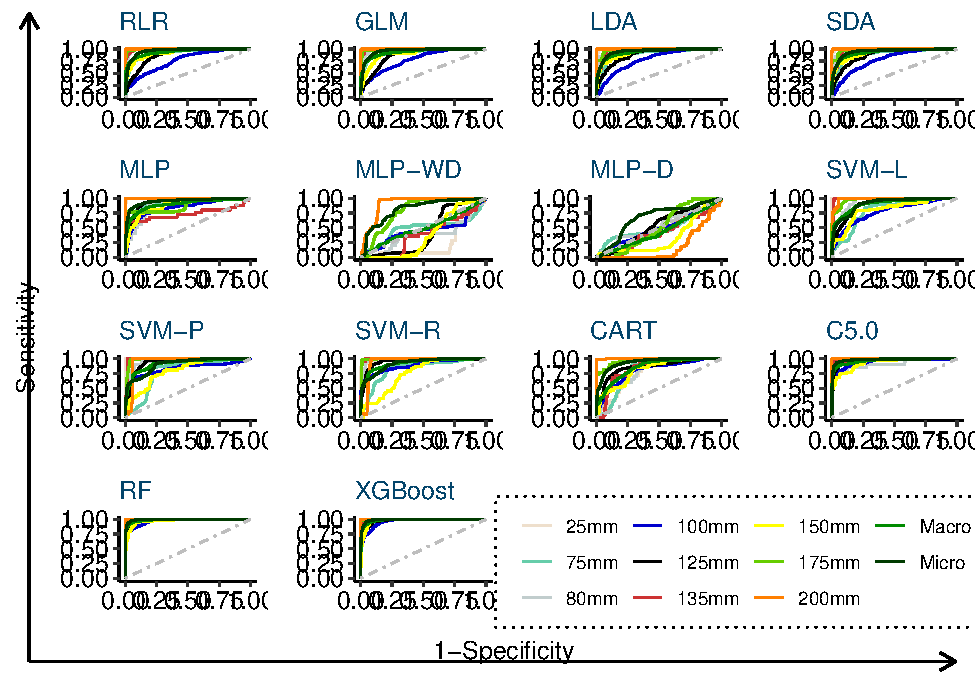
\includegraphics{sl-inf-cairs-2301_files/figure-latex/AUCplots-1.pdf}

\begin{Shaded}
\begin{Highlighting}[]
\FunctionTok{ggsave}\NormalTok{(}\AttributeTok{filename =} \StringTok{"results/plt\_AUCROC\_all4.jpeg"}\NormalTok{,}\AttributeTok{plot =} \FunctionTok{last\_plot}\NormalTok{(),}
\AttributeTok{device =} \StringTok{"jpeg"}\NormalTok{,}\AttributeTok{width =} \DecValTok{1109}\SpecialCharTok{/}\DecValTok{96}\NormalTok{,}\AttributeTok{height =} \DecValTok{1482}\SpecialCharTok{/}\DecValTok{96}\NormalTok{,}\AttributeTok{dpi =} \DecValTok{600}\NormalTok{)}
\end{Highlighting}
\end{Shaded}

\begin{quote}
\hypertarget{pr-plot}{%
\subsubsection{PR Plot}\label{pr-plot}}
\end{quote}

\begin{Shaded}
\begin{Highlighting}[]
\NormalTok{PR\_roc\_all}\OtherTok{\textless{}{-}}\FunctionTok{arrangeGrob}\NormalTok{(}
  \AttributeTok{grobs=} \FunctionTok{list}\NormalTok{(AUC\_rlr}\SpecialCharTok{$}\NormalTok{pr,AUC\_glm}\SpecialCharTok{$}\NormalTok{pr,AUC\_lda}\SpecialCharTok{$}\NormalTok{pr,AUC\_sda}\SpecialCharTok{$}\NormalTok{pr,AUC\_mlp}\SpecialCharTok{$}\NormalTok{pr,}
\NormalTok{              AUC\_mlpD}\SpecialCharTok{$}\NormalTok{pr,AUC\_mlpWD}\SpecialCharTok{$}\NormalTok{pr,AUC\_svml}\SpecialCharTok{$}\NormalTok{pr,AUC\_svmp}\SpecialCharTok{$}\NormalTok{pr,AUC\_svmR}\SpecialCharTok{$}\NormalTok{pr,}
\NormalTok{              AUC\_CART}\SpecialCharTok{$}\NormalTok{pr,AUC\_C5}\SpecialCharTok{$}\NormalTok{pr,AUC\_RF}\SpecialCharTok{$}\NormalTok{pr,AUC\_xgb}\SpecialCharTok{$}\NormalTok{pr,AUC\_rlr}\SpecialCharTok{$}\NormalTok{leg\_ss),}
  \AttributeTok{nrow =}\DecValTok{4}\NormalTok{,}\AttributeTok{ncol =} \DecValTok{4}\NormalTok{,}\AttributeTok{layout\_matrix =}\NormalTok{ plt\_layout\_matrix)}

\NormalTok{PR\_roc\_all}\OtherTok{\textless{}{-}} \FunctionTok{annotate\_figure}\NormalTok{(}
  \AttributeTok{p =}\NormalTok{ PR\_roc\_all,}
  \AttributeTok{left =} \FunctionTok{text\_grob}\NormalTok{(}\StringTok{"Precision"}\NormalTok{,}\AttributeTok{face =} \StringTok{"plain"}\NormalTok{,}
                   \AttributeTok{rot =} \DecValTok{90}\NormalTok{, }\AttributeTok{size =} \DecValTok{12}\NormalTok{,}\AttributeTok{vjust =} \FloatTok{1.0}\NormalTok{),}
  \AttributeTok{bottom =} \FunctionTok{text\_grob}\NormalTok{(}\StringTok{"Recall"}\NormalTok{, }\AttributeTok{face =} \StringTok{"plain"}\NormalTok{,}
                     \AttributeTok{size =} \DecValTok{12}\NormalTok{,}\AttributeTok{vjust =} \FloatTok{0.05}\NormalTok{))}

\NormalTok{PR\_roc\_all}\OtherTok{\textless{}{-}}\NormalTok{ PR\_roc\_all }\SpecialCharTok{+}
  \FunctionTok{geom\_segment}\NormalTok{(}\FunctionTok{aes}\NormalTok{(}\AttributeTok{x =}\NormalTok{ .}\DecValTok{030}\NormalTok{, }\AttributeTok{y=}\FloatTok{0.02}\NormalTok{, }\AttributeTok{xend=}\FloatTok{0.030}\NormalTok{, }\AttributeTok{yend =}\NormalTok{ .}\DecValTok{98}\NormalTok{), }\AttributeTok{size =}\NormalTok{.}\DecValTok{6}\NormalTok{,}
               \AttributeTok{arrow =} \FunctionTok{arrow}\NormalTok{(}\AttributeTok{length =} \FunctionTok{unit}\NormalTok{(}\FloatTok{0.3}\NormalTok{, }\StringTok{"cm"}\NormalTok{))) }\SpecialCharTok{+}
  \FunctionTok{geom\_segment}\NormalTok{(}\FunctionTok{aes}\NormalTok{(}\AttributeTok{x =}\NormalTok{ .}\DecValTok{030}\NormalTok{, }\AttributeTok{y=}\FloatTok{0.02}\NormalTok{, }\AttributeTok{xend=}\FloatTok{0.98}\NormalTok{, }\AttributeTok{yend =}\NormalTok{ .}\DecValTok{02}\NormalTok{), }\AttributeTok{size =}\NormalTok{.}\DecValTok{6}\NormalTok{,}
               \AttributeTok{arrow =} \FunctionTok{arrow}\NormalTok{(}\AttributeTok{length =} \FunctionTok{unit}\NormalTok{(}\FloatTok{0.3}\NormalTok{, }\StringTok{"cm"}\NormalTok{)))}

\NormalTok{PR\_roc\_all}
\end{Highlighting}
\end{Shaded}

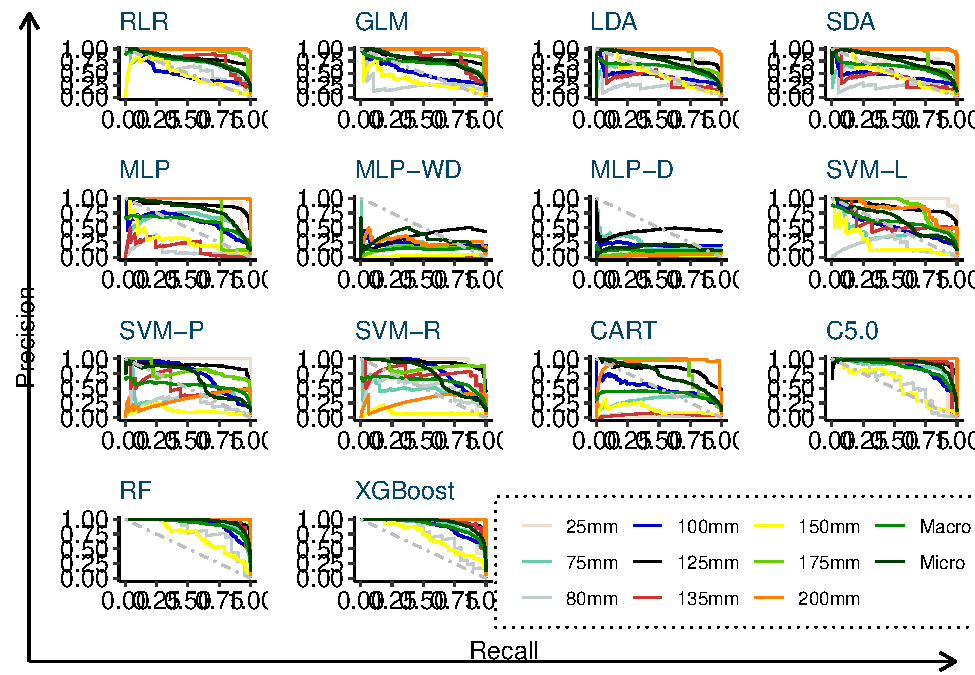
\includegraphics{sl-inf-cairs-2301_files/figure-latex/PRplots-1.pdf}

\begin{Shaded}
\begin{Highlighting}[]
\FunctionTok{ggsave}\NormalTok{(}\AttributeTok{filename =} \StringTok{"results/plt\_AUC\_PR.jpeg"}\NormalTok{,}\AttributeTok{plot =} \FunctionTok{last\_plot}\NormalTok{(),}
       \AttributeTok{device =} \StringTok{"jpeg"}\NormalTok{,}\AttributeTok{width =} \DecValTok{1109}\SpecialCharTok{/}\DecValTok{96}\NormalTok{,}\AttributeTok{height =} \DecValTok{1482}\SpecialCharTok{/}\DecValTok{96}\NormalTok{,}\AttributeTok{dpi =} \DecValTok{600}\NormalTok{)}
\end{Highlighting}
\end{Shaded}

\begin{quote}
\hypertarget{auc-scores}{%
\subsubsection{AUC scores}\label{auc-scores}}
\end{quote}

\begin{Shaded}
\begin{Highlighting}[]
\NormalTok{AUC\_data\_all}\OtherTok{\textless{}{-}}\FunctionTok{t}\NormalTok{(}
  \FunctionTok{data.frame}\NormalTok{(}\StringTok{"RLR\_ROC"}\OtherTok{=}\FunctionTok{unlist}\NormalTok{(AUC\_rlr}\SpecialCharTok{$}\NormalTok{ROC}\SpecialCharTok{$}\NormalTok{AUC}\SpecialCharTok{$}\NormalTok{fit\_01regLogistic),}
             \StringTok{"GLM\_ROC"}\OtherTok{=}\FunctionTok{unlist}\NormalTok{(AUC\_glm}\SpecialCharTok{$}\NormalTok{ROC}\SpecialCharTok{$}\NormalTok{AUC}\SpecialCharTok{$}\NormalTok{fit\_02glmnet),}
             \StringTok{"LDA\_ROC"}\OtherTok{=}\FunctionTok{unlist}\NormalTok{(AUC\_lda}\SpecialCharTok{$}\NormalTok{ROC}\SpecialCharTok{$}\NormalTok{AUC}\SpecialCharTok{$}\NormalTok{fit\_03lda),}
             \StringTok{"SDA\_ROC"}\OtherTok{=}\FunctionTok{unlist}\NormalTok{(AUC\_sda}\SpecialCharTok{$}\NormalTok{ROC}\SpecialCharTok{$}\NormalTok{AUC}\SpecialCharTok{$}\NormalTok{fit\_04sda),}
             \StringTok{"MLP\_ROC"}\OtherTok{=}\FunctionTok{unlist}\NormalTok{(AUC\_mlp}\SpecialCharTok{$}\NormalTok{ROC}\SpecialCharTok{$}\NormalTok{AUC}\SpecialCharTok{$}\NormalTok{fit\_05mlp),}
             \StringTok{"MLP{-}WD\_ROC"}\OtherTok{=}\FunctionTok{unlist}\NormalTok{(AUC\_mlpWD}\SpecialCharTok{$}\NormalTok{ROC}\SpecialCharTok{$}\NormalTok{AUC}\SpecialCharTok{$}\NormalTok{fit\_07mlpKerasDropout),}
             \StringTok{"MLP{-}D\_ROC"}\OtherTok{=}\FunctionTok{unlist}\NormalTok{(AUC\_mlpD}\SpecialCharTok{$}\NormalTok{ROC}\SpecialCharTok{$}\NormalTok{AUC}\SpecialCharTok{$}\NormalTok{fit\_06mlpWD),}
             \StringTok{"SVM{-}L\_ROC"}\OtherTok{=}\FunctionTok{unlist}\NormalTok{(AUC\_svml}\SpecialCharTok{$}\NormalTok{ROC}\SpecialCharTok{$}\NormalTok{AUC}\SpecialCharTok{$}\NormalTok{fit\_08svml),}
             \StringTok{"SVM{-}P\_ROC"}\OtherTok{=}\FunctionTok{unlist}\NormalTok{(AUC\_svmp}\SpecialCharTok{$}\NormalTok{ROC}\SpecialCharTok{$}\NormalTok{AUC}\SpecialCharTok{$}\NormalTok{fit\_09svmp),}
             \StringTok{"SVM{-}R\_ROC"}\OtherTok{=}\FunctionTok{unlist}\NormalTok{(AUC\_svmR}\SpecialCharTok{$}\NormalTok{ROC}\SpecialCharTok{$}\NormalTok{AUC}\SpecialCharTok{$}\NormalTok{fit\_10svmr),}
             \StringTok{"CART\_ROC"}\OtherTok{=}\FunctionTok{unlist}\NormalTok{(AUC\_CART}\SpecialCharTok{$}\NormalTok{ROC}\SpecialCharTok{$}\NormalTok{AUC}\SpecialCharTok{$}\NormalTok{fit\_11cart),}
             \StringTok{"C5\_ROC"}\OtherTok{=}\FunctionTok{unlist}\NormalTok{(AUC\_C5}\SpecialCharTok{$}\NormalTok{ROC}\SpecialCharTok{$}\NormalTok{AUC}\SpecialCharTok{$}\NormalTok{fit\_12C5),}
             \StringTok{"RF\_ROC"}\OtherTok{=}\FunctionTok{unlist}\NormalTok{(AUC\_RF}\SpecialCharTok{$}\NormalTok{ROC}\SpecialCharTok{$}\NormalTok{AUC}\SpecialCharTok{$}\NormalTok{fit\_13rf),}
             \StringTok{"XGB\_ROC"}\OtherTok{=}\FunctionTok{unlist}\NormalTok{(AUC\_xgb}\SpecialCharTok{$}\NormalTok{ROC}\SpecialCharTok{$}\NormalTok{AUC}\SpecialCharTok{$}\NormalTok{fit\_14xgb),}
             \StringTok{"RLR\_PR"}\OtherTok{=}\FunctionTok{unlist}\NormalTok{(AUC\_rlr}\SpecialCharTok{$}\NormalTok{PR}\SpecialCharTok{$}\NormalTok{AUC}\SpecialCharTok{$}\NormalTok{fit\_01regLogistic),}
             \StringTok{"GLM\_PR"}\OtherTok{=}\FunctionTok{unlist}\NormalTok{(AUC\_glm}\SpecialCharTok{$}\NormalTok{PR}\SpecialCharTok{$}\NormalTok{AUC}\SpecialCharTok{$}\NormalTok{fit\_02glmnet),}
             \StringTok{"LDA\_PR"}\OtherTok{=}\FunctionTok{unlist}\NormalTok{(AUC\_lda}\SpecialCharTok{$}\NormalTok{PR}\SpecialCharTok{$}\NormalTok{AUC}\SpecialCharTok{$}\NormalTok{fit\_03lda),}
             \StringTok{"SDA\_PR"}\OtherTok{=}\FunctionTok{unlist}\NormalTok{(AUC\_sda}\SpecialCharTok{$}\NormalTok{PR}\SpecialCharTok{$}\NormalTok{AUC}\SpecialCharTok{$}\NormalTok{fit\_04sda),}
             \StringTok{"MLP\_PR"}\OtherTok{=}\FunctionTok{unlist}\NormalTok{(AUC\_mlp}\SpecialCharTok{$}\NormalTok{PR}\SpecialCharTok{$}\NormalTok{AUC}\SpecialCharTok{$}\NormalTok{fit\_05mlp),}
             \StringTok{"MLP{-}WD\_PR"}\OtherTok{=}\FunctionTok{unlist}\NormalTok{(AUC\_mlpWD}\SpecialCharTok{$}\NormalTok{PR}\SpecialCharTok{$}\NormalTok{AUC}\SpecialCharTok{$}\NormalTok{fit\_07mlpKerasDropout),}
             \StringTok{"MLP{-}D\_PR"}\OtherTok{=}\FunctionTok{unlist}\NormalTok{(AUC\_mlpD}\SpecialCharTok{$}\NormalTok{PR}\SpecialCharTok{$}\NormalTok{AUC}\SpecialCharTok{$}\NormalTok{fit\_06mlpWD),}
             \StringTok{"SVM{-}L\_PR"}\OtherTok{=}\FunctionTok{unlist}\NormalTok{(AUC\_svml}\SpecialCharTok{$}\NormalTok{PR}\SpecialCharTok{$}\NormalTok{AUC}\SpecialCharTok{$}\NormalTok{fit\_08svml),}
             \StringTok{"SVM{-}P\_PR"}\OtherTok{=}\FunctionTok{unlist}\NormalTok{(AUC\_svmp}\SpecialCharTok{$}\NormalTok{PR}\SpecialCharTok{$}\NormalTok{AUC}\SpecialCharTok{$}\NormalTok{fit\_09svmp),}
             \StringTok{"SVM{-}R\_PR"}\OtherTok{=}\FunctionTok{unlist}\NormalTok{(AUC\_svmR}\SpecialCharTok{$}\NormalTok{PR}\SpecialCharTok{$}\NormalTok{AUC}\SpecialCharTok{$}\NormalTok{fit\_10svmr),}
             \StringTok{"CART\_PR"}\OtherTok{=}\FunctionTok{unlist}\NormalTok{(AUC\_CART}\SpecialCharTok{$}\NormalTok{PR}\SpecialCharTok{$}\NormalTok{AUC}\SpecialCharTok{$}\NormalTok{fit\_11cart),}
             \StringTok{"C5\_PR"}\OtherTok{=}\FunctionTok{unlist}\NormalTok{(AUC\_C5}\SpecialCharTok{$}\NormalTok{PR}\SpecialCharTok{$}\NormalTok{AUC}\SpecialCharTok{$}\NormalTok{fit\_12C5),}
             \StringTok{"RF\_PR"}\OtherTok{=}\FunctionTok{unlist}\NormalTok{(AUC\_RF}\SpecialCharTok{$}\NormalTok{PR}\SpecialCharTok{$}\NormalTok{AUC}\SpecialCharTok{$}\NormalTok{fit\_13rf),}
             \StringTok{"XGB\_PR"}\OtherTok{=}\FunctionTok{unlist}\NormalTok{(AUC\_xgb}\SpecialCharTok{$}\NormalTok{PR}\SpecialCharTok{$}\NormalTok{AUC}\SpecialCharTok{$}\NormalTok{fit\_14xgb)))}


\NormalTok{knitr}\SpecialCharTok{::}\FunctionTok{kable}\NormalTok{(AUC\_data\_all,}\AttributeTok{escape =}\NormalTok{ F,}\AttributeTok{digits =} \DecValTok{4}\NormalTok{,}\AttributeTok{format =} \StringTok{"simple"}\NormalTok{)}
\end{Highlighting}
\end{Shaded}

\begin{longtable}[]{@{}lrrrrrrrrrrr@{}}
\toprule()
& 25mm & 75mm & 80mm & 100mm & 125mm & 135mm & 150mm & 175mm & 200mm &
macro & micro \\
\midrule()
\endhead
RLR\_ROC & 0.9999 & 0.9178 & 0.9890 & 0.7621 & 0.8823 & 0.9932 & 0.9265
& 0.9957 & 1.0000 & 0.9406 & 0.9633 \\
GLM\_ROC & 1.0000 & 0.9231 & 0.9756 & 0.7841 & 0.8772 & 0.9951 & 0.9088
& 0.9938 & 0.9999 & 0.9397 & 0.9639 \\
LDA\_ROC & 0.9973 & 0.8956 & 0.9724 & 0.7819 & 0.8831 & 0.9746 & 0.9282
& 0.9819 & 0.9998 & 0.9349 & 0.9508 \\
SDA\_ROC & 0.9973 & 0.8951 & 0.9724 & 0.7819 & 0.8833 & 0.9746 & 0.9282
& 0.9780 & 0.9998 & 0.9345 & 0.9506 \\
MLP\_ROC & 0.9992 & 0.9141 & 0.8985 & 0.8375 & 0.9318 & 0.7281 & 0.8863
& 0.8829 & 1.0000 & 0.8975 & 0.9516 \\
MLP.WD\_ROC & 0.4709 & 0.5027 & 0.5292 & 0.4905 & 0.5368 & 0.4136 &
0.3404 & 0.5141 & 0.1860 & 0.4427 & 0.6726 \\
MLP.D\_ROC & 0.2475 & 0.4901 & 0.3895 & 0.4559 & 0.4150 & 0.3870 &
0.3780 & 0.7891 & 0.9146 & 0.4963 & 0.8169 \\
SVM.L\_ROC & 0.9999 & 0.7959 & 0.9452 & 0.7748 & 0.8993 & 0.9917 &
0.8069 & 0.9784 & 0.9874 & 0.9088 & 0.9087 \\
SVM.P\_ROC & 1.0000 & 0.7790 & 0.9640 & 0.8364 & 0.9340 & 0.9899 &
0.7986 & 0.9858 & 0.9494 & 0.9152 & 0.9065 \\
SVM.R\_ROC & 0.9899 & 0.8360 & 0.9882 & 0.8905 & 0.9562 & 0.9956 &
0.7574 & 0.9928 & 0.9428 & 0.9277 & 0.9218 \\
CART\_ROC & 0.7920 & 0.7915 & 0.8189 & 0.8005 & 0.8615 & 0.8405 & 0.8141
& 0.9648 & 0.9982 & 0.8536 & 0.9413 \\
C5\_ROC & 0.9823 & 0.9679 & 0.9179 & 0.9459 & 0.9727 & 0.9916 & 0.9339 &
1.0000 & 1.0000 & 0.9679 & 0.9859 \\
RF\_ROC & 1.0000 & 0.9833 & 0.9888 & 0.9704 & 0.9861 & 0.9993 & 0.9726 &
0.9999 & 1.0000 & 0.9888 & 0.9938 \\
XGB\_ROC & 0.9991 & 0.9759 & 0.9890 & 0.9625 & 0.9803 & 0.9991 & 0.9790
& 0.9996 & 1.0000 & 0.9871 & 0.9920 \\
RLR\_PR & 0.9898 & 0.7017 & 0.6274 & 0.4998 & 0.8224 & 0.8022 & 0.4595 &
0.9641 & 0.9992 & 0.7575 & 0.7717 \\
GLM\_PR & 1.0000 & 0.7126 & 0.2643 & 0.5068 & 0.8110 & 0.8517 & 0.3317 &
0.9536 & 0.9975 & 0.7078 & 0.7755 \\
LDA\_PR & 0.6947 & 0.5863 & 0.2621 & 0.4484 & 0.8412 & 0.3973 & 0.4902 &
0.8877 & 0.9969 & 0.6175 & 0.7508 \\
SDA\_PR & 0.7269 & 0.5856 & 0.2621 & 0.4483 & 0.8412 & 0.3979 & 0.4896 &
0.8868 & 0.9969 & 0.6209 & 0.7494 \\
MLP\_PR & 0.9571 & 0.6200 & 0.1120 & 0.5903 & 0.8881 & 0.1624 & 0.2919 &
0.7961 & 0.9997 & 0.5980 & 0.8043 \\
MLP.WD\_PR & 0.0086 & 0.2309 & 0.0157 & 0.2069 & 0.4359 & 0.0131 &
0.0277 & 0.0639 & 0.0304 & 0.1146 & 0.1683 \\
MLP.D\_PR & 0.0058 & 0.1892 & 0.0105 & 0.2112 & 0.3595 & 0.0126 & 0.0263
& 0.1449 & 0.2677 & 0.1361 & 0.3113 \\
SVM.L\_PR & 0.9908 & 0.4253 & 0.1825 & 0.5231 & 0.8550 & 0.5918 & 0.2227
& 0.8456 & 0.8142 & 0.6005 & 0.6274 \\
SVM.P\_PR & 1.0000 & 0.3551 & 0.2373 & 0.7353 & 0.8828 & 0.5376 & 0.1155
& 0.7911 & 0.3189 & 0.5464 & 0.6529 \\
SVM.R\_PR & 0.9126 & 0.4655 & 0.4979 & 0.7995 & 0.9391 & 0.7429 & 0.0842
& 0.8721 & 0.2986 & 0.6195 & 0.7210 \\
CART\_PR & 0.0221 & 0.3015 & 0.0418 & 0.4975 & 0.8207 & 0.0528 & 0.1378
& 0.8437 & 0.9331 & 0.4049 & 0.7250 \\
C5\_PR & 0.9311 & 0.8728 & 0.6082 & 0.8643 & 0.9543 & 0.9354 & 0.5606 &
1.0000 & 1.0000 & 0.8523 & 0.9280 \\
RF\_PR & 0.9951 & 0.9389 & 0.8003 & 0.9180 & 0.9809 & 0.9757 & 0.7175 &
0.9992 & 1.0000 & 0.9186 & 0.9633 \\
XGB\_PR & 0.9592 & 0.9076 & 0.7405 & 0.8865 & 0.9750 & 0.9623 & 0.7038 &
0.9965 & 1.0000 & 0.8985 & 0.9499 \\
\bottomrule()
\end{longtable}

\begin{Shaded}
\begin{Highlighting}[]
\FunctionTok{write.csv}\NormalTok{(AUC\_data\_all,}\StringTok{"results/AUC\_Data\_all.csv"}\NormalTok{)}
\end{Highlighting}
\end{Shaded}


\end{document}
